\chapter{Article I: A Ray-Tracing-Enhanced Lagrangian Particle Tracking Framework for Ice Accretion Applications}\label{sec:lagArticle}

%% Abstract
\textit
{
%% Text of abstract
This paper presents the development of a Lagrangian particle-tracking solver for ice accretion simulations on distributed-memory systems for aircraft applications. The solver is implemented within CHAMPS, an in-house multiphysics framework. The primary aim of this work is to enhance the robustness, accuracy, and computational efficiency of Lagrangian droplet tracking. To this end, a face-to-face tracking scheme is employed for robust boundary-intersection detection, combined with a ray-tracing–enhanced bilinear patch intersection technique to improve performance and scalability. An impact-neighbor identification strategy enables smooth water-catch distributions with a reduced number of droplets, while a hybrid Eulerian– Lagrangian adaptive seeding method automates droplet initialization. Supercooled large droplet (SLD) effects are incorporated to better align predictions with experimental data. A scalable parallel implementation is employed to enable efficient execution on distributed-memory architectures. Results demonstrate favorable verification against Eulerian formulations and improved accuracy relative to experimental data. Compared to existing Lagrangian tracking approaches, the proposed framework provides improved robustness in boundary-intersection detection, increased accuracy in collection efficiency predictions, and reduced computational cost, while maintaining scalability on distributed-memory systems.
}

\section{Introduction}
Particle-laden flows have long been a subject of scientific investigation due to their prevalence in numerous applications ranging from climate prediction \cite{climate} to combustion systems \cite{vaango2015cfd} and up to aeronautical applications \cite{rendall2014finite, bellosta2023lagrangian, BALDAN2023105856, sabri2024study}. A key challenge lies in the large number of particles required for high-fidelity simulations, which imposes significant computational demands. With recent advances in high-performance computing (HPC) on distributed systems, there is a growing need to optimize computational frameworks for tracking vast particle populations.

One application of interest for this study is ice accretion in aviation—a phenomenon that occurs when an aircraft traverses a supercooled moist cloud. Ice accretion can severely degrade aerodynamic performance \cite{lynch2001effects, cao2015aircraft}, making accurate prediction essential for flight safety \cite{CAO2018353}. The aviation industry increasingly relies on advanced numerical tools to forecast and mitigate the effect of ice formation, with water catch simulations playing a pivotal role in identifying droplet impingement locations. 

Recent Ice Prediction Workshops \cite{laurendeau2022summary, laurendeau2024summary} showcase that participants are leaning more toward using Eulerian droplet tracking methods \cite{ICEPAC, JAXA, FENSAP, ONERA, CIRA}. These methods adopt the same computational framework as the flow solver, hence presenting a great advantage in ease of implementation and computational efficiency. However, the Eulerian model still faces challenges in accurately representing complex droplet physics, such as splashing. Conversely, Lagrangian solvers, while more physically representative, have traditionally suffered from low computational efficiency. Nonetheless, modern HPC developments offer a promising pathway for reintroducing Lagrangian approaches in industrial ice accretion prediction tools.

Significant progress has been made in particle-laden flow simulations using the Lagrangian formulation, particularly for ice accretion, with recent studies highlighting strategies to overcome computational challenges. For instance, \cite{BALDAN2023105856} adapts the grid partitioning scheme based on particle trajectories, while \cite{sabri2024study} employs a dynamic load-balancing approach in which a dedicated computational rank redistributes droplets across the remaining ranks. However, further work is required to suppress oscillatory behavior \cite{Moula_2023} not seen in Eulerian results as well as to automate seeding-grid generation and develop computationally efficient techniques that improve accuracy without increasing computational cost. This work addresses several limitations of existing Lagrangian droplet tracking approaches. In particular, a face-to-face tracking strategy is implemented to improve the robustness and efficiency of boundary-intersection detection. To alleviate oscillations and spurious irregularities in the resulting surface-based numerical results, neighboring boundary cells are identified using the gradient stencil, enabling smoother surface results without requiring an excessive number of droplets. A ray-tracing–enhanced bilinear patch intersection technique is further employed to reduce intersection cost and improve solver scalability. In addition, a hybrid Eulerian–Lagrangian adaptive seeding strategy is introduced for large-scale configurations to automate droplet initialization and minimize user intervention. Supercooled large droplet (SLD) physics are incorporated in both the standalone Lagrangian and hybrid Eulerian–Lagrangian solvers to achieve predictions that align more closely with experimental observations. Finally, a hybrid MPI–OpenMP-like parallelization strategy based on Chapel paradigms is employed to enhance computational efficiency on distributed-memory systems. The paper is structured as follows: Section~\ref{sec:subsec1} reviews droplet tracking techniques in ice accretion applications and introduces the proposed Lagrangian approach. Section~\ref{sec:solverEnhacements} details the solver enhancements, including ray-tracing–driven face traversal, adaptive seeding, computation of collection efficiency with a gradient-stencil weighting strategy, incorporation of supercooled large droplet (SLD) effects, and the parallelization strategy for improved performance. Section~\ref{sec:Results} presents and analyzes benchmark test cases, highlighting key observations and trends. Finally, Section~\ref{sec:Conclusion} summarizes the main findings and outlines future research directions.

% %% Use \subsection commands to start a subsection.
\section{Droplet Tracking Techniques}
\label{sec:subsec1}

\subsection{Droplet Tracking Approaches for Ice Accretion}

Water droplet tracking is a key component of ice accretion simulations, as it determines both impingement locations and the amount of water collected on solid surfaces. Numerous approaches have been proposed in the literature, all aiming to balance robustness, accuracy, and computational efficiency.

Historically, early ice accretion solvers such as LEWICE \cite{wright1995users} relied on Lagrangian tracking, in which individual droplet trajectories are computed by solving their equations of motion. While well suited to panel-based potential-flow solvers, the extension of this approach to modern RANS-based frameworks introduces additional complexity due to the need for repeated interpolation of flow quantities at droplet locations.

To address these limitations, Eulerian approaches \cite{bourgault1999finite} were introduced, modeling droplets as a continuous dispersed phase governed by transport equations for momentum and volume fraction $\alpha$ (Fig.~\ref{fig:EulerianSolverResults}). This formulation integrates naturally within flow solvers and offers excellent computational efficiency and scalability . However, accurately representing complex droplet physics, such as splashing and secondary breakup, remains challenging and often computationally expensive.

\begin{figure}[htbp] 
    \centering
    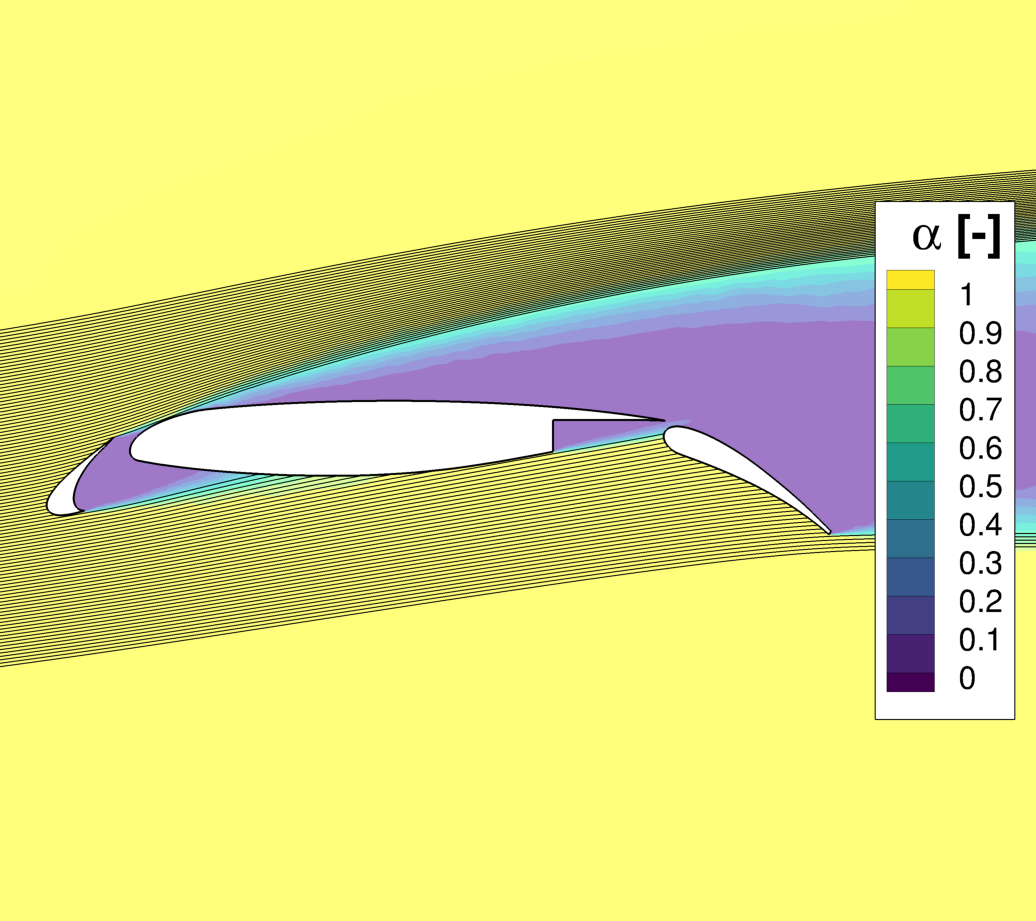
\includegraphics[trim={0cm 6cm 0cm 4cm},clip,width=0.5\textwidth]{FIGURES/LAGRANGIAN_ARTICLE/DropletVolumeFraction.png}
    \caption{Example of Eulerian solver results : Countour of water volume fraction $\alpha$ with droplet trajectories streamlines.}
    \label{fig:EulerianSolverResults}
\end{figure}
 
Recent studies have nonetheless highlighted the advantages of Lagrangian tracking for capturing localized phenomena, particularly in the formation of scalloped ice structures \cite{ozcer2024numerical}. By resolving individual droplet trajectories, the Lagrangian approach can better capture localized enrichment effects and fine-scale surface features that may be smoothed out in Eulerian formulations (e.g. between scallops or small-scale ice features).


\subsection{Lagrangian Droplet Tracking}
Lagrangian droplet tracking is based on integrating the equation of motion from Newton’s second law (Eq. \ref{eq:eqOfMotion}) for each droplet individually. First, the velocity of the droplet $\boldsymbol{u_d}$ is calculated using the air flow velocity $\boldsymbol{u_a}$ and the buoyancy-corrected gravitational acceleration $(\rho_d - \rho_a)/\rho_d\,\boldsymbol{g}$. Then a second integration (Eq. \ref{eq:eqOfPos}) gives the position of the droplet $\boldsymbol{x_d}$. For the present work, the forces considered are the drag force as a result of the fluid flow and the gravitational force acting on the droplet. The scalar function for the drag force $\textbf{F}$ can be found using the droplet local Reynolds number based on the relative velocity $\| \boldsymbol{u_a} -  \boldsymbol{u_d}\|$ and droplet diameter $D$. This leads to a force coefficient \textit{F} (Eq. \ref{eq:forceCoef}) using $C_D$, the drag coefficient of the droplet, $\rho_a$, the air density and $\rho_w$, the water density:


\begin{equation}
\frac{d\boldsymbol{u_d}}{dt} = \frac{\textbf{f}}{m} + \textbf{g} = F( \boldsymbol{u_a}- \boldsymbol{u_d}) + \frac{\rho_d-\rho_a}{\rho_d}\textbf{g}
\label{eq:eqOfMotion}
\end{equation}

\begin{equation}
\frac{d\boldsymbol{x_d}}{dt} = \boldsymbol{u_d}
\label{eq:eqOfPos}
\end{equation}

\begin{equation}
F  = \frac{3 C_D  \rho_a \| \boldsymbol{u_a} -  \boldsymbol{u_d}\| }{4 \rho_w D}
\label{eq:forceCoef}
\end{equation}

\noindent The key hypotheses to ensure the validity of this model are the following:

\begin{itemize}
        \item The mass of the droplet is supposed constant and does not change over time before colliding with the geometry;
        \item The droplets are independent from one another, therefore collisions and coalescence are not considered;
        \item The droplet concentration do not affect the fluid flow;
        \item The effects of the turbulence are neglected on the droplets;
        \item The droplets do not rotate or have lift.
        \item The phase change within the droplets is not considered, as the solver is limited to computing the deposited liquid water mass under the quasi-steady icing hypothesis\cite{KIND1998257}.
\end{itemize}

One of the main problems of Lagrangian droplets trackers in such applications is that droplet trajectories rarely coincide with the flow grid. The integration of Eq. \ref{eq:eqOfMotion} relies on interpolation of the flow velocity depending on the droplet position. Therefore, after each integration, a relocating step is needed in order to pinpoint the exact location of the droplet inside the flow grid. The choice of the technique is based on accuracy, efficiency and stability. In the literature, various techniques have been developed for particle tracking. Tree-based search techniques \cite{press2007numerical} and more advanced auxiliary-grid approaches \cite{li2019fast}, illustrated in Fig.~\ref{fig:auxiliaryGrid}, provide a straightforward way to identify host cells for tracked droplets. However, both approaches incur significant computational and memory overheads and are difficult to deploy efficiently on distributed-memory systems.

\begin{figure}[htbp] 
    \centering
    \subfloat[Auxiliary grid tracking \cite{li2019fast}.]{%
        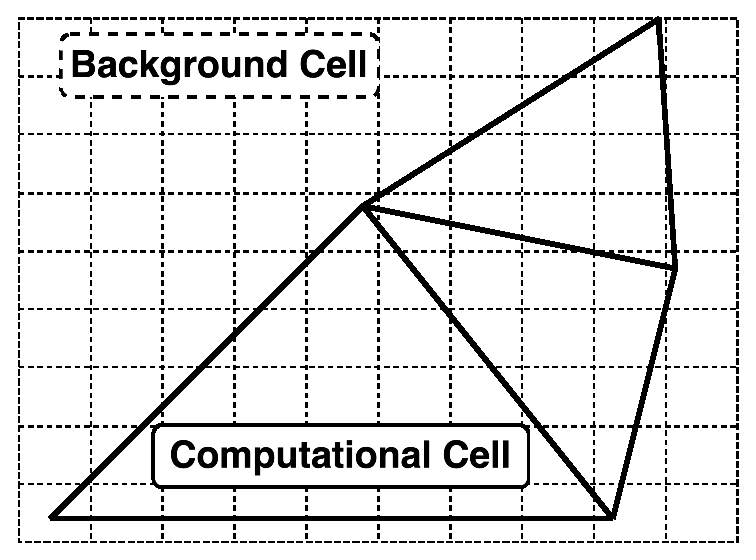
\includegraphics[width=0.32\textwidth]{FIGURES/LAGRANGIAN_ARTICLE/TrackingBackgroundGrid.eps}%
        \label{fig:auxiliaryGrid}%
        }%
        \hspace{0.1cm}
    \subfloat[\centering face-to-face tracking \cite{bellosta2023lagrangian} \newline (In Cell Positions).]{%
        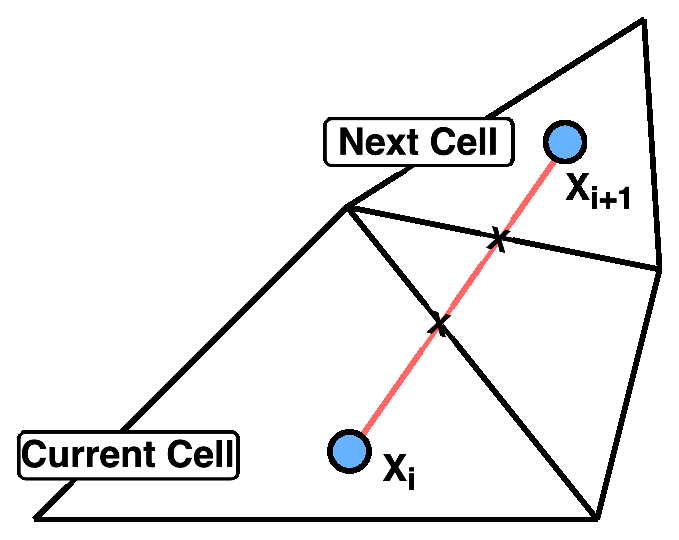
\includegraphics[width=0.32\textwidth]{FIGURES/LAGRANGIAN_ARTICLE/TrackingThroughCells.eps}%
        \label{fig:cell2cell}%
        }%
        \hspace{-0.1cm}
    \subfloat[ \centering face-to-face tracking \cite{rendall2014finite} \newline (On Face Positions).]{%
        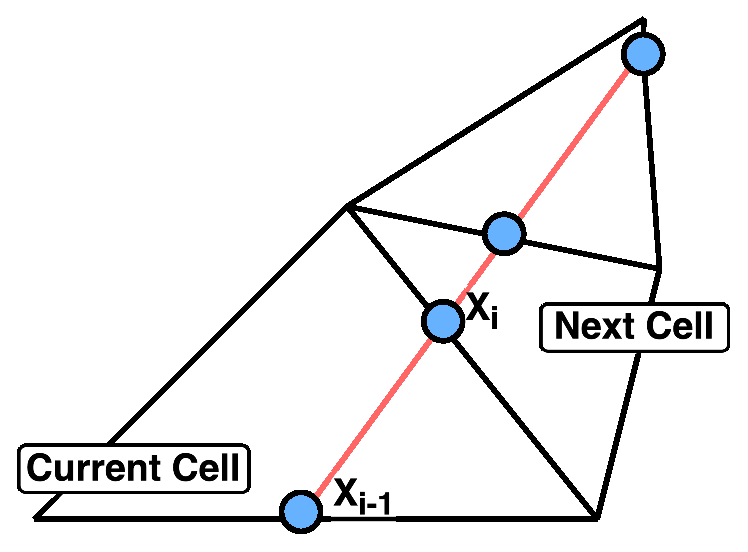
\includegraphics[width=0.32\textwidth]{FIGURES/LAGRANGIAN_ARTICLE/Trackingface2face.eps}
        \label{fig:face2face}%
        }%
    \caption{ Droplet tracking techniques.}
    \label{fig:lagrangianTracking}
\end{figure}


Face-to-face searching techniques \cite{bellosta2023lagrangian}, illustrated in Fig.~\ref{fig:cell2cell}, exploit the droplet’s previous position and velocity to locate its host cell by traversing mesh connectivity. These methods can become challenging to handle when droplets traverse near-wall zones, particularly in regions with strong gradients, where careful treatment and appropriate time-step selection are required to ensure robust impact detection.

The face-to-face tracking method presented by \cite{rendall2014finite} further refines this process using edge-to-cell (in 2D) or face-to-cell (in 3D) connectivity, as illustrated in Fig. \ref{fig:face2face}. Similarly to the previous method, a ray is casted based on the droplet velocity. Then the algorithm iteratively computes the nearest face intersection to find the next flow cell. This approach offers significant flexibility since the timestep becomes an adaptive by-product of the simulation. Specifically, a local timestep is calculated based on the droplet's residence time within each cell. This adaptability is important in Reynolds-Averaged Navier–Stokes (RANS) simulations, where fine meshes are needed to resolve near-wall flows and the resulting small cells demand reduced timesteps for accuracy and stability. An additional advantage of this method is its simplicity of implementation, as it leverages the same finite-volume framework used by the flow solver. Accordingly, the Lagrangian droplet tracking is performed on the same computational domain and unstructured mesh as the flow simulations. Moreover, the host cell is implicitly determined through mesh connectivity, eliminating the need for explicit host cell searches. The inherent alignment with the finite-volume solver ensures compatibility and seamless integration. These advantages collectively make it the preferred choice for particle tracking in this work.

The integration of Eq. \ref{eq:eqOfMotion} is achieved using a second order backward difference scheme \cite{rendall2014finite}:


\begin{equation}
a \boldsymbol{u_d}^n + b \boldsymbol{u_d}^{n-1} + c \boldsymbol{u_d}^{n-2} = F (\boldsymbol{u_a}-\boldsymbol{u_d}) + \textbf{g}
\label{eq:BDF1}
\end{equation}


\begin{equation}
 \boldsymbol{u_d}^{n} = \frac{F \boldsymbol{u_a} - b \boldsymbol{u_d}^{n-1}  - c \boldsymbol{u_d}^{n-2} +\textbf{g}}{a + F}
\label{eq:BDF2_Time}
\end{equation}

\begin{equation}
a = \frac{2\Delta t_c+\Delta t_{c-1}}{(\Delta t_c+\Delta t_{c-1})\Delta t_c}
\label{eq:alpha}
\end{equation}

\begin{equation}
b = \frac{-(\Delta t_c+\Delta t_{c-1})}{\Delta t_c\Delta t_{c-1}}
\label{eq:beta}
\end{equation}

\begin{equation}
c = \frac{\Delta t_c}{(\Delta t_c+\Delta t_{c-1})\Delta t_{c-1}}
\label{eq:gamma}
\end{equation}

\noindent where $\Delta t$ is the time step at the current iteration. The superscripts $n$, $n-1$, and $n-2$ represent time integration levels, while the subscripts $c$ and $c+1$ denote cell values. The algorithm presented in \cite{rendall2014finite} consists of an iterative process that ends up converging towards the droplet velocity. The flow velocity at the face $\boldsymbol{u_a}^n$ is calculated through averaging flow velocity across current and the next cell: 

\begin{equation}
    \boldsymbol{u_a}^n = \frac{1}{2} (\boldsymbol{u_a}_c + \boldsymbol{u_a}_{c+1})
\end{equation}

\noindent This presumes that the next cell is known in advance, hence the iterative process. At first, $\boldsymbol{u_d}^n$ is supposed to be equal to $\boldsymbol{u_d}^{n-1}$. Then, the nearest face intersection is computed on the basis of that assumption. This leads to calculating the time step along with the other local variables using Eqs. \ref{eq:alpha}, \ref{eq:beta}, and \ref{eq:gamma}. Finally, Eq. \ref{eq:BDF2_Time} is then used to calculate $\boldsymbol{u_d}^n$ and the process is iterated until there is a slight user specified difference between two consecutive iterations. It should be noted that the closest face intersection is made based on the mid-cell velocity :

\begin{equation}
    \boldsymbol{u_d}^{n-\frac{1}{2}} = \frac{1}{2} (\boldsymbol{u_d}^n + \boldsymbol{u_d}^{n-1})
\end{equation}

\noindent Due to high gradients near the wall, this method can reduce to the first order \cite{rendall2014finite}. To alleviate this problem, the flow gradient is used to interpolate the flow velocity from the center of the cell to the droplet position using the distance $\boldsymbol{d}$ between the two: 

\begin{equation}
\boldsymbol{u_a}_{face} = \boldsymbol{u_a}_{cell} + \nabla \cdot \boldsymbol{d}
\label{eq:faceFlow}
\end{equation}

\section{Improvements in Lagrangian Particle Tracking}
\label{sec:solverEnhacements}
\subsection{Ray--Quadrilateral Intersections in CFD Applications}
\label{subsec:ray_quad_cfd}

In computational fluid dynamics (CFD), determining the intersection between particle velocity rays and mesh elements is a critical step in computing particle trajectories. 
When meshes are composed of quadrilateral elements, intersection detection becomes notably more challenging. 
Quadrilateral faces are not guaranteed to be perfectly planar due to numerical discretization errors. 
This lack of coplanarity complicates the definition of a unique intersection plane, making classical planar ray--plane tests unreliable.

\begin{figure}[htb] 
\centering
    \subfloat[Step 0: Definition of the ray and bilinear patch geometry.]{%
        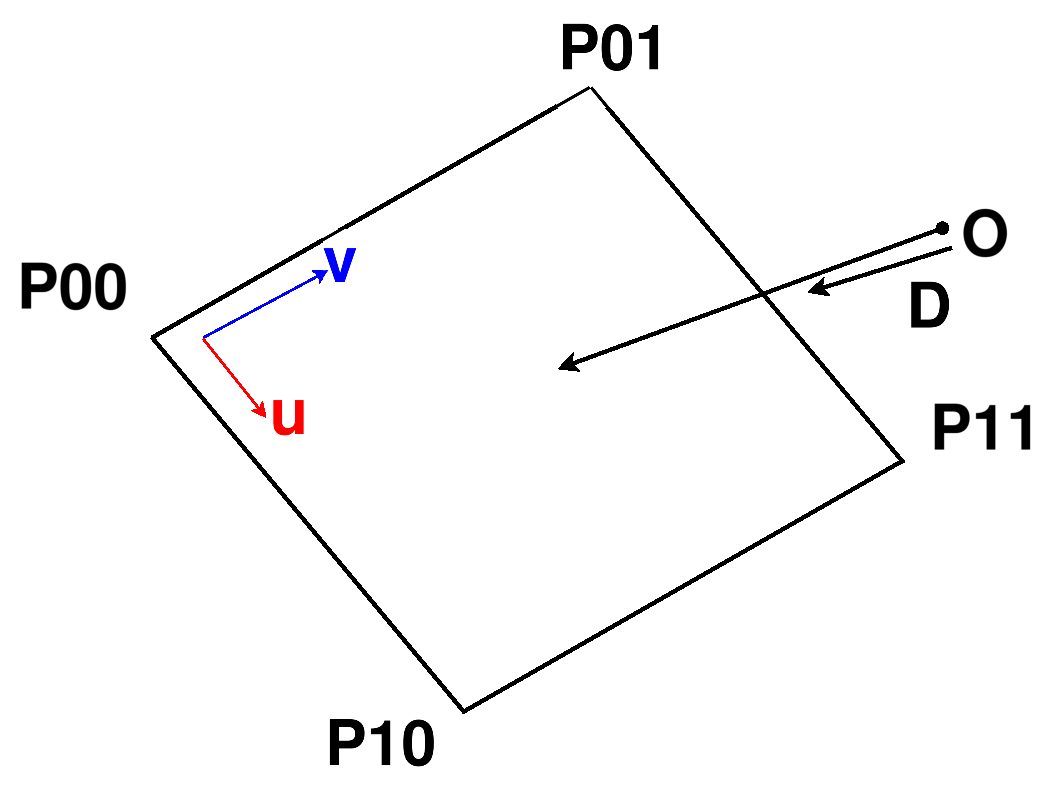
\includegraphics[width=0.3\textwidth]{FIGURES/LAGRANGIAN_ARTICLE/GARP_STEP_0.eps}%
        \label{fig:GARP_STEP0}%
        }%
    \hspace{0.1cm}
    \subfloat[Step 1: Determination of the intersection $u$-parameter along the bilinear patch.]{%
        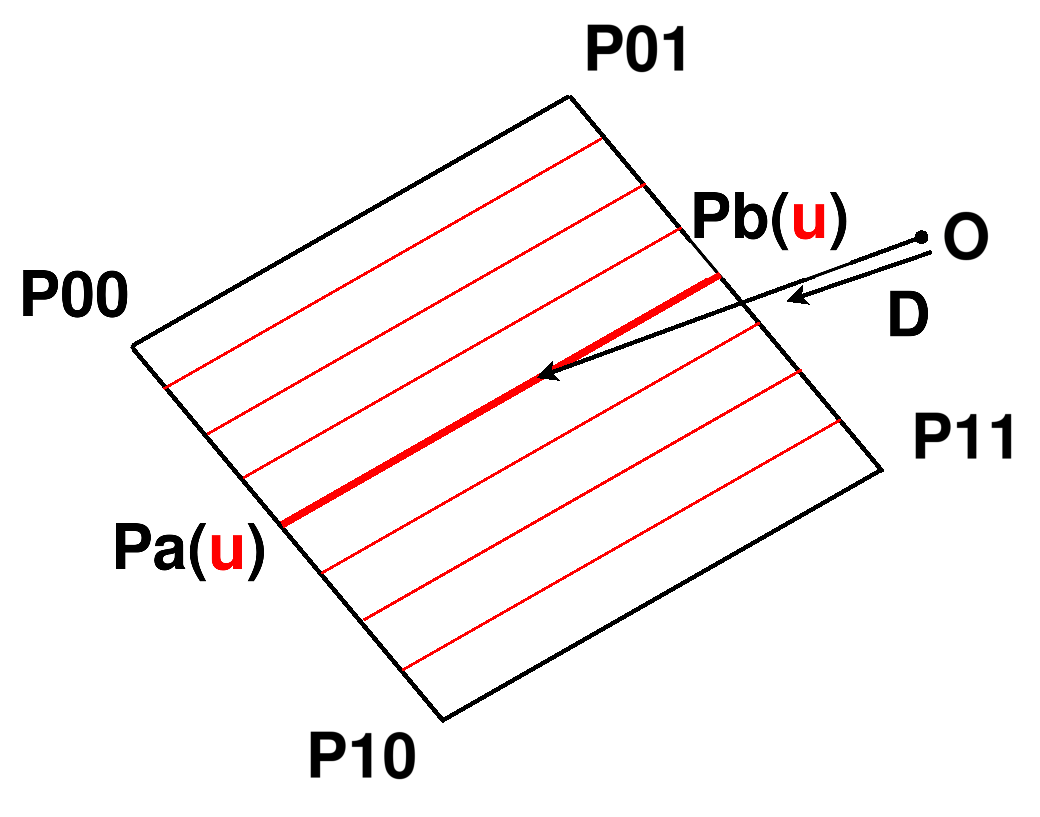
\includegraphics[width=0.3\textwidth]{FIGURES/LAGRANGIAN_ARTICLE/GARP_STEP_1.eps}%
        \label{fig:GARP_STEP1}%
        }%
    \hspace{0.1cm}
    \subfloat[Step 2: Determination of the intersection $v$-parameter along the bilinear patch.]{%
        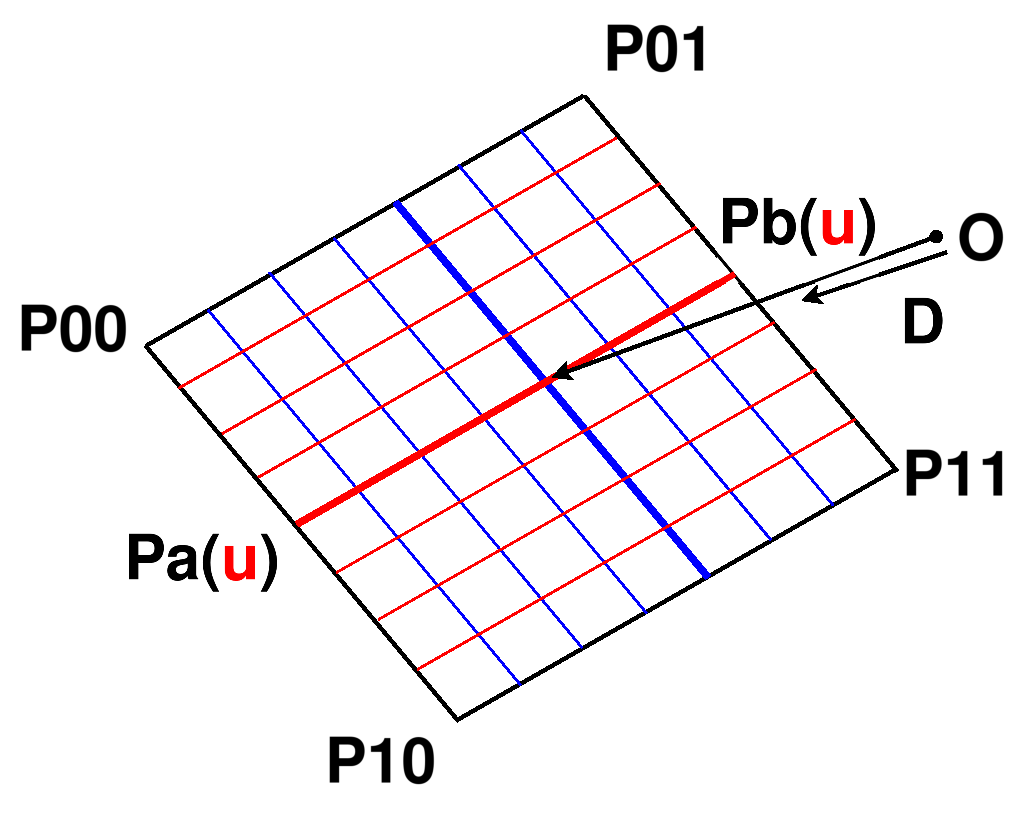
\includegraphics[width=0.3\textwidth]{FIGURES/LAGRANGIAN_ARTICLE/GARP_STEP_2.eps}%
        \label{fig:GARP_STEP2}%
        }%
        \caption{Steps for Ray--Bilinear Patch Intersection.}
\end{figure}

A commonly used workaround is to split each quadrilateral into two planar triangles and perform independent ray–triangle intersection tests, each solved following the method of \cite{M_ller_1997}. Although straightforward, this approach introduces artificial discontinuities along the internal diagonal, potentially causing small numerical inconsistencies and reduced computational efficiency. 
 A more consistent alternative is to represent each quadrilateral as a bilinear patch, parameterized in local coordinates $(u,v) \in [0,1]^2$, as illustrated in Fig.\ref{fig:GARP_STEP0}.
In this parametric representation, the surface is defined by bilinear interpolation of the four corner vertices, providing a continuous geometric mapping over the quadrilateral. This formulation allows intersections to be computed directly on the bilinear surface, maintaining geometric continuity across the element patch.

Recent advances in computer graphics have introduced highly optimized algorithms for ray--patch intersection. 
Among these, the GARP (Geometric Approach to Ray--Patch Intersections) method \cite{Reshetov_2019} offers a robust and efficient alternative to the algebraic formulation presented in \cite{Ramsey_2004}. It is this latter formulation that remains widely used in Lagrangian particle-tracking frameworks \cite{Haselbacher_2007, Kopper_2023}.

Ray–patch intersection aims to determine where a ray $\boldsymbol{r(t)}$ (Eq.\ref{eq:ray_param}), emitted from a given position, intersects a patch $\boldsymbol{p(u,v)}$ represented in parametric coordinates (Eq.\ref{eq:bilinear_patch}):

\begin{equation}
\boldsymbol{r}(t) = \boldsymbol{O} + t\boldsymbol{D}, \quad t \ge 0,
\label{eq:ray_param}
\end{equation}

\begin{equation}
\boldsymbol{p}(u,v) = (1-u)(1-v)\boldsymbol{p}_{00} + (1-u)v\boldsymbol{p}_{01}
+ u(1-v)\boldsymbol{p}_{10} + uv\boldsymbol{p}_{11}.
\label{eq:bilinear_patch}
\end{equation}

\noindent where $\boldsymbol{O}$ and $\boldsymbol{D}$ denote the ray origin and direction, respectively, and $\boldsymbol{p}_{ij}$ are the patch vertices. 
Equating Eqs.~\ref{eq:ray_param} and \ref{eq:bilinear_patch} yields a system of three equations that can be solved analytically \cite{Ramsey_2004}.  While this approach is conceptually simple and easy to implement, it introduces algebraic branching and conditional checks that can hinder computational performance. Instead of explicitly computing an intersection plane or solving high-order polynomial systems, the GARP method interprets the bilinear patch as a ruled surface obtained by linear interpolation between two opposite edges. The intersection procedure is carried out in two parametric stages, as illustrated in Fig.~\ref{fig:GARP_STEP1}--\ref{fig:GARP_STEP2}.

First, the intersection is searched along the $u$-parametric direction. For a given ray, the parameter $u$ is determined by enforcing coplanarity between the ray and the interpolated patch edge. This condition is expressed by setting the scalar triple product of the vectors $\boldsymbol{O}\boldsymbol{P}_a$, $\boldsymbol{P}_a\boldsymbol{P}_b$, and $\boldsymbol{D}$ to zero, which leads to a quadratic equation in $u$. Only solutions satisfying $u \in [0,1]$ are retained.

Once $u$ is determined, the corresponding interpolated segment $\boldsymbol{P}_a\boldsymbol{P}_b$ is fully defined. The second stage consists of determining the $v$-parametric coordinate by projecting the ray onto this segment and identifying the point that minimizes the distance between the ray and the segment. A valid intersection is obtained when $v \in [0,1]$, after which the ray parameter $t$ is computed. In the presence of multiple valid solutions, the intersection corresponding to the smallest positive value of $t$ is selected. The reader is referred to \cite{Reshetov_2019} for a detailed derivation of the algorithm, along with a discussion of numerical robustness and performance considerations.

To evaluate computational performance, one million random rays and quadrilateral patches were generated for intersection testing using both formulations, along with the traditional two-triangle method. 
Results demonstrate that both ray--patch methods outperform the two-triangle approach, with the GARP method achieving an additional $15\%$ speed-up over the analytic formulation of \cite{Ramsey_2004}. 
The implications of these improvements on the overall solver scalability are discussed in Section~\ref{sec:Results}.

\begin{table}[htb!]
\centering
\caption{Performance comparison of ray--quadrilateral intersection methods.}
\hspace*{-0.5cm}
\label{tab:quad_intersections}
\begin{tabular}{lcc}
\hline
\hline
\textbf{Intersection Method} & \textbf{Speed-up vs. Two-Triangles} & \textbf{Speed-up vs. \cite{Ramsey_2004}} \\
\hline\hline
Ramsey et al.~\cite{Ramsey_2004} & $51.3\%$ & 0 \% \\
GARP~\cite{Reshetov_2019} & $58.2\%$ & $14.2\%$ \\
\hline
\hline
\end{tabular}
\end{table}

\subsection{Adaptive Seeding}

In the Lagrangian droplet tracking framework, the strategic placement of the seeding grid plays a key role throughout the process. Typical seeding techniques \cite{wright2021automated} involve projecting the surface of interest onto a user-specified seeding plane and refining the grid to achieve optimal results. For instance, the process often begins with a simple rectangular grid, followed by launching a set of droplet trajectories. During tracking, the minimal wall distance is stored, a value typically accessible in RANS simulations. Cells whose minimum wall distance falls below a user-specified threshold, e.g., based on a reference length, are selectively refined to increase resolution in near-wall regions. While this approach is practical and straightforward to implement, careful consideration must be given to the projection of the surface. This is because the projection depends not only on the flow velocity direction but also on droplet diameter, which must account for gravitational effects. As a result, the placement of the seeding grid requires significant user expertise, especially when dealing with a wide range of flow conditions and droplet sizes.

To address these challenges and further automate the process, this work builds on the two-dimensional hybrid method proposed by \cite{papillon2022stochastic}, with the seeding technique is extended to three-dimensional simulations and parallelized. The approach traces droplet trajectories backward, starting from the surface of the geometry and extending upstream to a user-defined seeding plane. However, initiating this process within a Lagrangian solver poses challenges because the wall boundary condition in RANS simulations imposes zero velocity at the surface. To address this, the droplet velocity field obtained from an Eulerian solver (previously implemented in CHAMPS \cite{bourgault2019ice}) offers a practical solution, as droplets possess velocity before impacting the surface. The suggested method employs a hybrid Eulerian-Lagrangian seeding technique (illustrated in Fig. \ref{fig:hybridSeeding}), where an Eulerian solution is used to prepare the seeding grid for the Lagrangian solver.

\begin{figure}[htb] 
\centering
    \subfloat[Hybrid seeding \cite{papillon2022stochastic}.]{%
        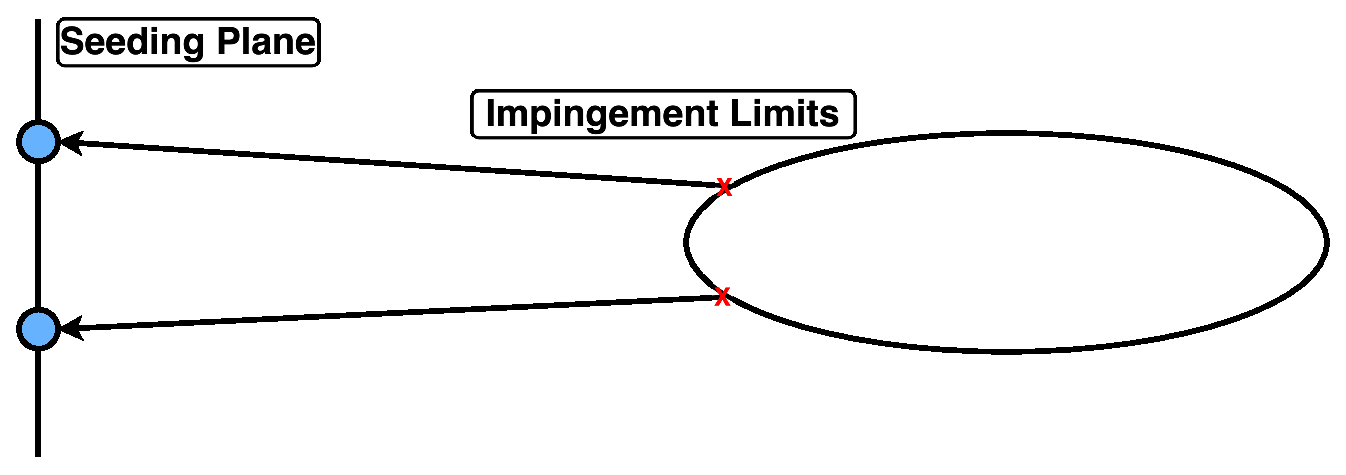
\includegraphics[trim={0cm 0cm 7cm 0cm},clip,width=0.6\textwidth]{FIGURES/LAGRANGIAN_ARTICLE/seedingPlane.eps}%
        \label{fig:hybridSeeding}%
        }%
        \hspace{0.1cm}
    \subfloat[Refinement technique.]{%
        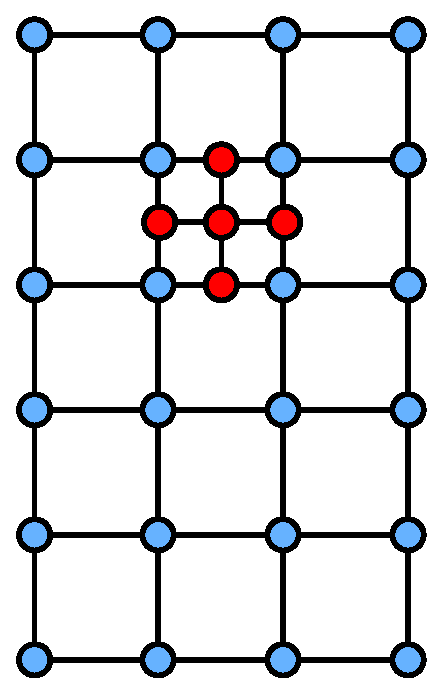
\includegraphics[width=0.245\textwidth]{FIGURES/LAGRANGIAN_ARTICLE/AdaptiveSeeding.eps}%
        \label{fig:seedingRef}%
        }%
        \caption{Adaptive seeding.}
\end{figure}

For the present work, the hybrid Eulerian-Lagrangian seeding technique is adopted. The Eulerian velocity field is used to perform reverse trajectory computations. Face intersections are computed based on the inverse droplet velocity, which is derived from the Eulerian solution. While Eulerian results are generally sufficient, Lagrangian results provide a more accurate representation of droplet physics, as will be demonstrated in Section ~\ref{sec:Results}. The process continues until the trajectory intersects a user-specified upstream seeding plane. To account for potential dissipation-induced errors, a safety margin can be incorporated into the computed seeding grid position. This automated approach significantly simplifies the process, reducing user input to specifying only the x-coordinate for the starting position. Once the limits are defined, a structured 2D rectangular grid (or 1D line grid for 2D problems) is generated, with nodes corresponding to the seeding positions.

 Another concern inherent in the Lagrangian method is determining the number of droplets used for accurate and smooth solutions. This work integrates an adaptive seeding technique as presented in \cite{bellosta2023lagrangian}. Initially, a simulation is conducted with a user-specified number of droplets, and subsequently, the seeding mesh is refined. For instance, if a droplet impacts the geometry, the corresponding seeding cell is then refined. The stop criterion for refinement is based on achieving a small residual for a global deposition metric (for instance, $\epsilon \approx 10^{-5}$). This metric is defined as the surface integral of the corresponding local quantity (Section~\ref{sec:collectionEfficiency}) over the body, providing a global measure of droplet deposition. After each refinement loop, the older droplets are restarted with the previous solution, hence only newly created droplets are simulated. The enhanced accuracy and smoothness  will be discussed in Section \ref{sec:Results}. 
 
 While adaptive seeding is an effective technique to achieve mesh convergence with the seeding grid, it requires a substantial number of initial droplets to accurately target complex geometries. In other words, there must be enough droplets impacting the geometry in the first refinement iteration in order to capture the geometry accurately. This can be challenging for large-scale geometries such as case 2.1 from the fifth edition of the High Lift Prediction Workshop (HLPW5) \cite{clark2025high} depicted in Fig. \ref{fig:crm}. The current technique employs structured rectangular meshes based on the bounding box (highlighted in red Fig. \ref{fig:seedingrid}), whose limits are obtained through backtracked droplets. However, this approach is not ideal for cases with multiple components. The overall bounding box becomes far too large and includes areas where unnecessary droplet trajectories are simulated. To circumvent this issue, a seeding grid per component is employed, as shown in Fig. \ref{fig:seedingrid}. Each component is simulated and refined individually before adding its contribution to the total results. This approach allows for better targeting each component without substantially increasing the number of droplets to be simulated.

\begin{figure}[ht]
\centering
    \subfloat[Case 2.1 - HLPW5 geometry.]{%
        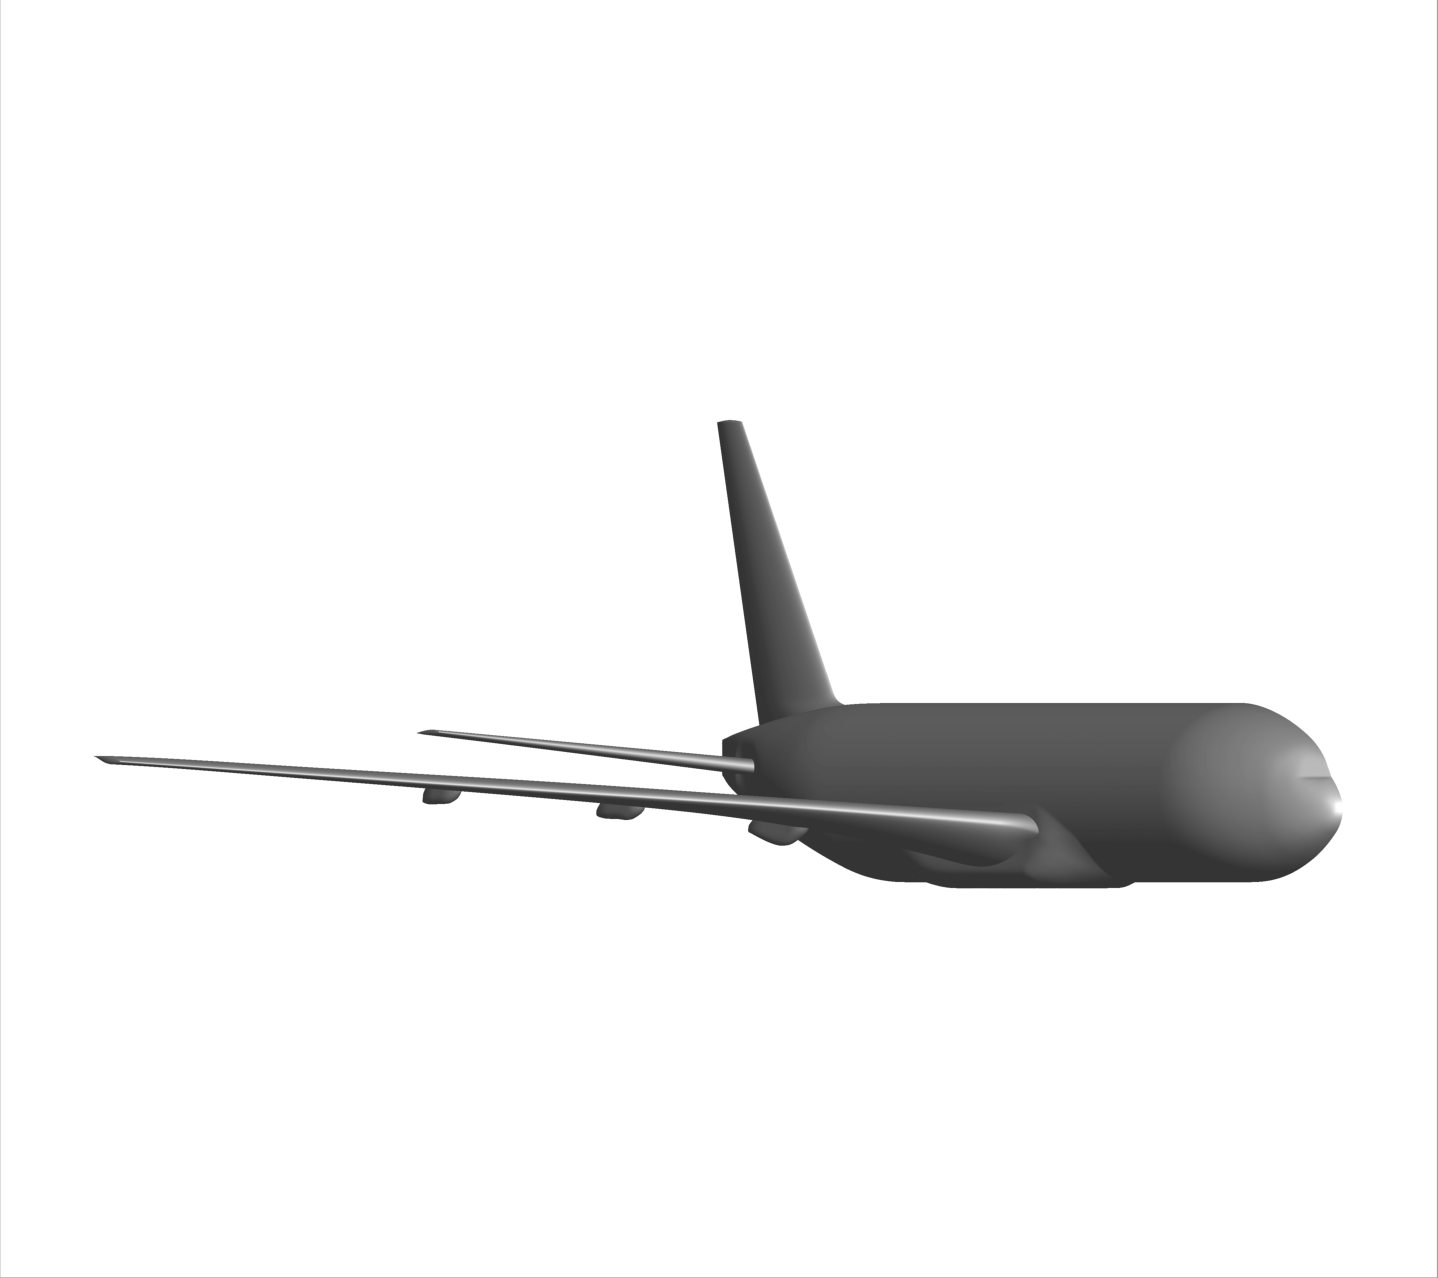
\includegraphics[trim={1cm 10cm 1cm 10cm},clip,width=0.48\textwidth]{FIGURES/LAGRANGIAN_ARTICLE/CRM.png}
        \label{fig:crm}%
        }%
    \subfloat[Large scale geometry seeding grid example.]{%
        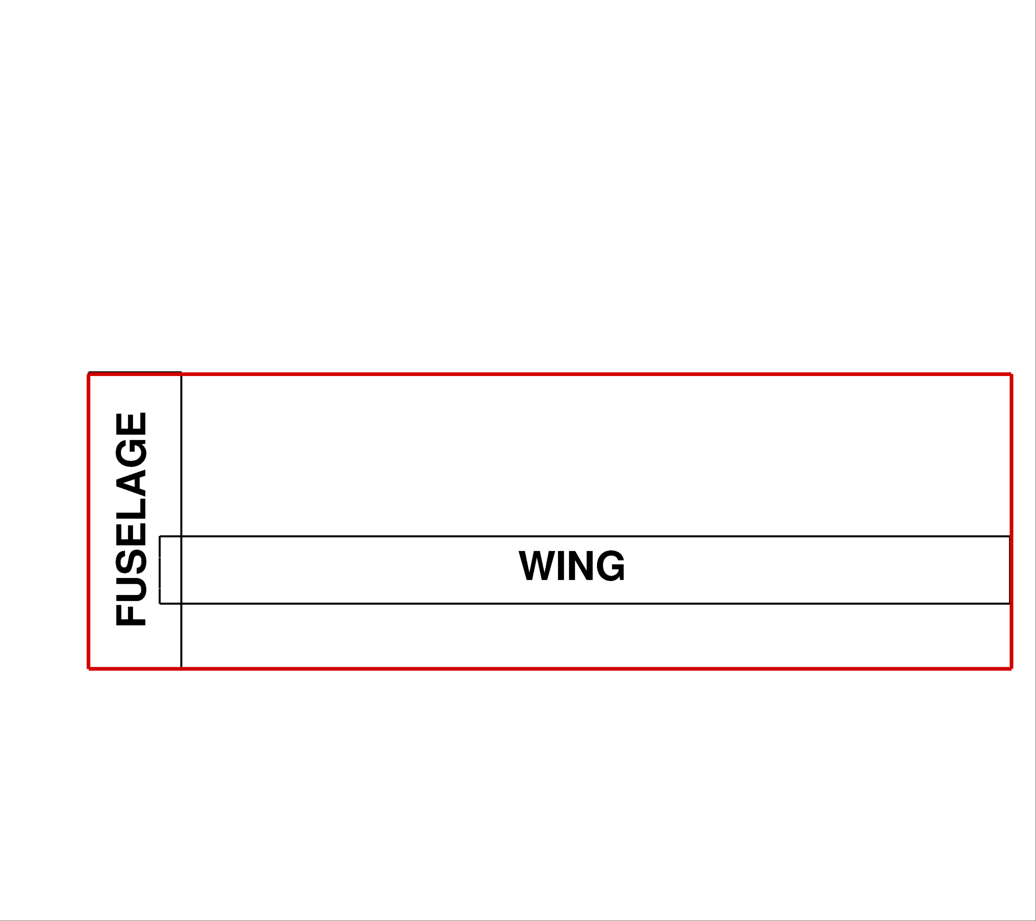
\includegraphics[trim={2cm 8cm 0.5cm 8cm},clip,width=0.48\textwidth]{FIGURES/LAGRANGIAN_ARTICLE/GRIDS.png}
        \label{fig:seedingrid}%
        }%
    \caption{Seeding technique for large scale geometries.}
    \label{fig:dropSeeding}
\end{figure}


\subsection{Collection Efficiency Computations}
\label{sec:collectionEfficiency}
In addition to impingement locations, water droplet tracking outputs the collection efficiency on the geometry. The latter measures how much of the upstream water is eventually captured by the geometry. This metric is essential for the thermodynamic exchanges in the ice accretion process, as it determines the incoming water mass flux on the surface. In the Lagrangian model, the traditional approach constructs a flow tube using three (triangle) or four (quadrilateral) trajectories in 3D, or two (line) trajectories in 2D, and tracks it downstream until it intersects the geometry. The collection efficiency $\beta$ is then computed as the ratio between the upstream area of the flow tube and the curvilinear area on the surface \cite{ruff1990users}:

\begin{equation}
    \beta = \frac{Upstream \, Area}{Impingement \, Area} = \frac{dy}{ds}
    \label{eq:betaEq}
\end{equation}

\noindent However, this method encounters several difficulties:
\begin{itemize}
    \item Inconsistent impingement locations: There is no guarantee that droplets from the same streamtube will impact the same geometric component. For instance, as depicted in Fig.~\ref{fig:extremeCase}, one droplet may impinge on the main element, while another may impacts the flap or slat. Identifying which impingement area to use becomes ambiguous, and in many cases, computing such an area is practically infeasible. To avoid such occurrences, the spacing between droplets in the seeding grid must be kept sufficiently small. This approach inevitably increases the number of droplets to simulate.
    
    \item Sparse droplet impacts: An inadequate number of droplets reaching the surface can result in fluctuations in the calculated collection efficiency, ultimately leading to inaccurate predictions of ice shapes.
\end{itemize}

\begin{figure}[htbp]
    \centering
    \subfloat[Flow Tube]{%
    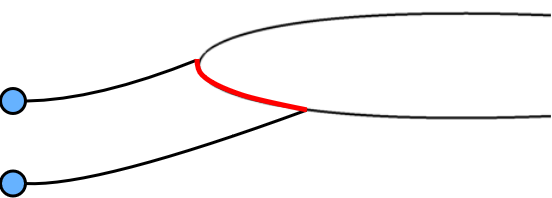
\includegraphics[width=.31\textwidth]{FIGURES/LAGRANGIAN_ARTICLE/FlowTube.png}
    \label{fig:flowTube}
    }%
    \subfloat[Local Flow Tube.]{%
    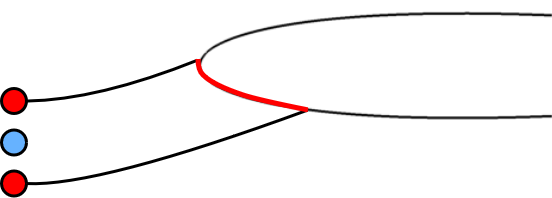
\includegraphics[trim={0cm 0cm 0cm 0cm},clip,width=.31\textwidth]{FIGURES/LAGRANGIAN_ARTICLE/LocalFlowTube.png}
    \label{fig:localFlowTube}
    }%
    \subfloat[\centering Pathological case for the collection efficiency.]{%
    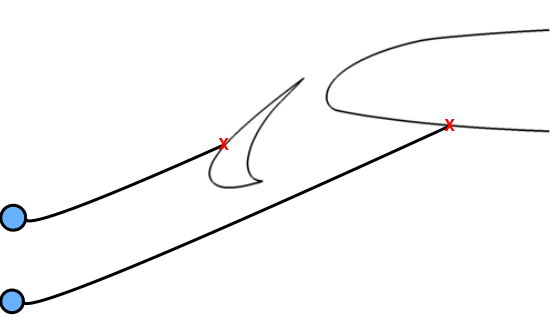
\includegraphics[trim={0cm 0cm 0cm 0cm},clip,width=.31\textwidth]{FIGURES/LAGRANGIAN_ARTICLE/ExtremeCase.png}
    \label{fig:extremeCase}
    }%
    \caption{Collection Efficiency computations. Primary and auxiliary droplets are represented in blue and red respectively.}
    \label{fig:collectionEfficiencyMethods}
\end{figure}

To address these challenges, a technique proposed in \cite{xie2020robust} introduces the computation of two additional auxiliary trajectories for each droplet , therefore creating a local flow tube for each droplet. The first issue is resolved by releasing the auxiliary trajectories in close proximity to the primary ones by a factor of : $dy \approx O(10^{-8}c_{\text{ref}})$, where $c_{ref}$ is the reference length of the geometry. The latter method increases the likelihood of droplets impacting the same geometric component in complex configurations.

Once all droplet trajectories (both primary and auxiliary) are computed, the corresponding collection efficiencies are determined. The final step is to transfer the local Lagrangian data to the cell-centered framework of the solver. Since multiple droplets can impact the same surface face, and to seamlessly integrate the Lagrangian solver within the CHAMPS framework, a weighted face average is applied during post-processing to assign a single $\beta_i$ value to the impacted surface cell as presented in Eq. \ref{eq:betaEqWeights}. The weighting $\omega_{i,d}$ for each droplet is based on the inverse square of the distance between the face center and the droplet’s impact position.

\begin{equation}
    \beta_i =  \frac{\sum \beta_{i,d} \cdot \omega_{i,d}}{\sum \omega_{i,d}}
    \label{eq:betaEqWeights}
\end{equation}

In 3D simulations, efficiently covering all surface faces without significantly increasing the droplet count is challenging. This issue can be alleviated by expanding the influence zone of each droplet. Using the available gradient stencil, neighboring boundary faces can be easily identified and also influenced by a droplet impact, extending its coverage area. Figure ~\ref{fig:impact} presents an example of a wind tunnel simulation around an airfoil, highlighting the difference in the impacted area for the same number of simulated droplets. Elements impacted by at least one droplet are shown in yellow (Fig. ~\ref{fig:impactwo}). In Fig.~\ref{fig:impactw}, the expanded impact zone is clearly visible, with previously unaffected elements in Fig.~\ref{fig:impactwo} now included.
    
\begin{figure}[htp] 
    \centering
    \subfloat[Without considering neighboring elements.]{%
        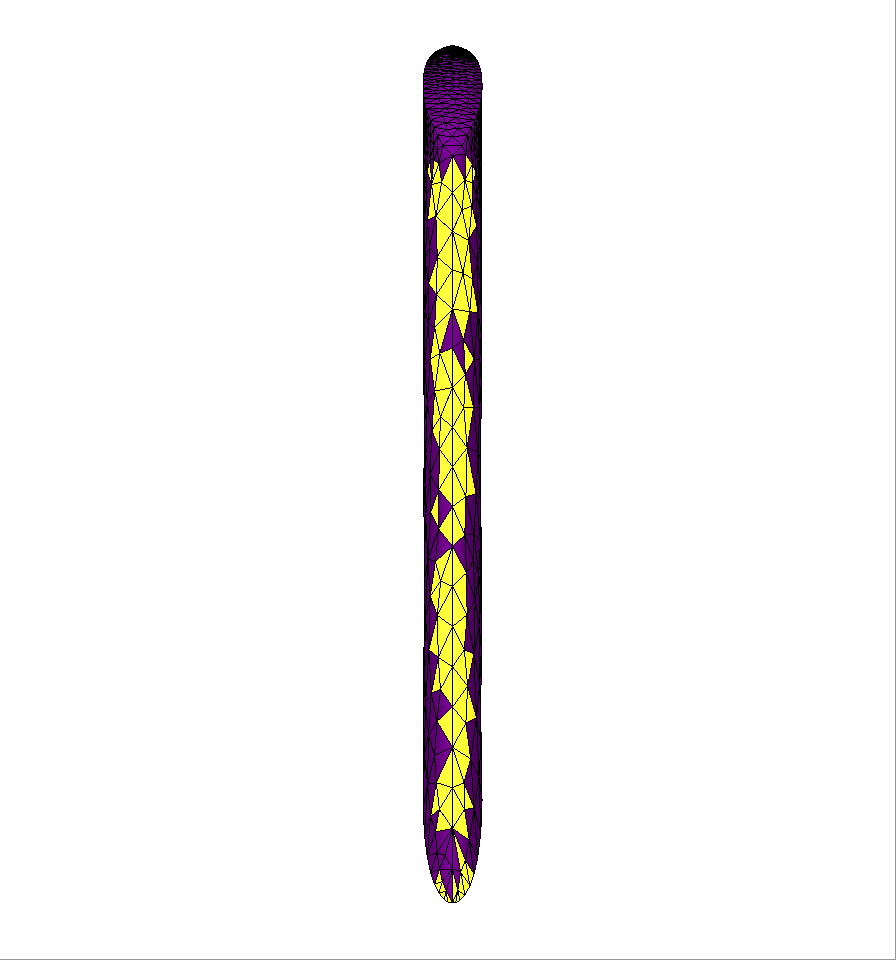
\includegraphics[trim={1cm 1cm 1cm 1cm},clip,width=0.45\textwidth]{FIGURES/LAGRANGIAN_ARTICLE/impactZoneWO.png}%
        \label{fig:impactwo}%
        }%
    \subfloat[With considering neighboring elements.]{%
        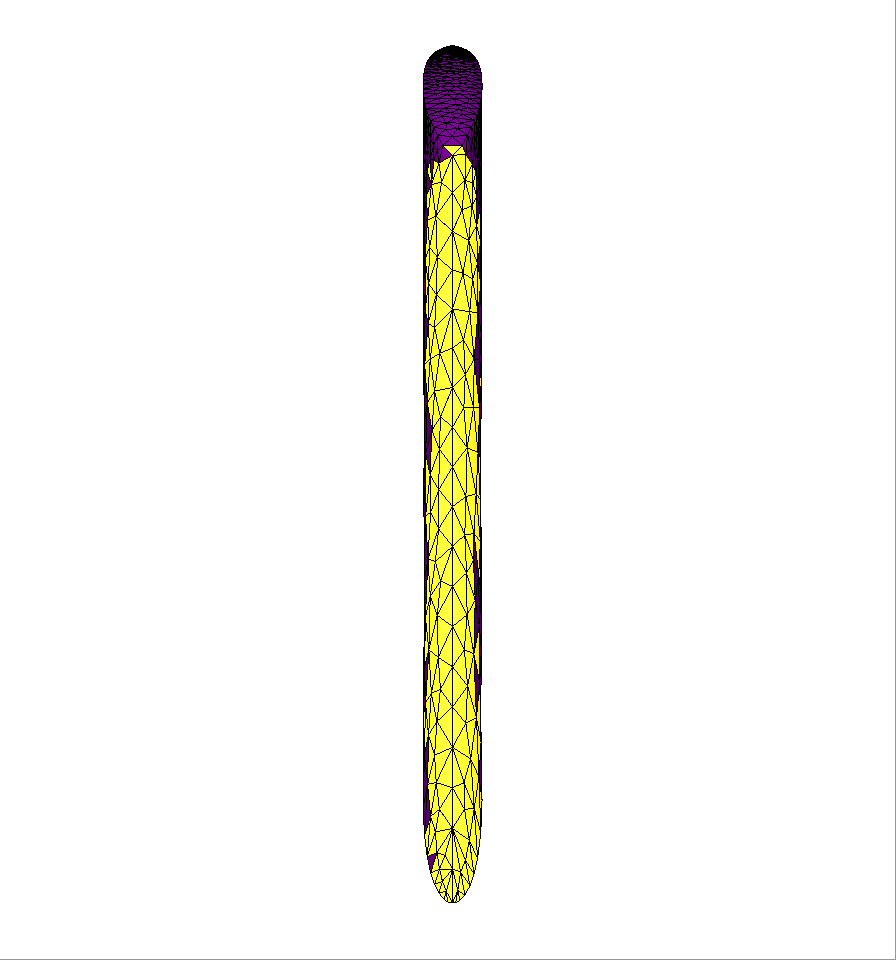
\includegraphics[trim={1cm 1cm 1cm 1cm},clip, width=0.45\textwidth]{FIGURES/LAGRANGIAN_ARTICLE/impactZoneW.png}%
        \label{fig:impactw}%
        }%
    \caption{Impact zone effect: Yellow-colored cells indicate at least one droplet impact, while purple-colored cells signify no impact.}
    \label{fig:impact}
\end{figure}

\subsection{SuperCooled Large Droplets Effects Modeling}
\label{Sec:SLDEffects}
 Supercooled Large Droplet (SLD) studies have gained significant attention following the requirements outlined in Appendix O of the Federal Airworthiness Regulations (FAR). SLD effects, such as droplet splashing and bouncing, might enable droplets to reach areas without anti-icing mechanisms. This can result in the formation of ice ridges, potentially causing flow separation and premature stalling of the aircraft. Another notable effect is droplet deformation due to shear stress in the flow, which alters the droplet’s shape, modifies its drag coefficient, and consequently change its trajectory course. The study of SLD ice accretion is challenging on both experimental and numerical fronts. Experimentally, obtaining reliable data is difficult, time-intensive, and expensive. References \cite{papadakis1999experimental, papadakis2003experimental, papadakism2004water} provide extensive datasets on SLD impingement distribution and ice shape characteristics.


 SLD behavior differs fundamentally from that of smaller supercooled droplets. Due to their larger diameters ($> 50 \mu m$ \cite{faa2010engine}), SLDs exhibit greater inertia and are less influenced by the flow, resulting in a higher likelihood of surface collision. Additionally, their geometric flexibility and susceptibility to deformation further distinguish them. As SLDs travel downstream, aerodynamic forces induce an uneven pressure distribution across their surface. When these forces exceed the capacity of interfacial and viscous forces to maintain a spherical shape, the droplets undergo deformation or even breakup (Fig. \ref{fig:DropletDeformation}). Consequently, droplets transition from a spherical to a nonspherical form, affecting both their trajectory and the volume of deposited water. However, except in freezing drizzle conditions, the impact of these phenomena is generally limited, as noted by \cite{trontin2016revisited}. In this study, droplet deformation is considered by adjusting the drag coefficient as proposed by \cite{clift2005bubbles}, while droplet breakup is not accounted for. The drag coefficient is obtained by blending spherical and oblate-disk correlations as a function of the droplet Reynolds and Weber numbers, as reported in Eq. \ref{eq:CdBlend} and \ref{eq:CdWeight}. Both $C_{D,\mathrm{sphere}}$ and $C_{D,\mathrm{disk}}$ are functions of the droplet Reynolds number and are taken from \cite{clift2005bubbles}.

\begin{equation}
C_D = (1-f)\,C_{D,\mathrm{sphere}} + f\,C_{D,\mathrm{disk}}
\label{eq:CdBlend}
\end{equation}

\begin{equation}
f = 1 - \left(1 + 0.07\sqrt{\mathrm{We}}\right)^{-6}
\label{eq:CdWeight}
\end{equation}

\begin{figure}[htp] 
    \centering
    \subfloat[Droplet Deformation.]{%
        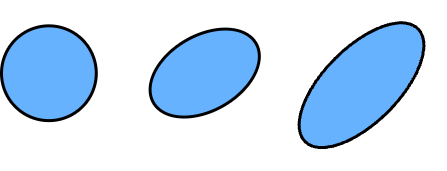
\includegraphics[width=0.45\textwidth]{FIGURES/LAGRANGIAN_ARTICLE/DropletDeformation.png}%
        \label{fig:DropletDeformation}%
        }%
    \subfloat[Droplet splashing.]{%
        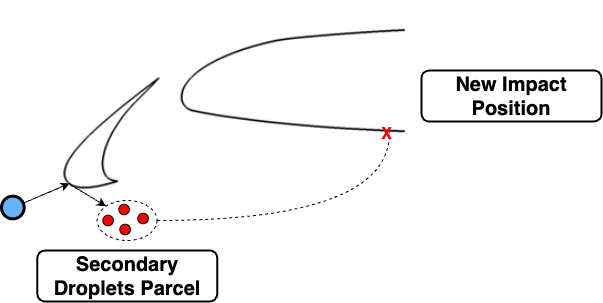
\includegraphics[width=0.45\textwidth]{FIGURES/LAGRANGIAN_ARTICLE/dropletSplashing.png}%
        \label{fig:DropletSplashing}%
        }%
    \caption{Droplet Phenomena.}
    \label{fig:DropletPhenomena}
\end{figure}

Droplet-wall interactions are particularly complex within the SLD regime. Unlike smaller droplets that tend to fully deposit on the surface, larger droplets often fragment into secondary droplets upon impact, as demonstrated in experiments \cite{cossali1999impact,rein1993phenomena,alzaili2011experimental,vanzante2007database} and illustrated in Fig. \ref{fig:DropletSplashing}. This fragmentation extends the impingement limits by enabling secondary droplet re-impingement, while lowering the peak collection efficiency. This behavior is influenced by droplet characteristics such as diameter, velocity, impact angle, density, viscosity, and surface tension, which are described using non dimensional numbers like Reynolds, Weber, and Ohnesorge numbers.

Numerically, simulating droplet impacts requires high-resolution meshes to capture interactions at the droplet scale. Methods like Volume of Fluid (VOF) \cite{hirt1981volume} and Moment of Fluid (MOF) \cite{lian2014numerical} have been used for this purpose. However, due to the large number of droplets involved in ice accretion simulations, these methods are computationally prohibitive with current hardware capabilities. Instead, semi-empirical models calibrated against experimental data are commonly employed. These models introduce the mass loss coefficient $f_m$ (or the sticking rate $\epsilon$) to account for the mass loss due to droplet splashing, directly influencing the initially computed collection efficiency $\beta_{i, \, 0}$ as expressed by:  

\begin{equation}
    \beta_{i, \, final} = (1.0 - f_m) \, \beta_{i, \, 0} 
\end{equation}

\begin{equation}
    \beta_{i, \, final} = \epsilon \, \beta_{i, \, 0} 
\end{equation}

\noindent Table \ref{tab:splashing_Models} summarizes the splashing models implemented in CHAMPS \cite{laroche2021development}. Wright et al. \cite{wright2004semi} enhanced their splashing model by incorporating the impact angle into the splashing parameters and mass loss formula. Their results show that splashing is less likely when droplets impact perpendicular to the wall and more pronounced near impingement limits. The model was calibrated by comparing simulated water collection efficiency with experimental data to ensure accuracy across a wide range of cases. Similarly, Trontin et al. \cite{trontin2016revisited} used sub-functions to represent the mass loss rate as a function of incident angle and kinetic energy. By comparing their numerical results with experimental data, they fine-tuned the parameters to improve model precision. Details regarding the models parameters can be found in the Appendix \ref{app:sldModels}. The effects of both models on the collection efficiency will be examined in greater detail in Section~\ref{sec:Results}.

% Please add the following required packages to your document preamble:
% \usepackage{multirow}
\begin{table}[htb!]
\centering
\caption{SLD Splashing Models}
\label{tab:splashing_Models}
\begin{tabular}{cc}
\hline
\hline
Literature Reference &
Mass Loss Coefficient \\ \hline\hline
\\
Wright et al. \cite{wright2004semi} &
$0.7 (1.0 - sin(\theta_0)) [1.0-e^{-0.0092(K_M - 200.0)}]$ \\ \\

\\
Trontin et al. \cite{trontin2016revisited} &
$ 1.0 - g(\frac{\theta}{\theta_c})f(\frac{K_c-K_0}{K_0})$\\ \\
\hline
\hline
\end{tabular}
\end{table}

As previously mentioned, depending on the impact conditions, droplet splashing on the surface leads to both mass deposition on the surface and the re-injection of smaller droplets into the flow (Fig. \ref{fig:DropletSplashing}). Ongoing studies are currently exploring the dynamics following droplet splashing on the surface, with current models offering limited insight into this phase. For example, \cite{wright2004semi} provides post-impact variables that enable the simulation of secondary droplets resulting from splashing, as shown in Eq. \ref{eq:postImpactVelocities} for post-impact velocities and Eq. \ref{eq:postImpactDiameter} for post-impact diameter. In CHAMPS, once all droplet trajectories are simulated and the sticking rate or mass loss is calculated for each droplet, the secondary droplets are modeled as a single parcel containing the mass from the point of impact. This approach remains a simplification since the SLD models listed in Table~\ref{tab:splashing_Models} do not provide detailed information on the nature of splashing. The secondary droplets are injected at the same boundary face where the impacts have occurred.

\begin{equation}
\begin{split}
    u_{n,\, post \, impact} = u_{n,\, impingement} (1.075 - 0.0025 \, \alpha_{impingement}) \\
    u_{t,\, post \, impact} = u_{t,\, impingement} (0.300 - 0.0020 \, \alpha_{impingement})
\end{split}
\label{eq:postImpactVelocities}
\end{equation}

\begin{equation}
    \frac{D_{new}}{D} = exp(-0.0281 \, K_M)
\label{eq:postImpactDiameter}
\end{equation}

\noindent The secondary droplets parcel is then tracked until the next impact position. This raises the question of how to properly incorporate the secondary droplets re-impingement contribution into the overall collection efficiency calculation. One approach could be to add the average contribution of all the secondary droplets impacting a given face, as expressed in Eq. \ref{eq:splashingIncluded}.

\begin{equation}
\beta_{final} = \epsilon \, \beta_{i, \, 0} + \frac{\sum \beta_{i, \, sd} \cdot \omega_i}{\sum \omega_i}
\label{eq:splashingIncluded}
\end{equation}

\noindent where $\omega_i$ are weights based on the distance between the new position of impact and the center of the corresponding face and $\beta_{i, \, sd} = f_m \, \beta_{i, \, d}$ is the loss in the collection efficiency from the first impact position. Another approach would be to normalize the secondary droplets contribution using Eq. \ref{eq:normalizedContribution}: 

\begin{equation}
    \beta_{Re-Impingement} = \frac{ m_{sd} \cdot (\boldsymbol{u_{sd}} \cdot \boldsymbol{n})/ A_s}{m_\infty \cdot  u_\infty /  A_\infty} 
    \label{eq:normalizedContribution}
\end{equation}

\noindent where $m_{sd}$ is the mass contained in the secondary droplet parcel, $\boldsymbol{u_{sd}}$ is the parcel velocity at the new impact position, $A_\infty$ is the area of the seeding grid, $A_s$ is the area of the facet on the geometry and $m_\infty$ is the initial injected droplet mass upstream. The latter can be directly added to $\beta_{final}$ of the boundary face. This latest approach is adopted in CHAMPS as it provides a more natural basis for normalizing the collection efficiency.

\subsection{Hybrid Eulerian-Lagrangian Solver}
Since SLD effects are Lagrangian in nature, they are challenging to implement in an Eulerian solver, particularly when modeling droplet splashing. The initial attempt by \cite{bilodeau2016numerical} involved switching boundary conditions to in-flow boundaries for splashed faces. In their work, a preliminary simulation is carried out to determine initial deposition. Boundary faces identified as splashed were then tagged and clustered based on specific metrics. As dual boundary conditions cannot be applied simultaneously, subsequent simulations were carried out for each cluster of boundary faces. The goal was to treat these faces as in-flow boundaries, injecting the appropriate amount of water droplets into the volume field to account for the re-injection. However, this approach proved computationally expensive, as it required additional simulations for numerous faces. A more recent approach by \cite{catalano2023modelling} addressed this issue by simulating all splashed faces simultaneously, assuming that water would not re-impinge on these faces. While this may apply in some cases, it cannot be guaranteed for complex configurations.

A recent technique by \cite{bellosta2023lagrangian} involved simulating the secondary droplets from splashing as Lagrangian droplets. This approach combined the efficiency of the Eulerian model for the initial deposition phase with the precision of the Lagrangian solver for tracking secondary droplets, thereby reducing the computational cost associated with simulating a large number of droplets.

The present work builds on this technique to enhance the capabilities of CHAMPS's Eulerian solver. The Eulerian solver is used to compute the initial deposition and apply splashing models to estimate the mass loss. For each splashed boundary face, a parcel of Lagrangian droplets is seeded and tracked using the Lagrangian method. The contribution of re-impingement is accounted by using Eq. \ref{eq:splashingIncluded}.

\subsection{Parallelism}
The droplet solver in CHAMPS is implemented in Chapel, a high-level open source parallel programming language designed for scalable high performance computing \cite{parenteau}. CHAMPS employs a domain decomposition strategy in which the computational grid is partitioned into mesh partition objects, each corresponding to a spatial subdomain and mapped directly to a computational rank. This design ensures a one-to-one correspondence between mesh partitions and MPI ranks, enabling distributed-memory parallelism while allowing users to adjust the partitioning according to available resources. Load balancing is achieved by partitioning both the flow and droplet seeding grids using the METIS algorithm \cite{karypis2003parmetis}, ensuring that computational work is evenly distributed. Special care is taken to avoid redundant droplet computations at zone interfaces by assigning shared droplets to the lowest zone ID. Intra-node communication overhead is minimized via local lightweight mesh copies shared among ranks on the same node, leveraging OpenMP-like parallelism to exploit shared-memory architectures. This hybrid MPI–OpenMP-like approach reduces inter-node communication costs while maintaining scalability across large distributed systems, thus enabling efficient tracking of large droplet populations within the Lagrangian framework.


\section{Results \& Discussions}
\label{sec:Results}

One of the primary focus of this study lies in the validation of Lagrangian droplet trajectory computations and the SLD implementation, primarily through the computed collection efficiency $\beta$. This metric is compared with previously validated Eulerian results in CHAMPS \cite{bourgault2019ice} for the droplet trajectory part. Additionally, the impact of SLD effects on the collection efficiency is analyzed using the models previously introduced. The cases presented in Table \ref{tab:results} are sourced from both the first and second Ice Prediction Workshop (IPW1-2, \cite{laurendeau2022summary, laurendeau2024summary}) and the fifth edition of the Highlift Prediction Workshop (HLPW5). The Ice Prediction Workshop (IPW) is a series of international initiatives organized by the American Institute of Aeronautics and Astronautics (AIAA) to evaluate and compare the performance of different numerical tools for aircraft icing prediction. It provides experimental datasets covering both 2D airfoils and 3D geometries under various icing conditions. The initial two cases are chosen to assess the implementation on a simplistic airfoil geometry, encompassing both two-dimensional and three-dimensional scenarios. The third case presents a hybrid configuration in a wind tunnel where there is a gap between the top of the airfoil and the tunnel. The final case examines the model performance and accuracy on a larger and more complex scale, with the Common Research Model (CRM). The flow simulations were carried out using CHAMPS RANS solver with Spalart Allmaras (SA) to model the turbulent viscosity. Results were extracted based on information and cut tools provided by the workshop committee when available. Eulerian results were obtained using an Upwind scheme with Van Albada limiter to compute the convective fluxes. Finally, all simulations were carried out using multiple bins distributions. The distributions provided by the IPW1-2 were utilized for the concerned cases. A Freezing Rain (FR) distribution from Appendix 0 is applied for the fourth case to simulate a more realistic scenario for such case. Usually poly-dispersed clouds are chosen due to the absence of a guarantee in experimental results regarding a single diameter size for all droplets. Depending on the experimental setup, a distribution of droplet diameters is provided, indicating the likelihood of each diameter using a cumulative density function. The collection efficiency $\beta_i$ for each diameter bin is computed sequentially, with each bin assigned a weight $\gamma_i$. At the end of the simulation, all contributions are summed using Eq. \ref{eq:betaTotal}:

\begin{equation}
    \beta_{i,total} = \sum_{n=1}^{N_{bins}} \beta_i * \gamma_i
    \label{eq:betaTotal}
\end{equation}

\begin{table}[ht]
\caption{ Cases parameters}
\hspace*{-2cm}
\begin{tabular}{cccccccc}
\hline \hline
CASE & Description & MVD[$\mu m$] & AOA[\textdegree]& Ma[-]& C$_{ref}$[inch] & T [K] &  Re[-]\\
\hline
IPW1 - 112 & NACA64A008 H-Tail & 92 & 6.0 & 0.23 & 37.65 & 280.0 & 5 $\cdot 10^6$ \\
\hline
IPW1 - 122 & Three Element Airfoil & 92 & 4.0 & 0.23 & 36.0 & 278.0 & 4.8 $\cdot 10^6$ \\
\hline
IPW2 - 1.3 & CRM Hybrid & 25 & 3.7 & 0.21 & 39.37 & 247.15 & 8.1 $\cdot 10^6$ \\
\hline
HLPW5 - 2.1 &  CRM Wing-Body & FR & 6.0 & 0.20 & 275.8 & 288.15 & 5.4 $\cdot 10^6$\\
\hline \hline
\end{tabular}
\label{tab:results}
\end{table}


\subsection{Scalability}
To evaluate the efficiency of the parallelization of the Lagrangian solver, Case IPW2 - 1.3 is selected as the benchmark. All the necessary simulations are conducted on the Digital Research Alliance of Canada Trillium cluster. Each node in this cluster is equipped with two sockets, each containing 2 AMD EPYC 9655 (Zen 5, 2.6 GHz), resulting in a total of 192 cores per node. Simulations are conducted using a minimum of 2 and a maximum of 16 nodes, with the node count doubling at each measurement point.

The flow conditions from the original workshop case are adopted. A single droplet diameter, corresponding to the Mean Value Diameter (MVD) of $25 \, \mu m$, is employed. A total of 12.8 million droplets are seeded for the benchmark. This choice is based on the number of droplets needed for convergence and ensured optimal load balancing across all nodes, facilitating a more accurate comparison of performance.

Unlike Eulerian simulations, where the iteration time correlates to solver efficiency, this metric is not directly applicable to Lagrangian solvers. This is because droplets may require different numbers of iterations to either impact the geometry or move past it. Consequently, the metric selected for comparison is the total computation time.

\begin{figure}[t]
\centering
    \subfloat[Solver Speed Up.]{%
        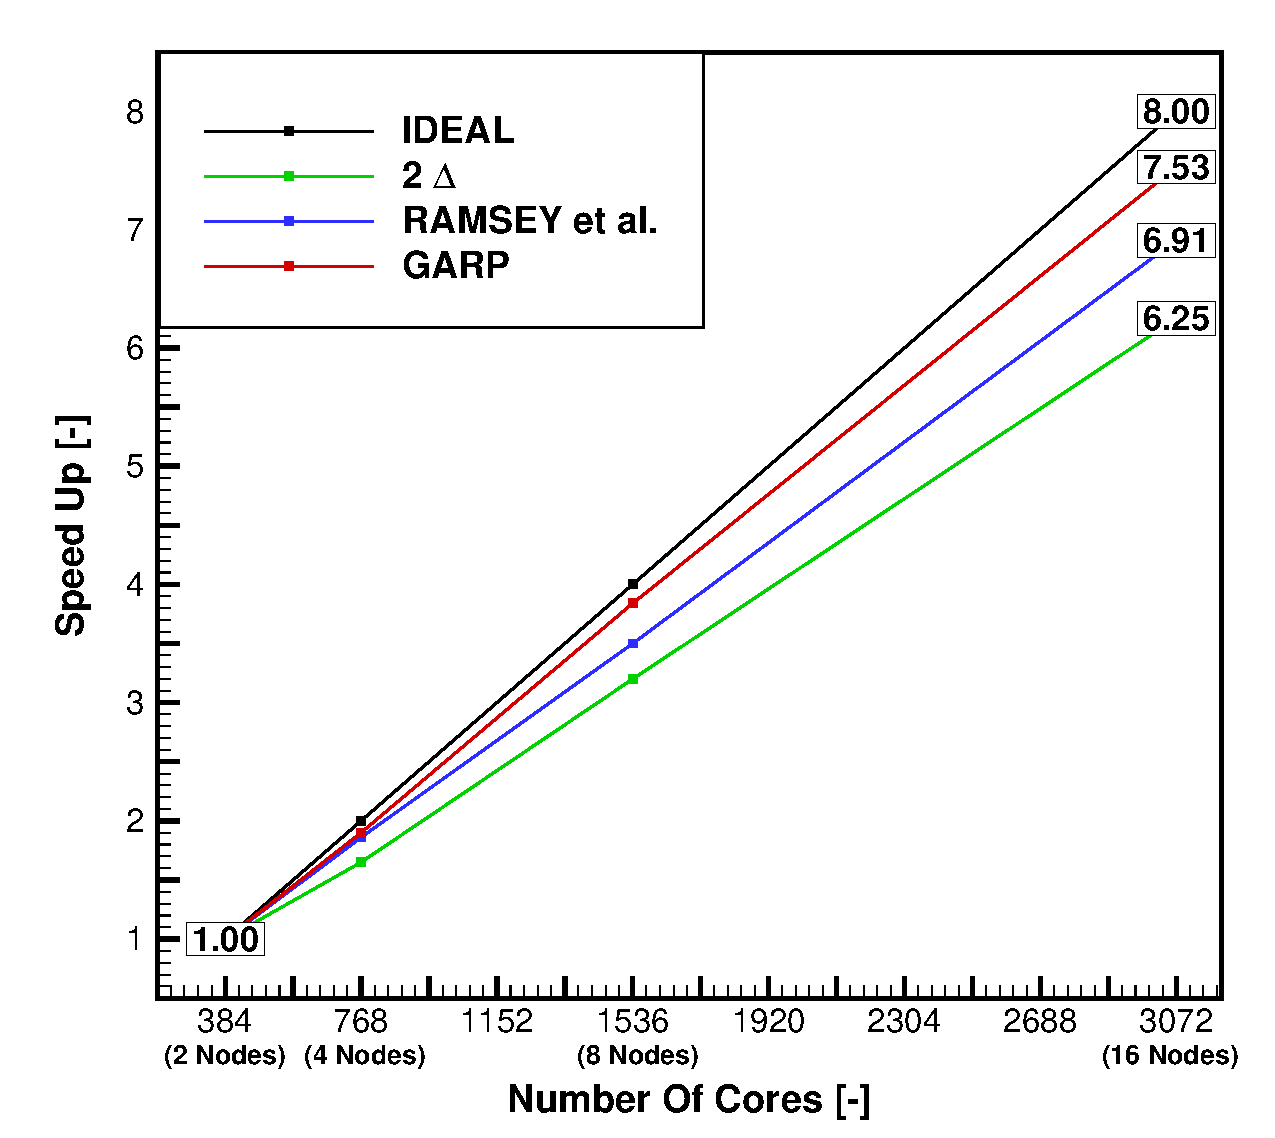
\includegraphics[trim={0cm 0cm 0cm 0cm},clip,width=0.48\textwidth]{FIGURES/LAGRANGIAN_ARTICLE/SpeedUp.eps}
        \label{fig:SolverSpeedUp}%
        }%
    \subfloat[Solver Efficiency]{%
        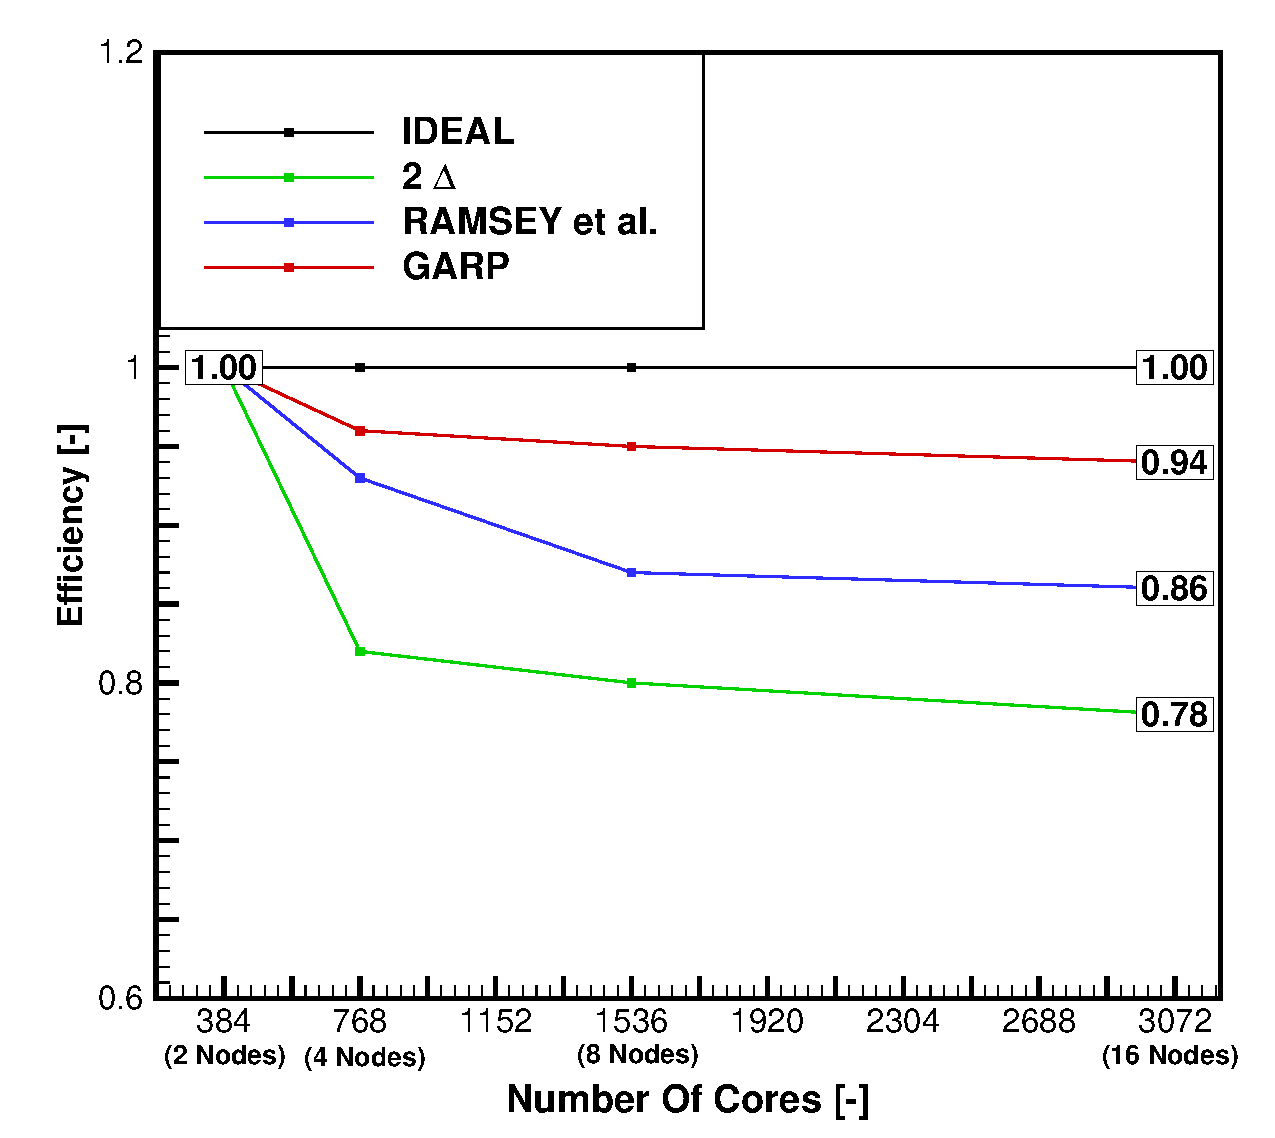
\includegraphics[trim={0cm 0cm 0cm 0cm},clip,width=0.48\textwidth]{FIGURES/LAGRANGIAN_ARTICLE/Efficiency.eps}
        \label{fig:SolverEfficiency}%
        }%
    \caption{Lagrangian Solver Scalability.}
    \label{fig:scalability}
\end{figure}

The computational speedup is determined using Eq.~\ref{eq:speedUp}, and the efficiency is computed using Eq.~\ref{eq:efficiency}. To account for the choice of two nodes as the baseline for comparison, a factor of 2 was included in the efficiency calculation. The results of this study are presented in Fig.~\ref{fig:scalability}. Results show only a $6\%$ loss in efficiency when using 16 nodes with the GARP technique, which demonstrates better scalability compared to both the method presented in \cite{Ramsey_2004} and two-triangle intersection methods. A contributing factor to GARP’s improved scalability is that it replaces the two-triangle split with a single, robust ray–patch intersection evaluation, reducing computational overhead and parallel-communication costs. It also involves substantially less branching than the method used in \cite{Ramsey_2004}, leading to more predictable memory access. Overall, the solver’s parallel performance aligns well with trends reported in the literature, confirming its robustness and computational efficiency on distributed-memory systems. 

The loss in efficiency can be associated with differences in droplet trajectories: for instance droplets reaching the leading edge of the geometry follow shorter paths than those reaching the trailing edge. While METIS effectively partitions the seeding grid to optimize load balancing, even small variations in trajectory execution times can degrade the performance of ranks handling droplets that traverse the full geometry. One potential solution is to refine the initial partitioning using ParMETIS \cite{karypis2003parmetis}. However, this requires precomputing additional droplet trajectories, which increases the overall computational cost.

\begin{equation}
    Speed \, Up = \frac{Simulation \, Time \, 2 \, Nodes}{Simulation \, Time \, N \, Nodes}
    \label{eq:speedUp}
\end{equation}

\begin{equation}
    \eta = 2 \cdot \frac{Speed \, Up}{ N \, Nodes}
    \label{eq:efficiency}
\end{equation}

\subsection{Case IPW1 - 112 : NACA64A008 Horizontal Tail }
Figure \ref{fig:Impinge} presents impingement results of Case IPW1 - 112. The geometry of the case is provided in Appendix~\ref{app:geometries}. Within Fig. \ref{fig:HTAILSINGLE}, the effects of extending the impact zone of a droplet become apparent. When examining identical droplet quantities, the Lagrangian solution without the extension reveals undesired oscillations, because the present work solves continuous equations, which are not expected to produce oscillations, unlike experimental measurements which contains discrete sets each with their own experimental uncertainty. The newly purposed enhancement gives smooth results, and more importantly the new collection efficiency matches the Eulerian results. Lagrangian trajectories exhibit similar outcomes when compared to Eulerian results for both single diameter (92 $\mu$m Fig. \ref{fig:HTAILSINGLE}) and using the diameter distribution provided by the workshop in Fig. \ref{fig:HTAILEULAG}. The use of diameter distributions affects collection efficiency, as shown in Fig.~\ref{fig:HTAILSINGLEVSDIST}. Results using a diameter distribution exhibit extended impingement limits (approximately 0.1 in difference in the surface distance on the lower surface), due to smaller droplets following the flow streamlines more closely. These droplets are less likely to impact near the stagnation point but have a higher probability of colliding farther downstream.


\begin{figure}[t]
\vspace{-1cm}
\centering
\hspace*{-0.5cm}
\subfloat[\centering Effect of droplet impact zone.]{%
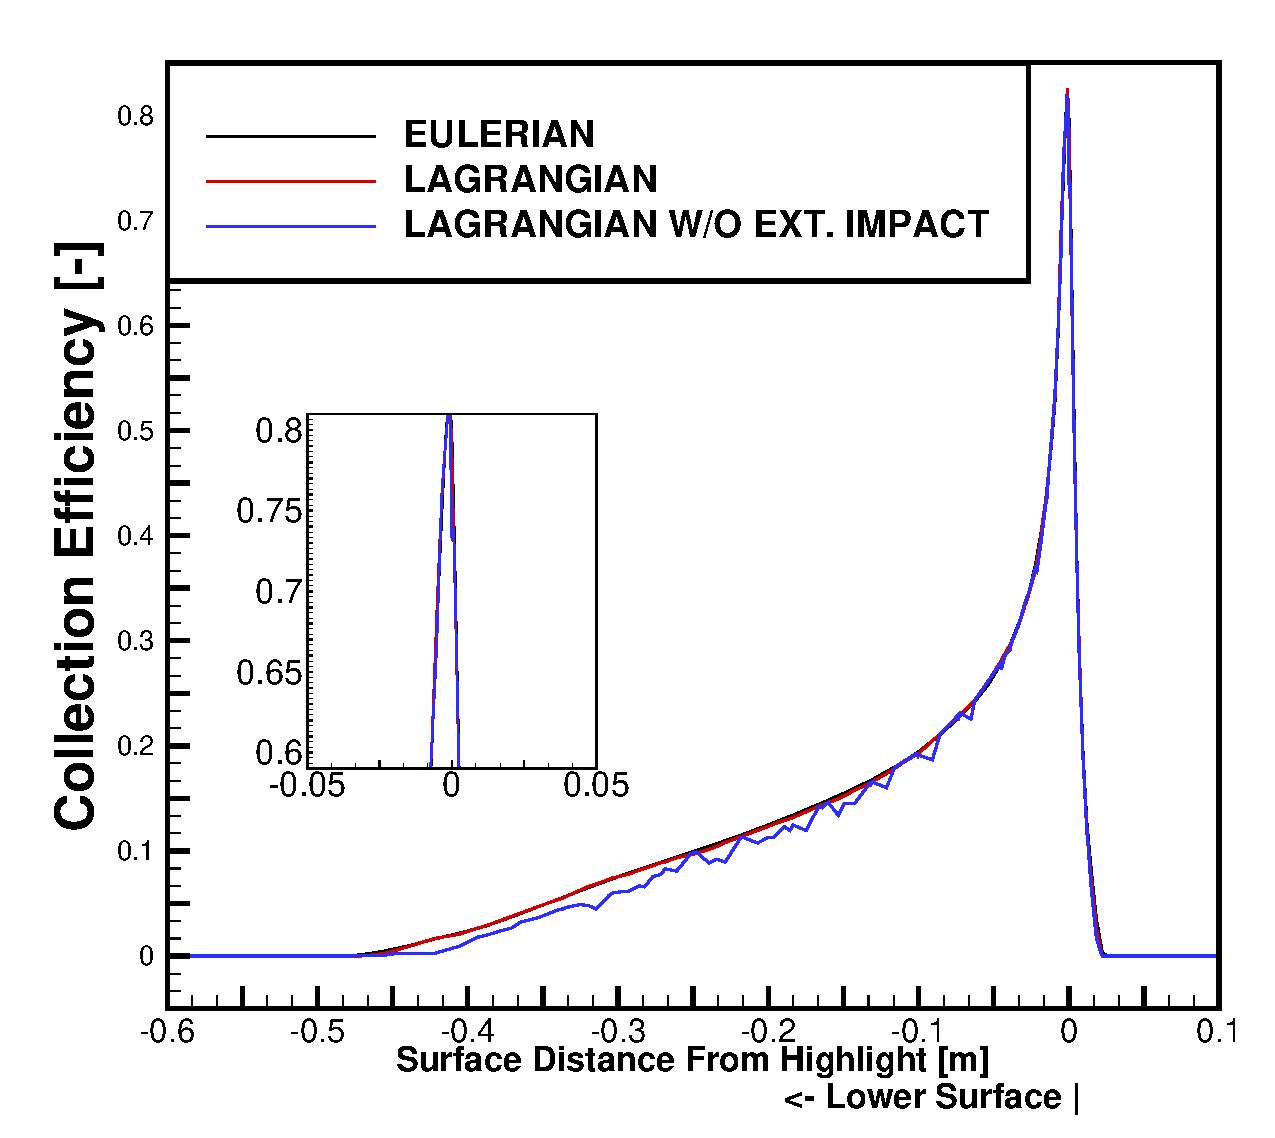
\includegraphics[width=0.49\textwidth]{FIGURES/LAGRANGIAN_ARTICLE/CASE_112_IMPACT_ZONE.eps}   
\label{fig:HTAILSINGLE}}
\subfloat[\centering Effect of droplet distribution on collection efficiency.]{%
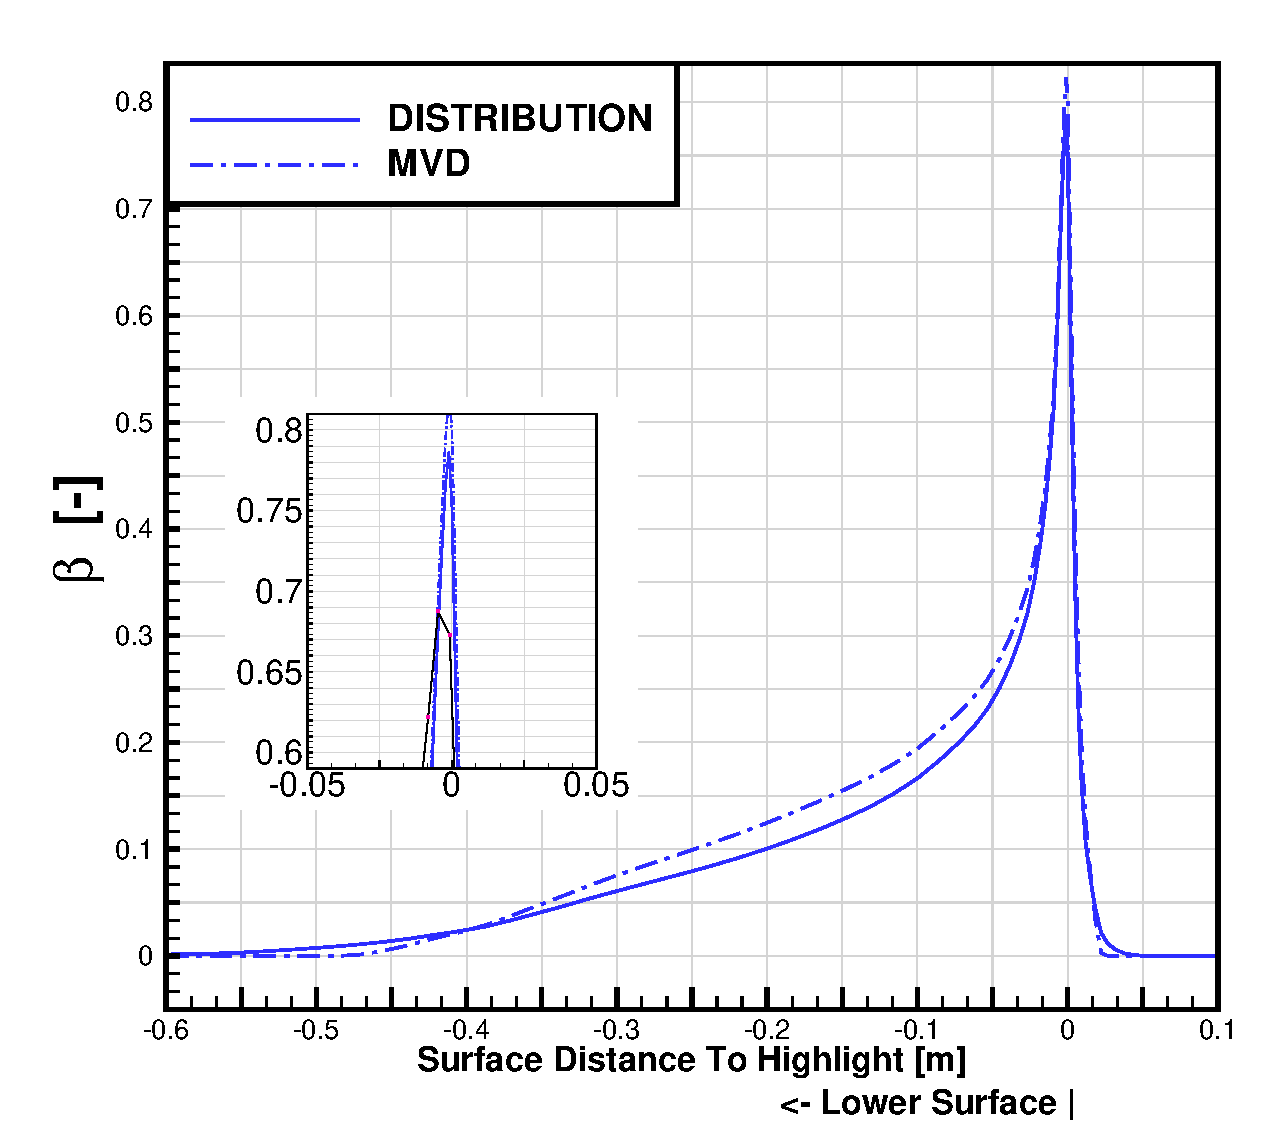
\includegraphics[width=0.49\textwidth]{FIGURES/LAGRANGIAN_ARTICLE/CASE_112_MVD.eps}
\label{fig:HTAILSINGLEVSDIST}%
}

\hspace*{-1cm}
\subfloat[\centering  Impingement results.]{%
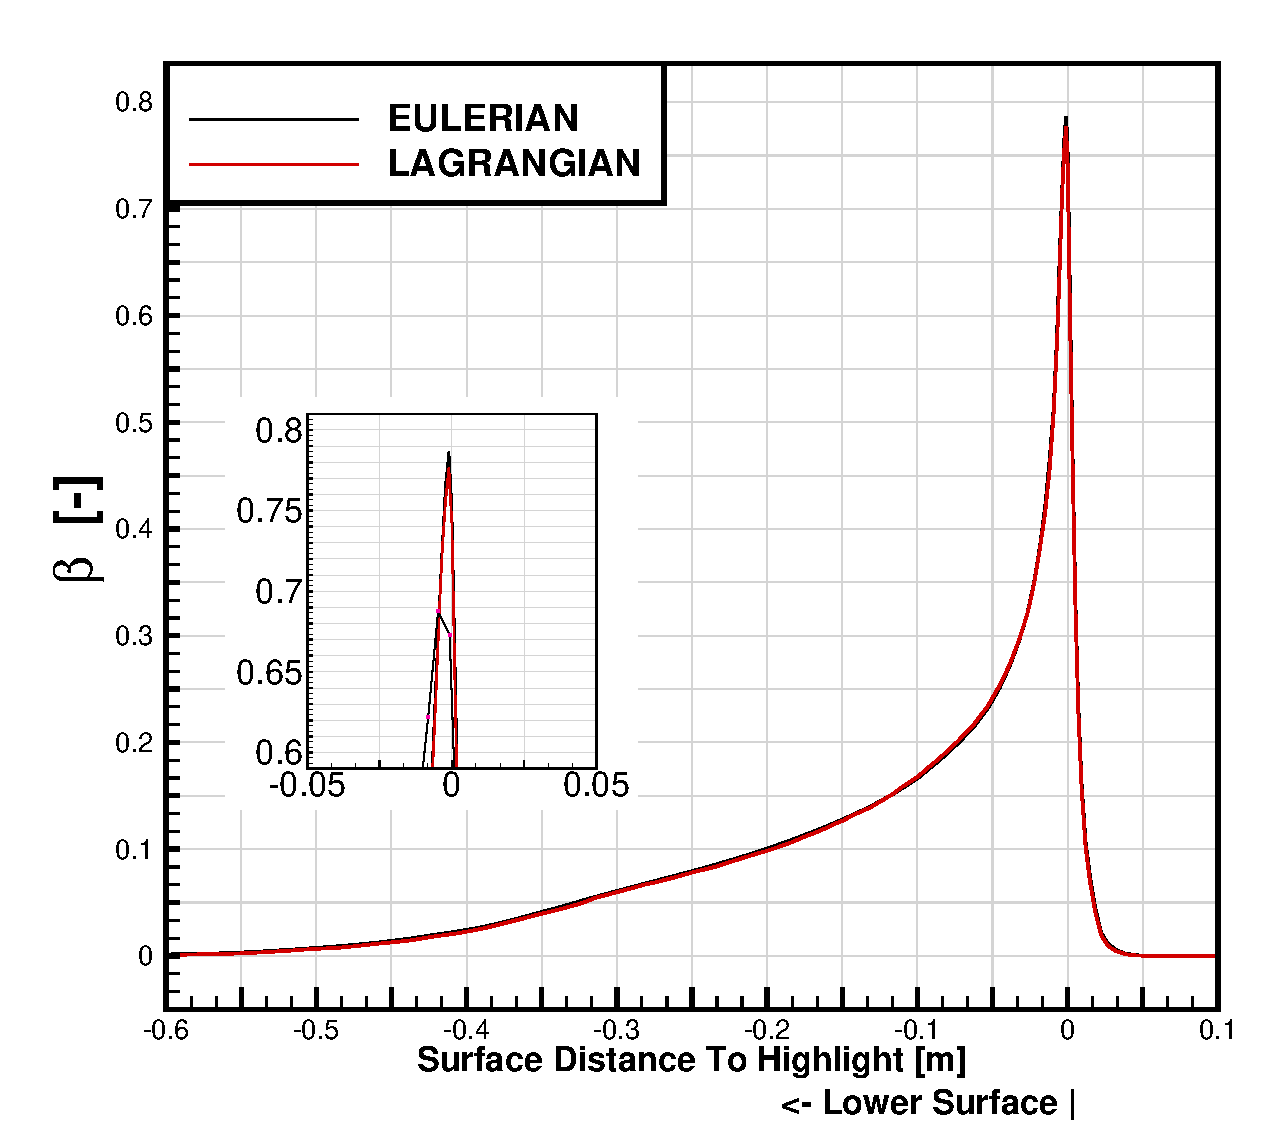
\includegraphics[width=0.49\textwidth]{FIGURES/LAGRANGIAN_ARTICLE/CASE_112_DISTRIBUTION.eps}
\label{fig:HTAILEULAG}%
}
\centering
\subfloat[\centering  SLD results.]{%
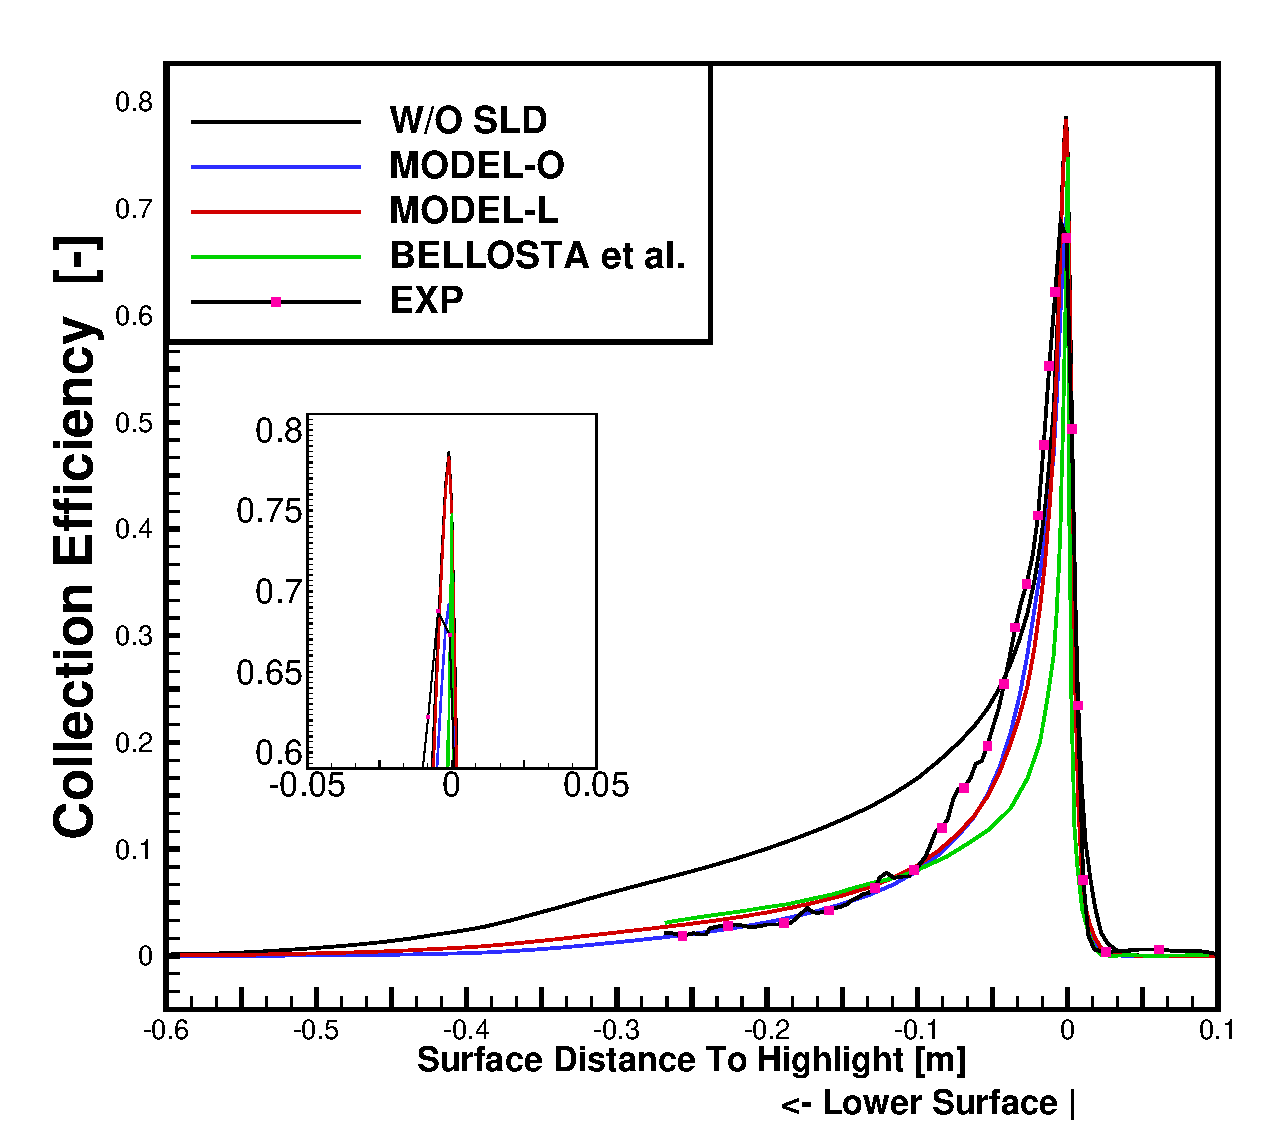
\includegraphics[width=0.49\textwidth]{FIGURES/LAGRANGIAN_ARTICLE/CASE_112_SLD.eps}
\label{fig:HTAILBETRA}%
}%
\caption{\centering Results for CASE IPW1 - 112.}
\label{fig:Impinge}
\end{figure}

The second objective to this study is to outline the SLD outcomes on the aforementioned cases (Table \ref{tab:results}). This serves the dual purpose of validating the implementation of the SLD models and examining the impacts of integrating such variables into consideration. The results consist of comparing the distribution $\beta$ for the previously presented SLD models in both formulations. Employing these approaches has a significant impact on the computed collection efficiency, by bringing its amplitude and limits closer to the experimental data. This is illustrated in Fig. \ref{fig:HTAILBETRA} when comparing with the experimental results of \cite{papadakism2004water}. Without considering the effects of SLD, the computed collection efficiency is significantly higher than the available experimental data. The model provided by \cite{wright2004semi} (denoted as "MODEL-L") is specifically engineered to minimize the SLD effects near the stagnation point and to gradually increase these effects when moving towards the impingement limits. This characteristic can be seen in its formulation: as the impact angle approaches 90\textdegree $\, $in this region, the mass loss coefficient is approximately zero, indicating that no splashing occurs when the impact angle is normal to the surface. However, further down the geometry, the mass loss effects become more apparent since the impact angle becomes more tangential to the surface. This results in the same solution as the one without SLD effects at the stagnation point, with a gradual decrease in $\beta$ thereafter.

On the other hand, the model provided by \cite{trontin2016revisited} (denoted as "MODEL-O") operates differently. This model assumes that near the stagnation point, when the impact angles are normal to the surface, the droplets should exhibit mass loss depending on their impact velocity. Higher velocities increase the likelihood of droplet splashing, thereby increasing the mass loss coefficient in this region. This approach provides a closer alignment with experimental data as shown in Fig. \ref{fig:HTAILBETRA}. Both models exhibit similar behavior as they move farther from the stagnation point, tending to accurately predict the impingement limits. CHAMPS results are also compared with the SLD data reported in \cite{bellosta2023lagrangian}, which employs the same SLD model as in \cite{wright2004semi} ("MODEL-L"). CHAMPS shows closer agreement with experimental observations, although a direct comparison is difficult given differences in flow conditions, mesh resolution, and other factors. A key distinction lies in the computation of the collection efficiency. In \cite{bellosta2023lagrangian}, a statistical approach (Eq. \ref{eq:betaEqFlux}) comparing the upstream water mass flux ($m_\infty u_\infty / A_\infty$) with the local surface flux ($\boldsymbol{u_d} \cdot \boldsymbol{n} / A_s$) is used:

\begin{equation}
    \beta = \frac{\sum m_{d} \cdot (\boldsymbol{u_d} \cdot \boldsymbol{n})/ A_s}{m_\infty u_\infty / A_\infty} 
    \label{eq:betaEqFlux}
\end{equation}

\noindent However, this method requires a significantly larger number of droplets to achieve comparable accuracy. In the present work, the local flow-tube technique is employed, yielding accurate estimates of the collection efficiency.


\subsection{Case IPW1 - 122 : Three Element Airfoil}
 Case IPW1 - 122 presents a configuration that is particularly challenging because of the re-circulation cove behind the Main element (Fig. \ref{fig:streamtraces}). Disparities emerge notably in the Main and Flap components of the geometry as was shown by most IPW1 participants (Fig. \ref{fig:MDA_MAIN_IPW1} - \ref{fig:MDA_FLAP_IPW1}). Fig. \ref{fig:MDA_SLAT_DISTRIBUTION}, \ref{fig:MDA_MAIN_DISTRIBUTION} and \ref{fig:MDA_FLAP_DISTRIBUTION}  show the results obtained in CHAMPS for both models using the diameter distribution provided by the workshop. The two models exhibit a good level of agreement. The Eulerian model tends to detect impingement towards the end of the main airfoil component on both sides of the geometry. This discrepancy arises from non-physical values observed for the droplet volume fraction, attributed to dispersion-induced oscillations. The prominence of the Slat component in collecting incoming droplets is apparent, due to its position at the forefront of the geometry. This trend is particularly pronounced on the pressure side, where the geometry is angled at a 4\textdegree $\,$ angle of attack, resulting in a greater accumulation of droplets. This configuration also influences the Main and Flap components, with minimal impingement observed on their suction side. Overall similar results can be observed between the two models. The slight difference between Eulerian and Lagrangian results can be related to dissipation from the Eulerian model, especially near the cove behind the main component as noted in \cite{blanchet2022conservative}. Ideally, these differences would diminish with mesh refinement as showcased in Appendix \ref{sec:VERIF_NACA}. 

\begin{figure}[h!]
\hspace*{0cm}
    \subfloat[Three Element Airfoil Geometry.]{%
    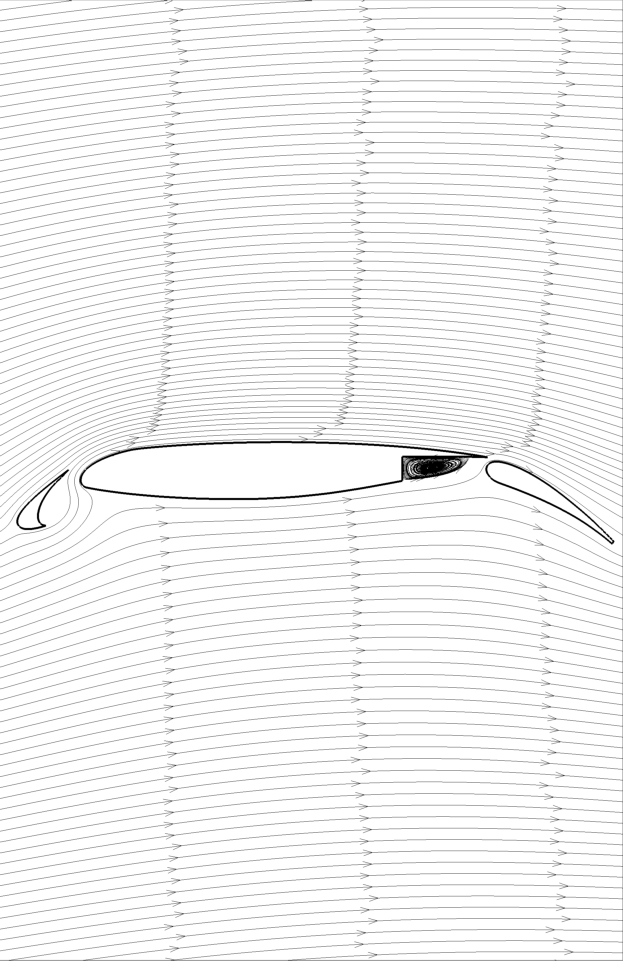
\includegraphics[trim={0cm 10.5cm 0cm 10.5cm},clip,width=0.6\textwidth]{FIGURES/LAGRANGIAN_ARTICLE/MDA_FLOW_FIELD.png}
    \label{fig:MDA_Geometry}%
    }
    \hspace*{0.1cm}
    \subfloat[\centering Recirculation zone in the cove of the main element.]{%
    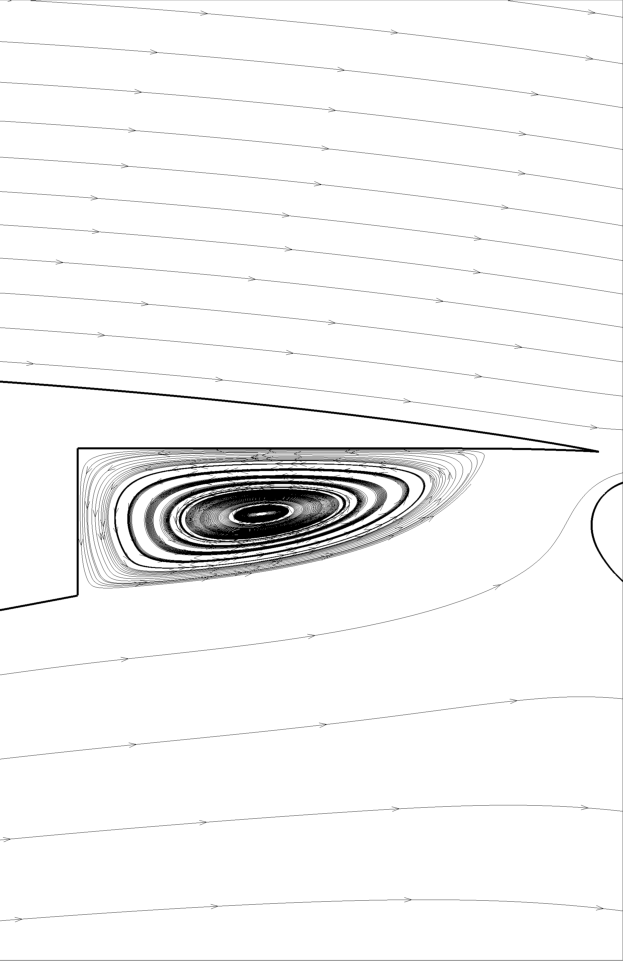
\includegraphics[trim={2cm 8cm 0cm 8cm},clip,width=0.4\textwidth]{FIGURES/LAGRANGIAN_ARTICLE/MDA_RECIRCULATION.png}
    \label{fig:streamtraces}%
    }
    \caption{Description of Case IPW1 - 122.}
    \label{fig:MDA_CASE_DESCRIPTION}
\end{figure}

\begin{figure}[h!]
\hspace*{-1cm}
% \subfloat[IPW1 results on the Slat.]{%
% \includegraphics[width=0.35\textwidth]{FIGURES/RESULTS/CASE_122/PARTICIPANTS/SLAT_PARTICIPANTS.png} \quad
% \label{fig:MDA_SLAT_IPW1}%
% }%
%\hspace*{-1cm}
\subfloat[Main component results.]{%
\includegraphics[trim={.1cm .1cm .1cm .1cm},clip,width=0.49\textwidth]{FIGURES/LAGRANGIAN_ARTICLE/CASE_122_MAIN_IPW1.eps}
\label{fig:MDA_MAIN_IPW1}%
}
\hspace*{0.5cm}
\subfloat[ Flap component results. ]{%
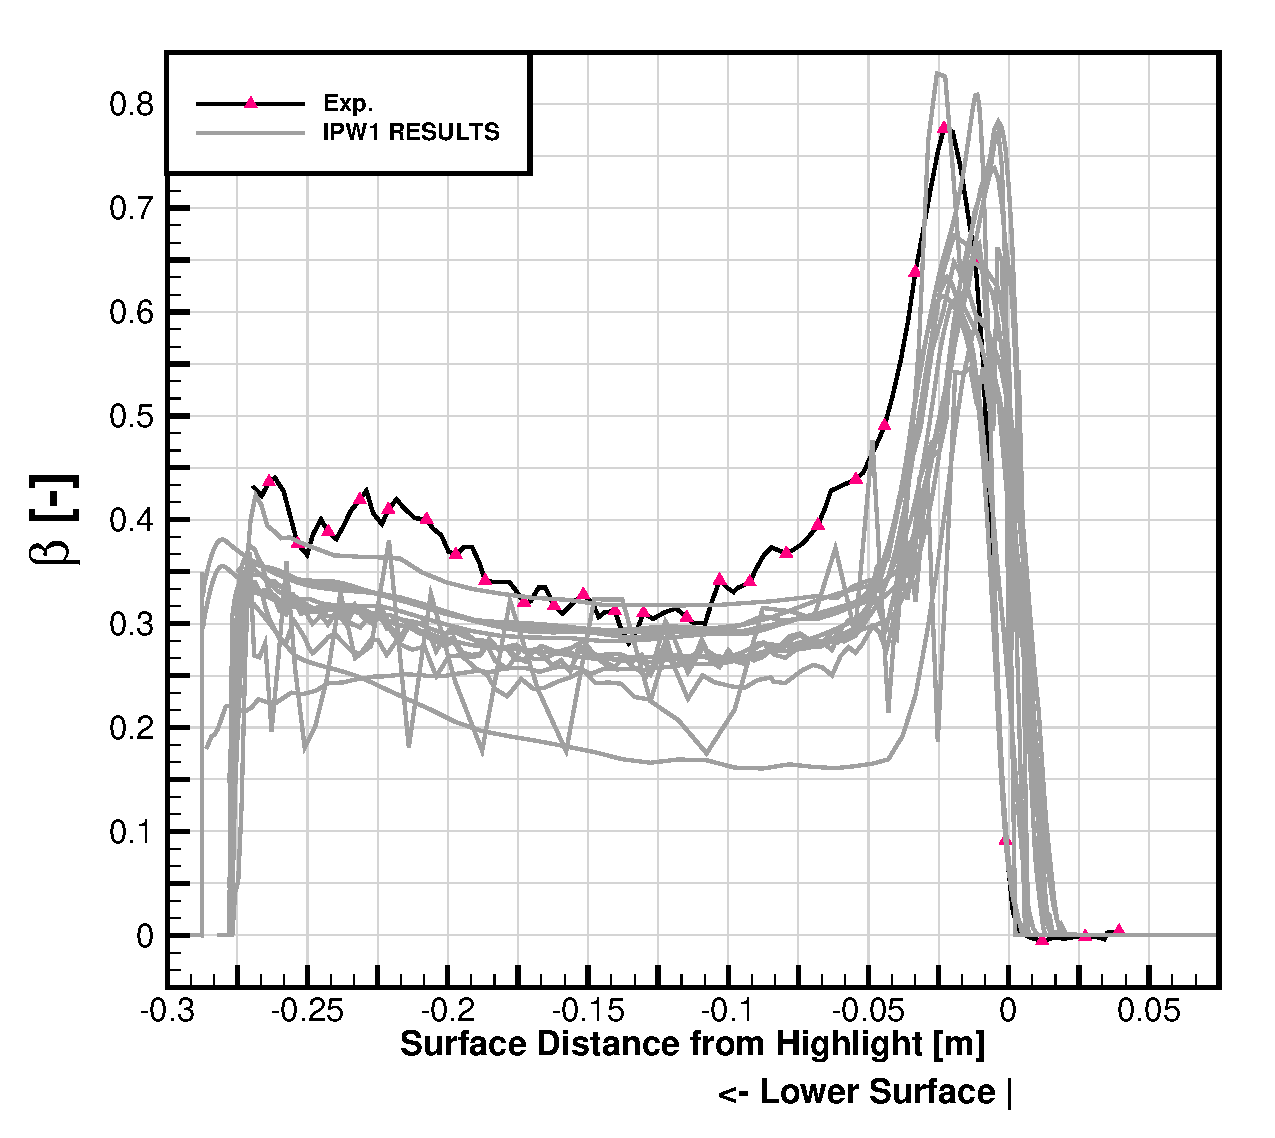
\includegraphics[trim={.1cm .1cm .1cm .1cm},clip,width=0.49\textwidth]{FIGURES/LAGRANGIAN_ARTICLE/CASE_122_FLAP_IPW1.eps}
\label{fig:MDA_FLAP_IPW1}%
}
\caption{Aggregated impingement results of all IPW1 participants for Case IPW1-122.}
\label{fig:MDA_Participants}
\end{figure}

 The SLD results are illustrated in Fig. \ref{fig:MDA_SLAT_SLD}, \ref{fig:MDA_MAIN_SLD} and \ref{fig:MDA_FLAP_SLD}. On the slat component of the geometry, the computations accurately predict the experimental collection efficiency, both in terms of peak values and impingement limits. On the main component, the collection efficiency is significantly underestimated. On the flap part of the geometry, the numerical simulations align more closely with the experimental results. The impingement limits are well predicted. However, the peak value for $\beta$ is underestimated for the same reason as the main component. When considering secondary droplet re-impingement using the method presented in Section \ref{Sec:SLDEffects} (denoted “MODEL-L w/ REIMP.”) on both the main component and the flap, an increase in the peak value of $\beta$ is observed, leading to a slightly better agreement with experimental data.

A similar trend is observed for the hybrid model (denoted “EUL. MODEL-L w/ REIMP. HYBRID”). The effect of re-injected Lagrangian droplets is particularly pronounced on the flap component, where the peak value increases compared to the baseline Eulerian model (denoted “EUL. W/O SLD”). A similar trend is observed across participants’ data and even in more recent results for this case \cite{bellosta2023lagrangian, moula2023icing}. This raises questions about the reliability of the re-injection model in predicting post-impact variables or/and the validity of the experimental results for this specific case.

\begin{figure}[h!]
\hspace*{-1cm}
\subfloat[Impingement results on the Slat.]{%
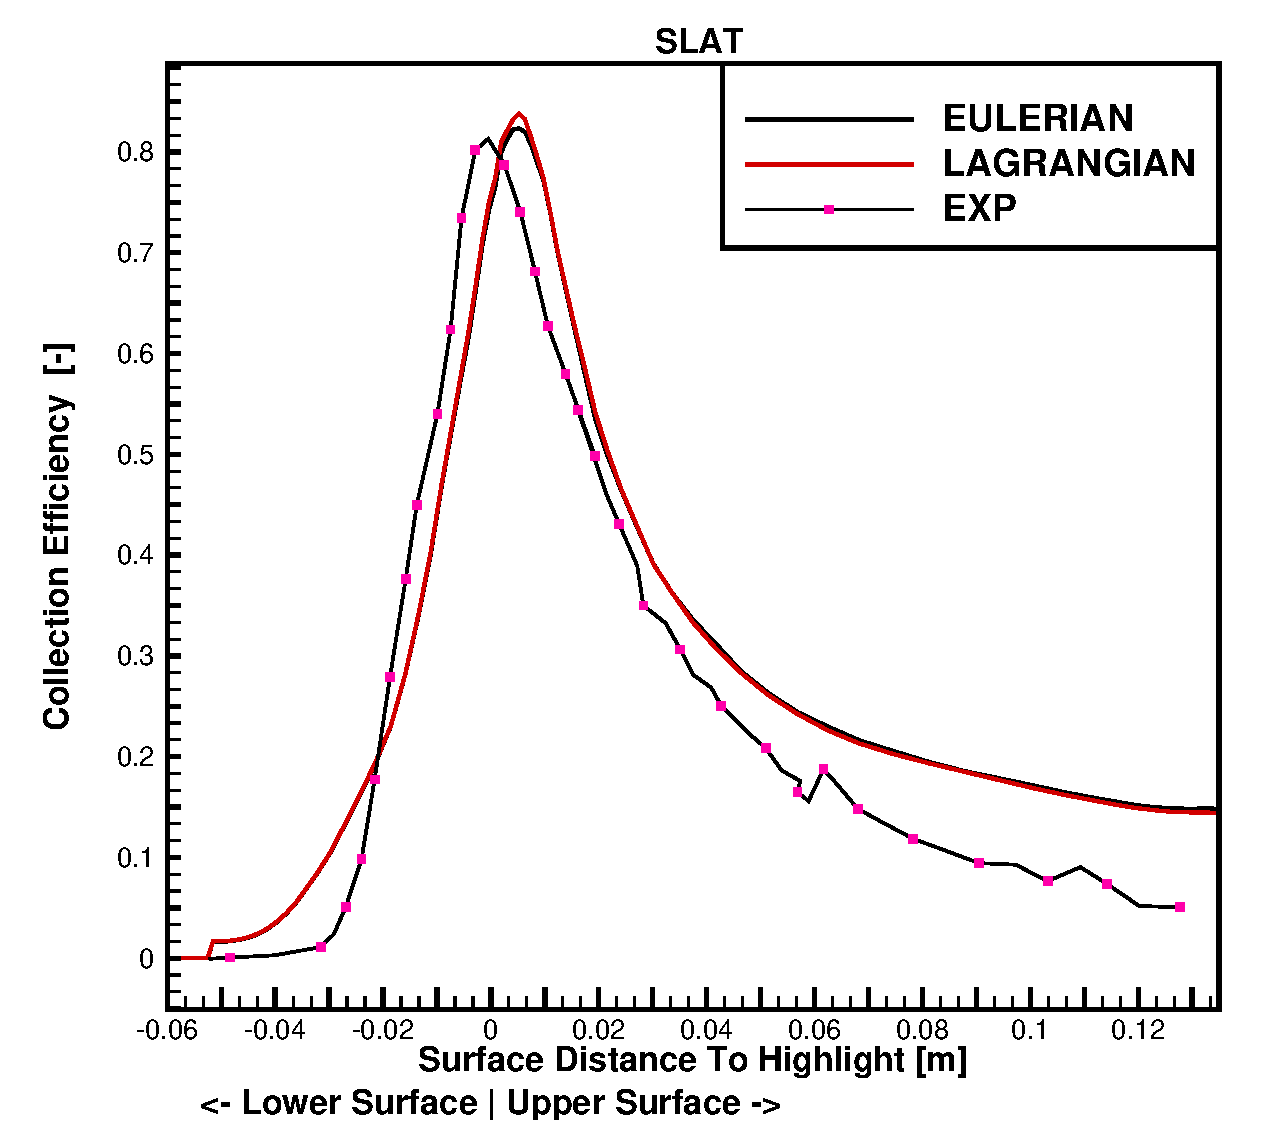
\includegraphics[width=0.325\textwidth]{FIGURES/LAGRANGIAN_ARTICLE/CASE_122_SLAT_DISTRIBUTION.eps} \quad
\label{fig:MDA_SLAT_DISTRIBUTION}%
}%
%\hspace*{-1cm}
\subfloat[\centering Impingement results on the Main.]{%
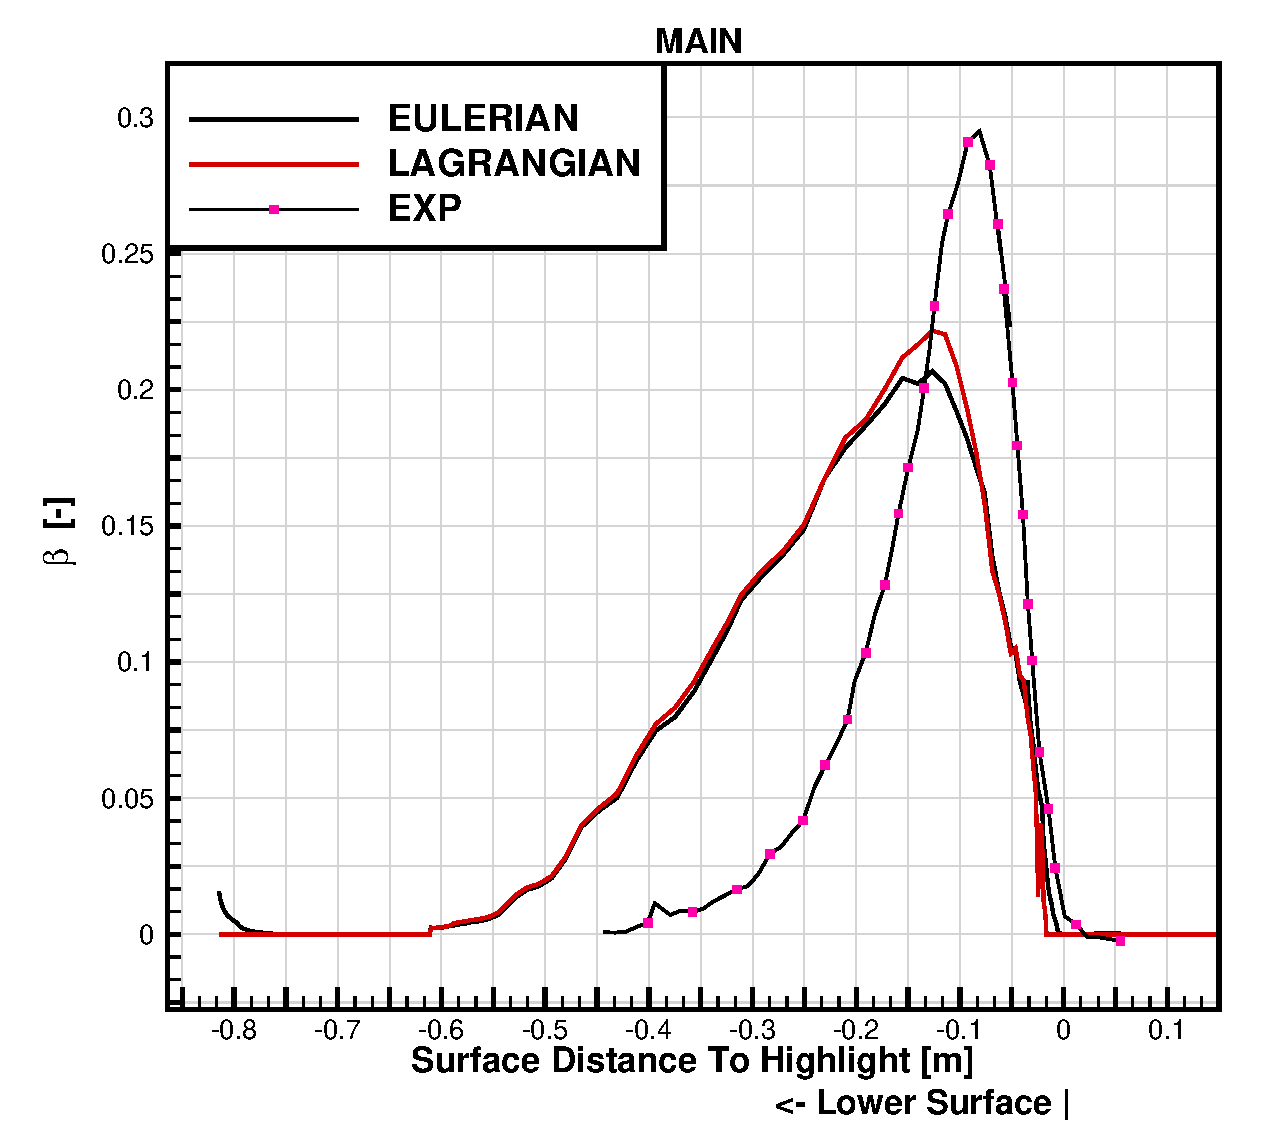
\includegraphics[width=0.325\textwidth]{FIGURES/LAGRANGIAN_ARTICLE/CASE_122_MAIN_DISTRIBUTION.eps}
\label{fig:MDA_MAIN_DISTRIBUTION}%
}
%\hspace*{-1cm}
\subfloat[\centering Impingement results on the Flap.]{%
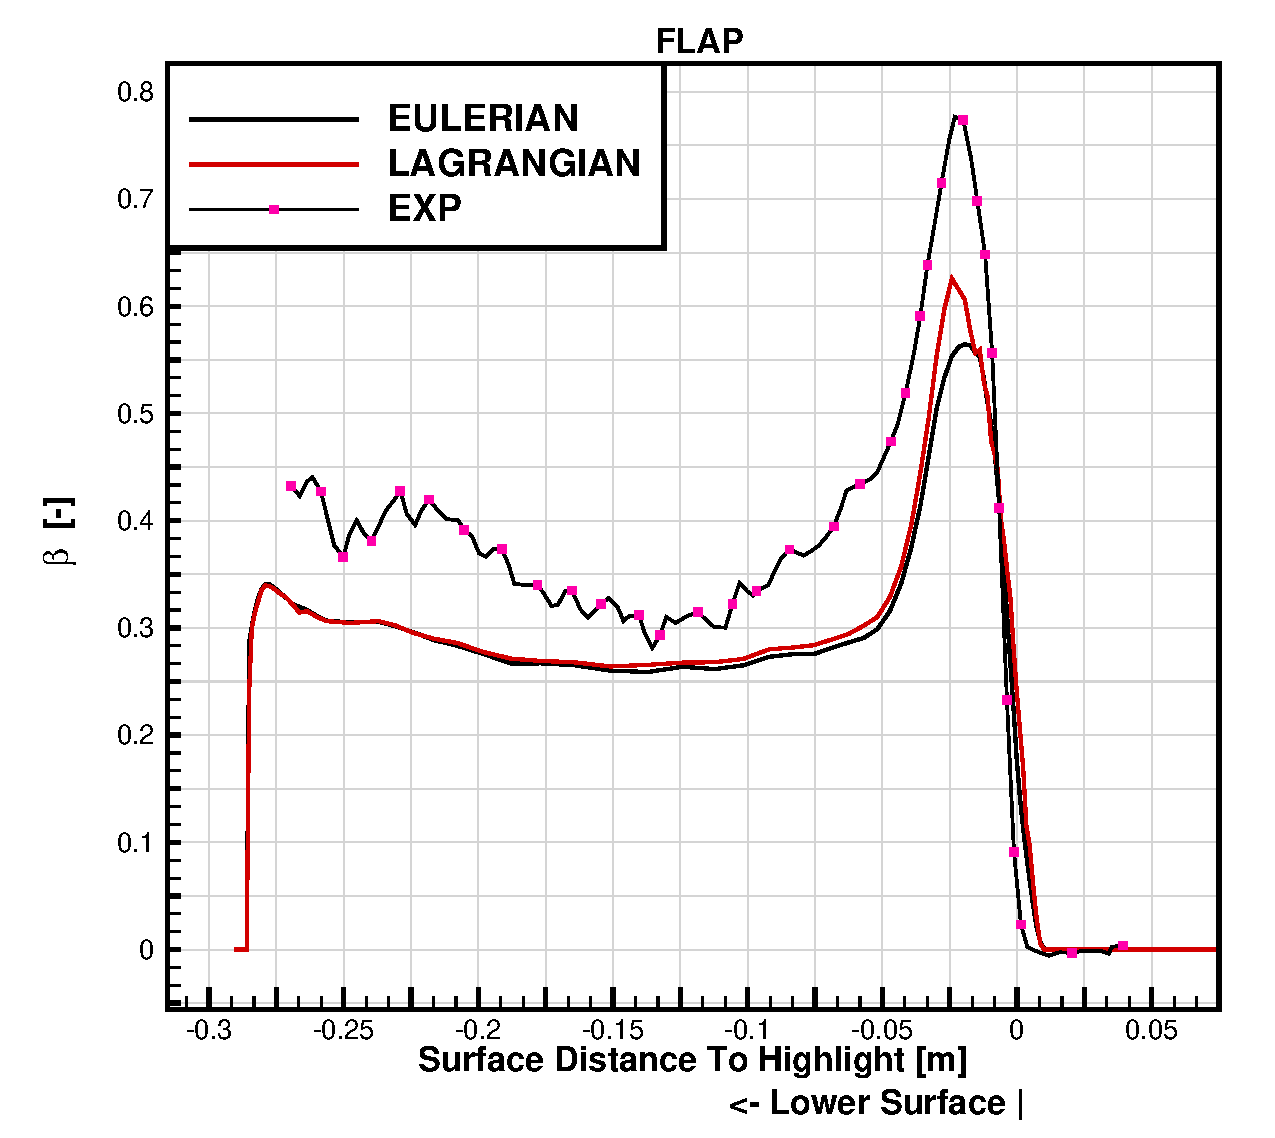
\includegraphics[width=0.325\textwidth]{FIGURES/LAGRANGIAN_ARTICLE/CASE_122_FLAP_DISTRIBUTION.eps}
\label{fig:MDA_FLAP_DISTRIBUTION}%
}

\hspace*{-1cm}
\subfloat[SLD results on the Slat.]{%
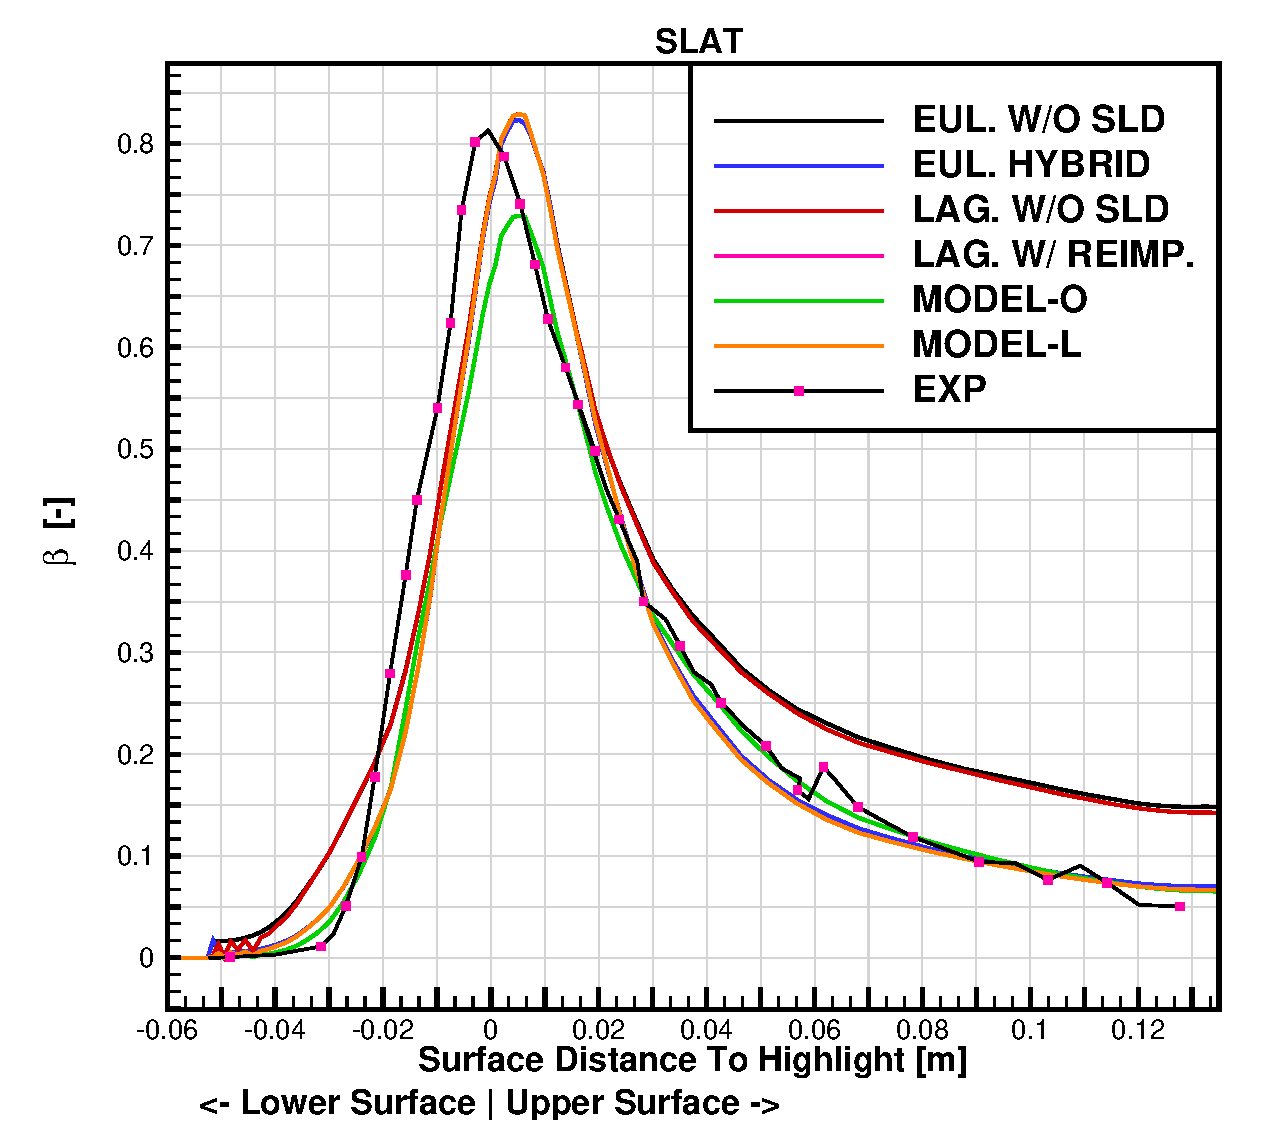
\includegraphics[width=0.325\textwidth]{FIGURES/LAGRANGIAN_ARTICLE/CASE_122_SLAT_SLD.eps} \quad
\label{fig:MDA_SLAT_SLD}%
}%
%\hspace*{-1cm}
\subfloat[SLD results on the Main.]{%
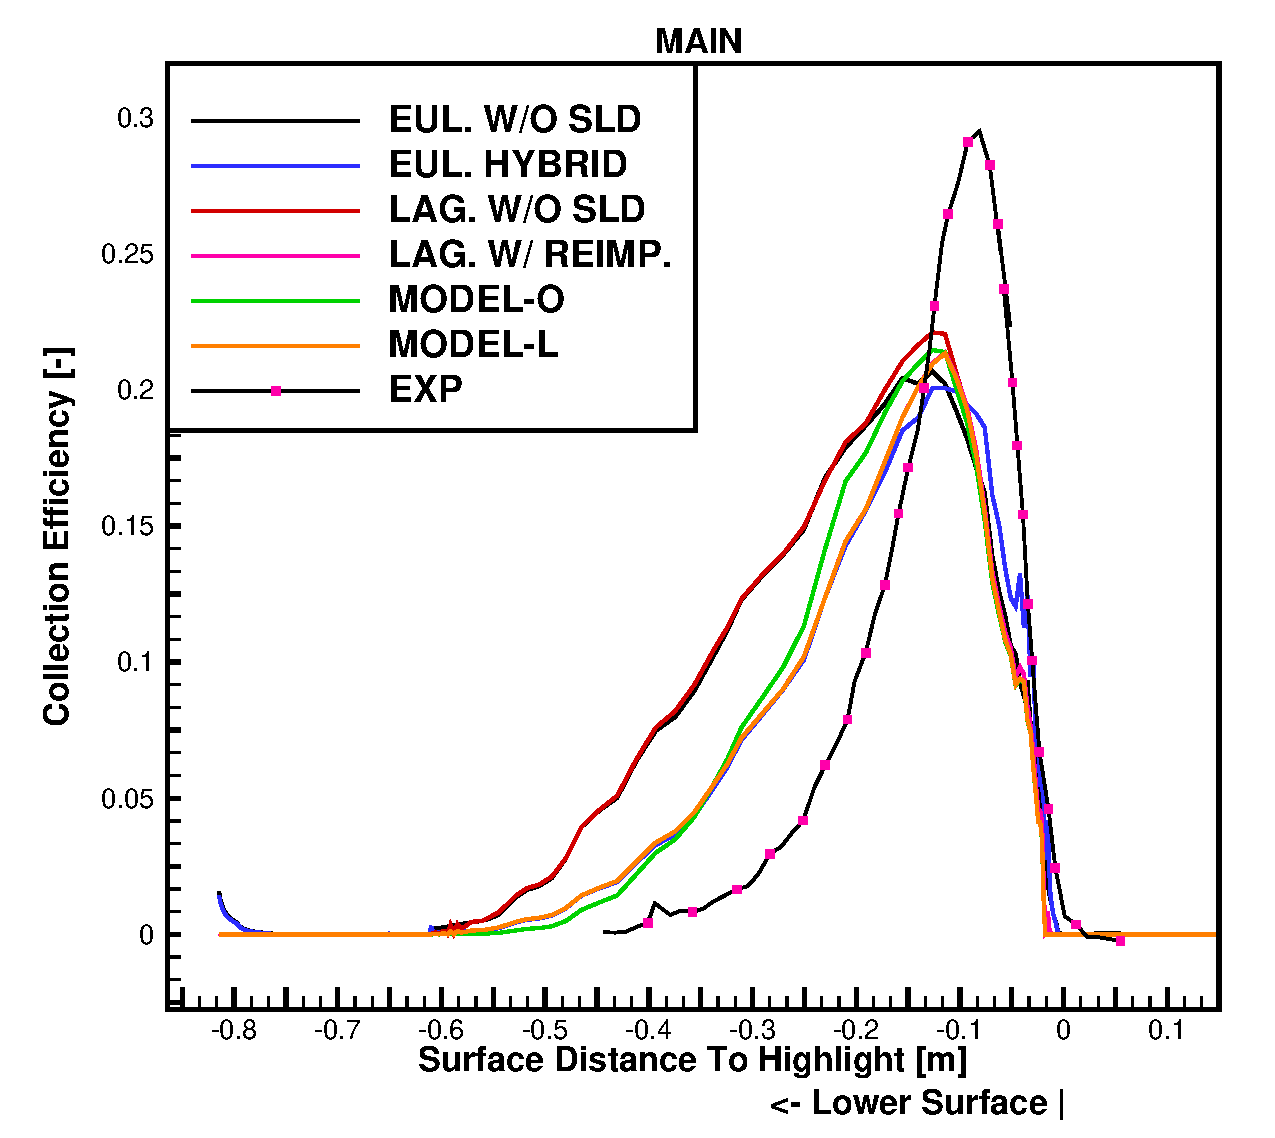
\includegraphics[width=0.325\textwidth]{FIGURES/LAGRANGIAN_ARTICLE/CASE_122_SLAT_MAIN.eps}
\label{fig:MDA_MAIN_SLD}%
}
%\hspace*{-1cm}
\subfloat[SLD results on the Flap.]{%
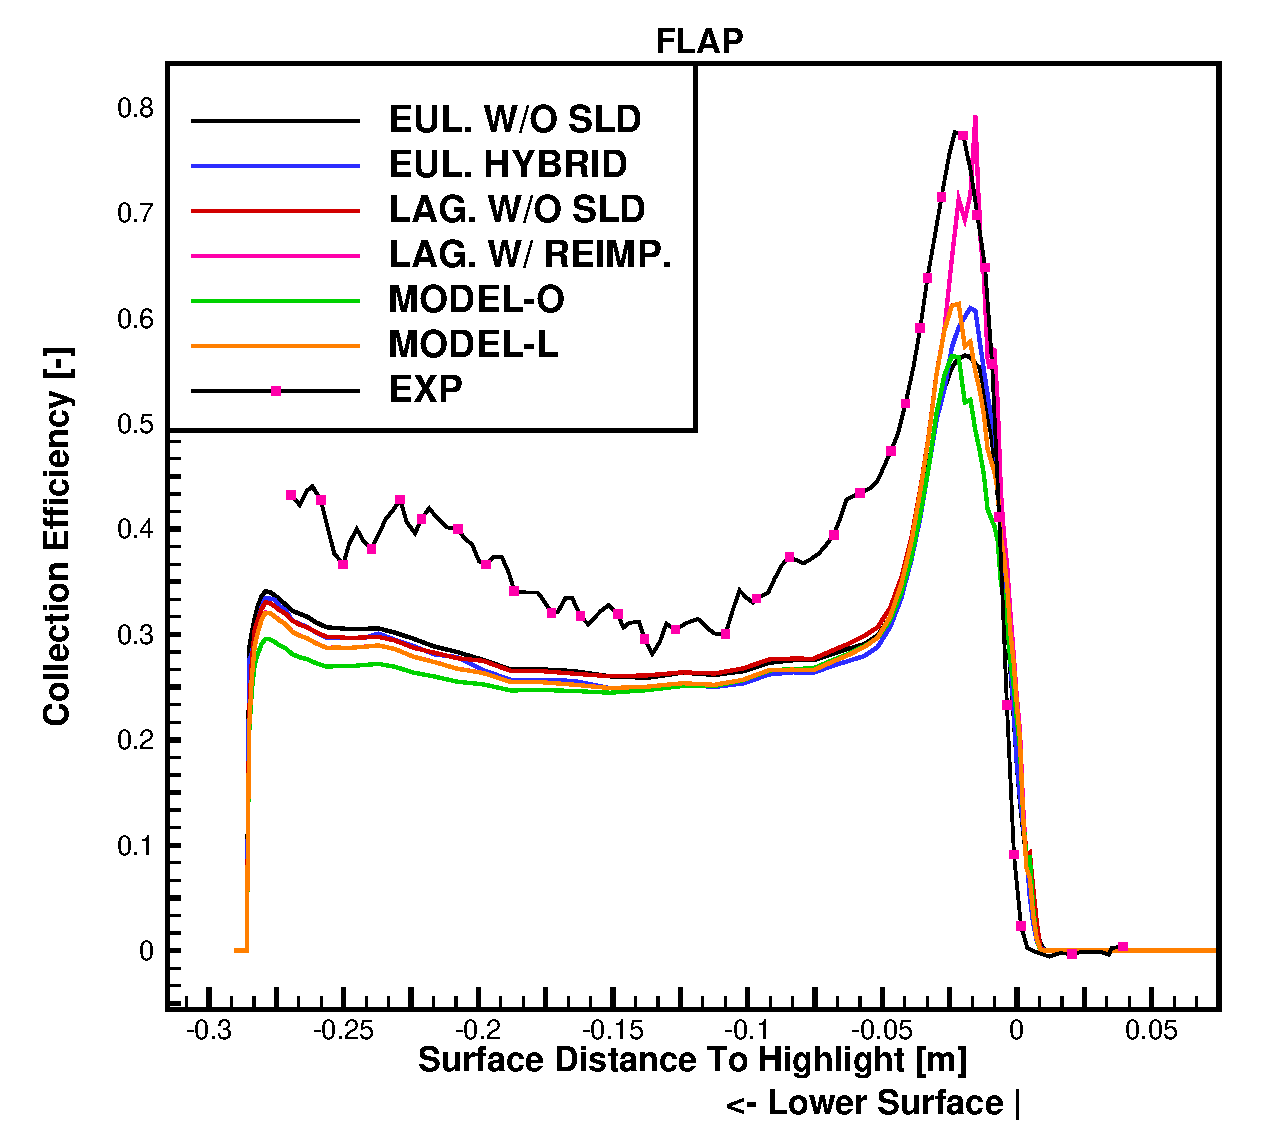
\includegraphics[width=0.325\textwidth]{FIGURES/LAGRANGIAN_ARTICLE/CASE_122_SLAT_FLAP.eps}
\label{fig:MDA_FLAP_SLD}%
}
\caption{ Results of CASE IPW1 - 122.}
\label{fig:MDA}
\end{figure}


\subsection{Case IPW2 - 1.3 : Hybrid CRM (With Gap)}
This case poses significant challenges due to the gap between the top of the airfoil and the wind tunnel wall (Fig. \ref{fig:CASE_1p3_GAP}). In one of the available meshes from the workshop, the gap was included and explicitly meshed, whereas in the other, the gap was ignored. The presence of this gap presents difficulties at both the flow solver and droplet solver levels, primarily due to the recirculation zone formed in this region, similar to the previous case but here investigated for a 3D geometry. While ice accretion diminishes this gap over time, as demonstrated by experimental ice shapes, the initial layer of ice remains influenced by its presence. Moreover, this test case serves as an excellent opportunity to evaluate the capabilities of the Lagrangian solver under such conditions. The results for this test case are illustrated in Fig. \ref{fig:CASE_1p3}. The initial comparisons show strong agreement between Eulerian and Lagrangian results accross all the cuts, with discrepancies appearing near the impingement limits. This trend is further highlighted in the contour plot of the collection efficiency shown in Fig. \ref{fig:CASE_1p3_Contour}. The latter showcase the relative difference between Lagrangian and Eulerian results with respect to collection efficiency calculated as follows:

\begin{equation}
\beta_{\text{RelativeDifference}} = \frac{\vert \beta_{\text{Lagrangian}} - \beta_{\text{Eulerian}} \vert}{\beta_{\text{Lagrangian}}}
\end{equation}

\noindent Values below $10\%$ are omitted from the plot for clarity (colored in Grey). The observed differences are most pronounced near the impingement region, a consistent trend across all test cases. Additionally, the differences are positive (when not taking the absolute value), indicating that the Lagrangian solver predicts slightly larger impingement limits compared to the Eulerian solver. This observation should be further investigated in future work when comparing ice shapes derived from both models. Other discrepancies are also noticeable near the gap where the Eulerian solver usually have difficulty to predict impingement data.

\begin{figure}[h!]
\hspace*{-1cm}
\subfloat[Case IPW2 1.3 Geometry.]{%
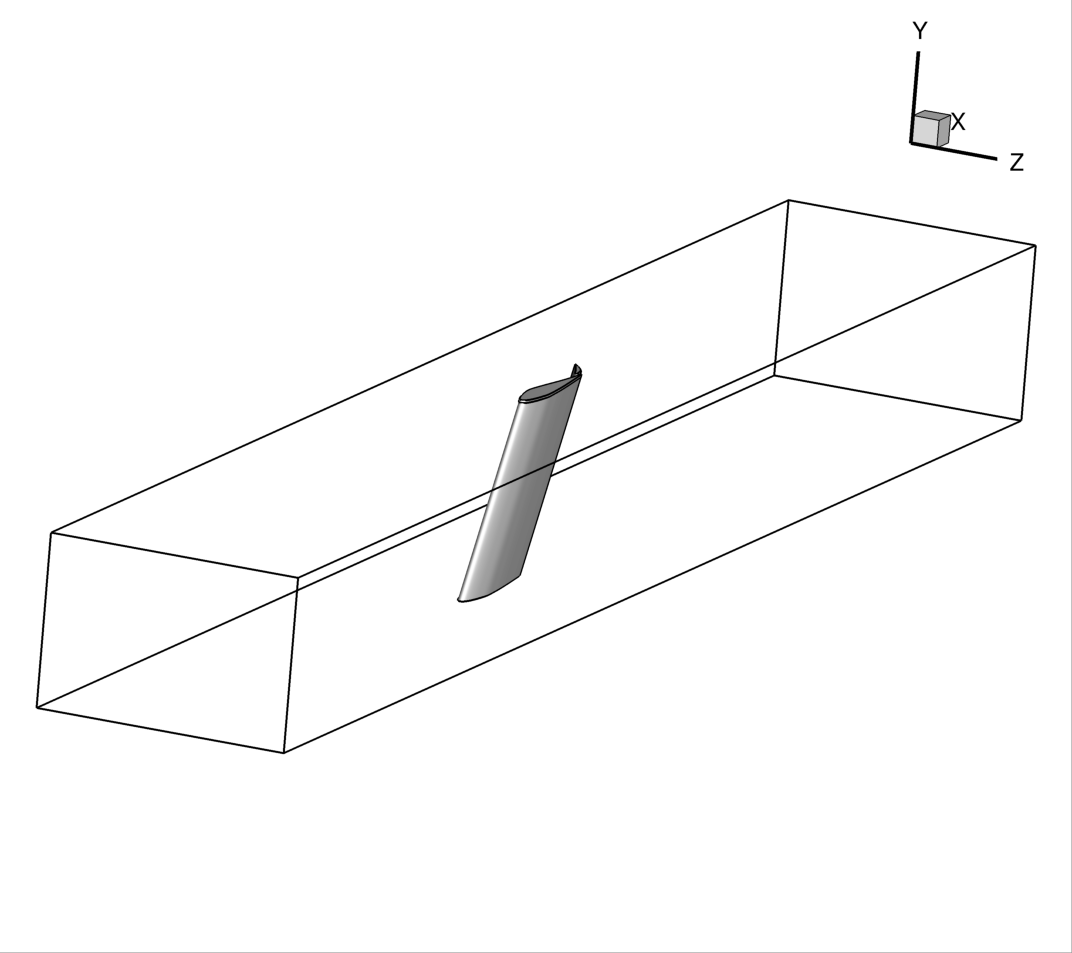
\includegraphics[width=0.49\textwidth]{FIGURES/LAGRANGIAN_ARTICLE/GEO.png}
\label{fig:CASE_1p3_GEO}%
}
%\hspace*{-1cm}
\subfloat[Case IPW2 1.3 Gap region with the wind tunnel.]{%
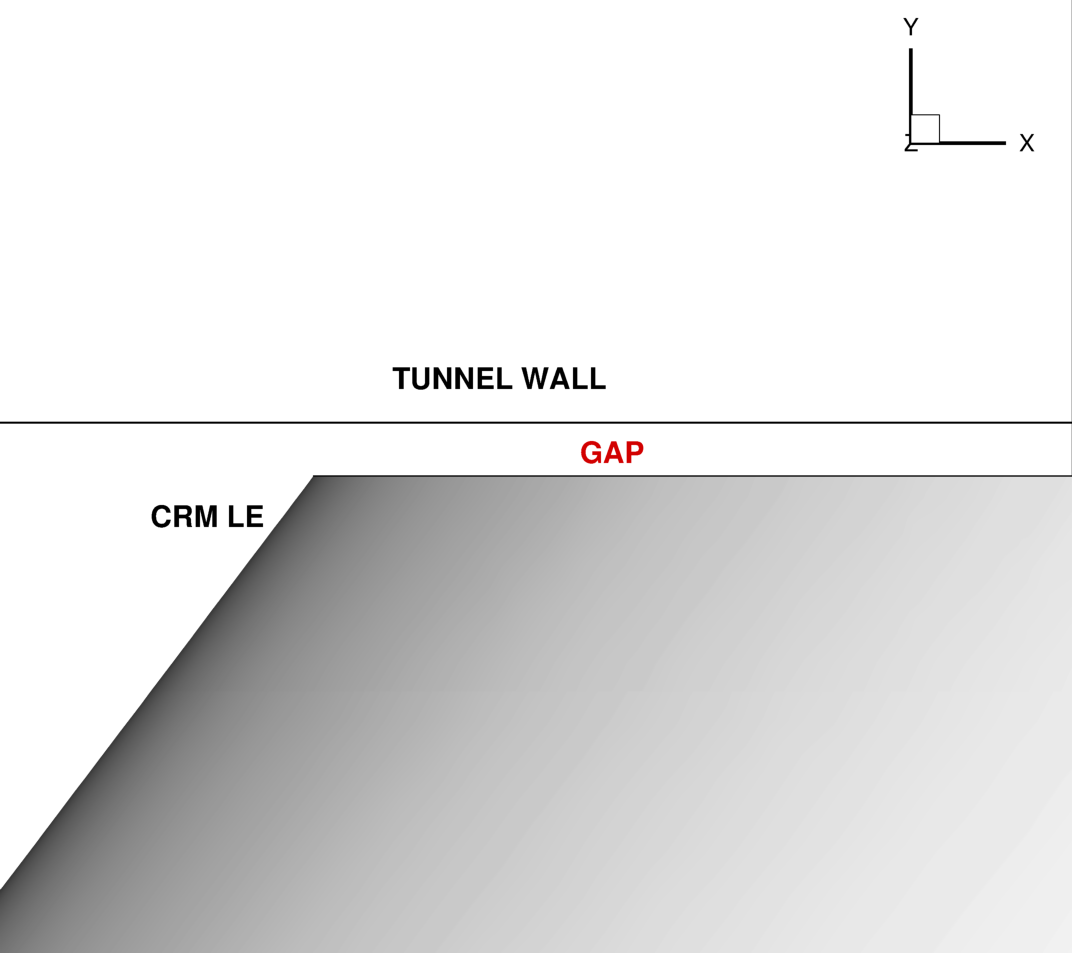
\includegraphics[width=0.49\textwidth]{FIGURES/LAGRANGIAN_ARTICLE/GAP.png}
\label{fig:CASE_1p3_GAP}%
}
\caption{ Description of Case IPW2 1.3}
\label{fig:CASE_1p3_Description}
\end{figure}

\begin{figure}[ht]
\vspace{-1cm}
\centering
\hspace*{-0.5cm}
\subfloat[Impingement Results on Station 1 : 18 inches.]{%
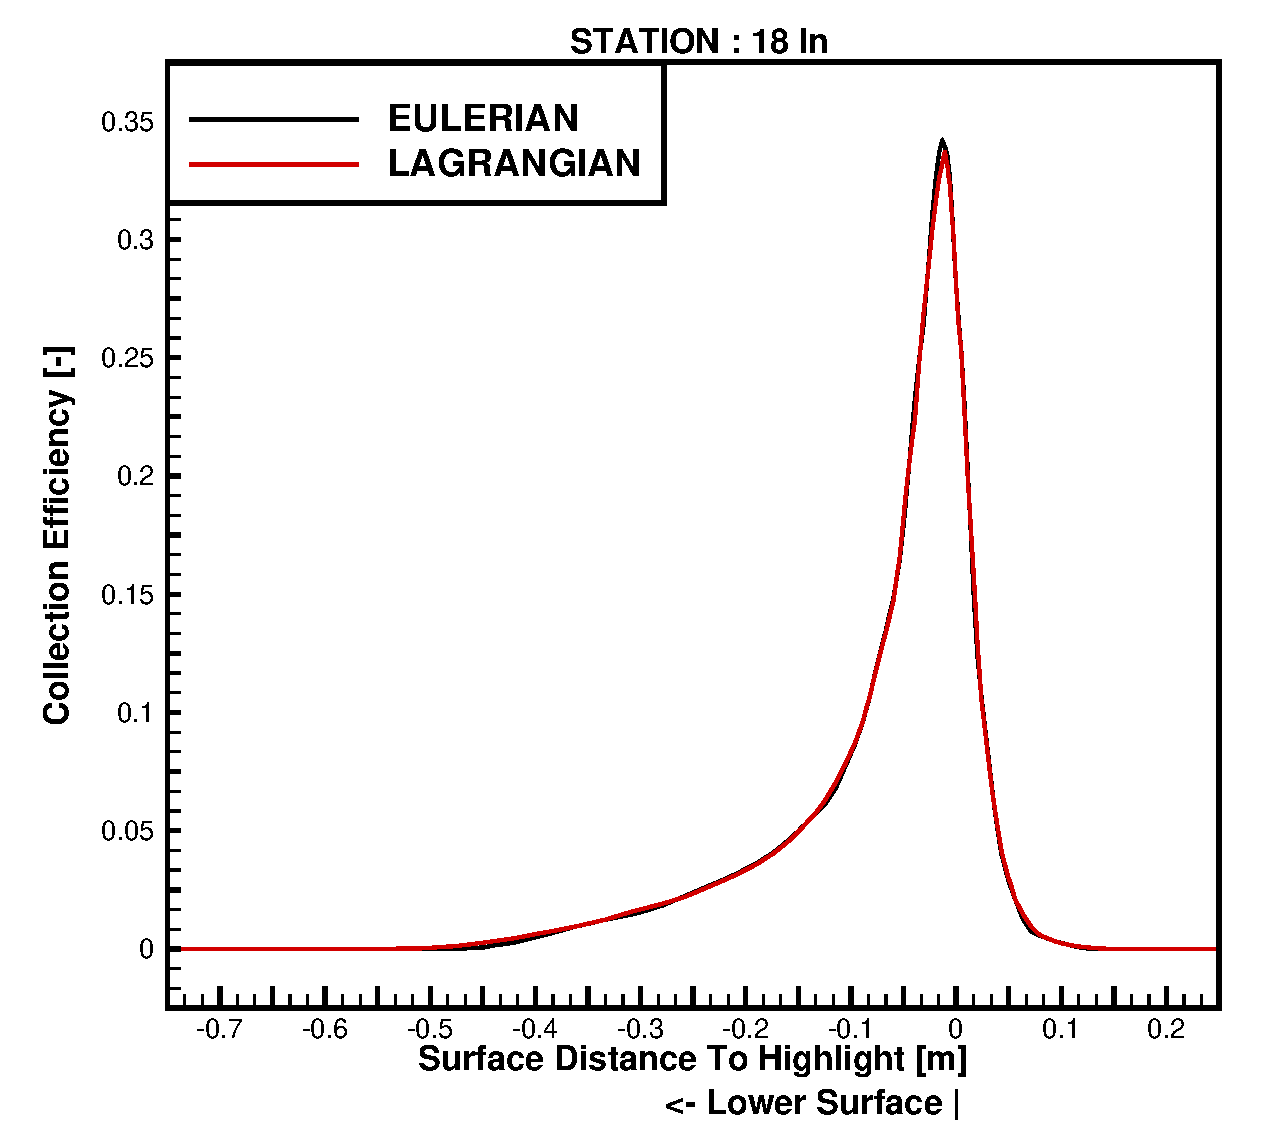
\includegraphics[trim={0cm 0.05cm 0.05cm 0cm}, clip, width=0.5\textwidth]{FIGURES/LAGRANGIAN_ARTICLE/CASE_1p3_18IN.eps}   
\label{fig:CASE_1p3_18}}
\subfloat[Impingement Results on Station 2 : 36 inches.]{%
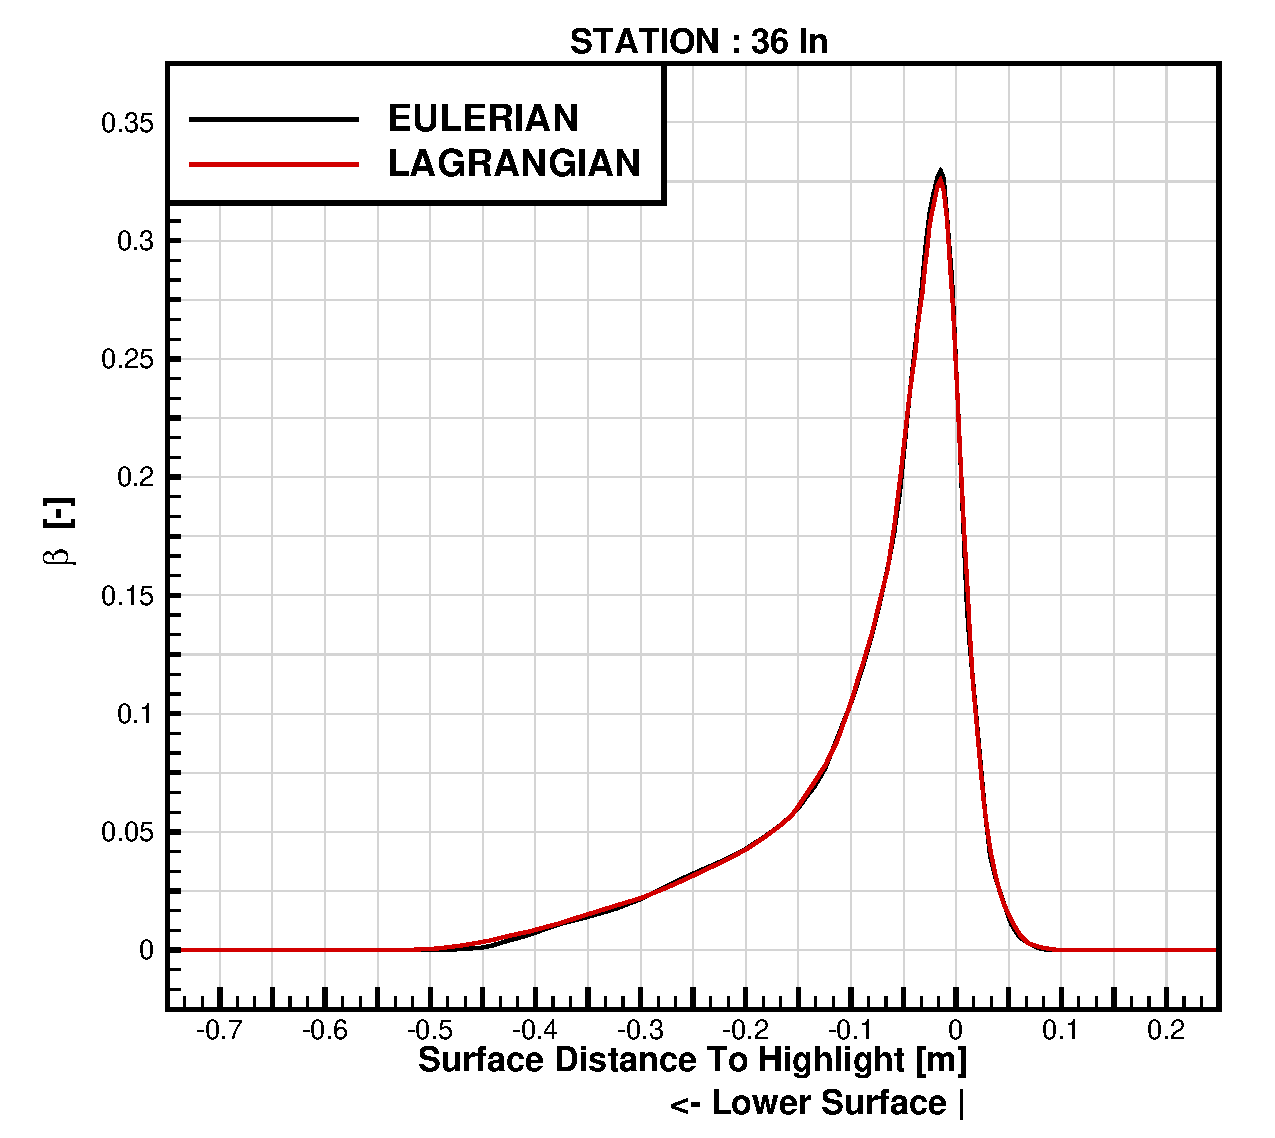
\includegraphics[trim={0cm 0.05cm 0.05cm 0cm}, clip, width=0.5\textwidth]{FIGURES/LAGRANGIAN_ARTICLE/CASE_1p3_36IN.eps}
\label{fig:CASE_1p3_36}%
}

\hspace*{-1cm}
\centering
\subfloat[Impingement Results on Station 3 : 54 inches.]{%
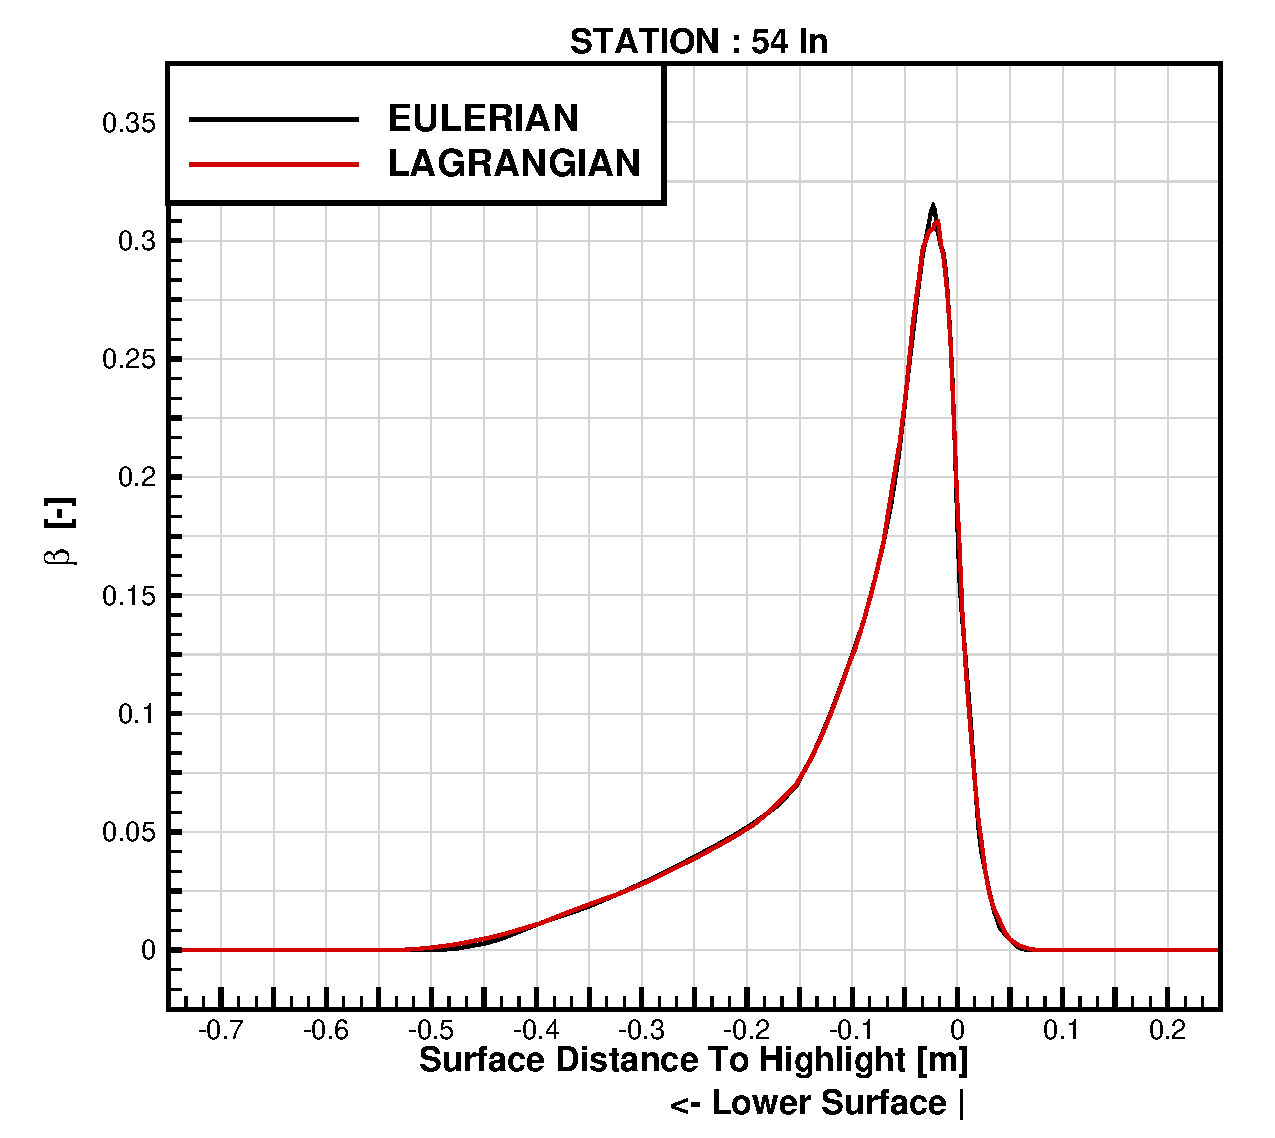
\includegraphics[trim={0cm 0.05cm 0.05cm 0cm}, clip, width=0.49\textwidth]{FIGURES/LAGRANGIAN_ARTICLE/CASE_1p3_54IN.eps}
\label{fig:CASE_1p3_54}%
}
\subfloat[Relative Difference Between Eulerian and Lagrangian Solutions in Terms of Collection Efficiency.]{%
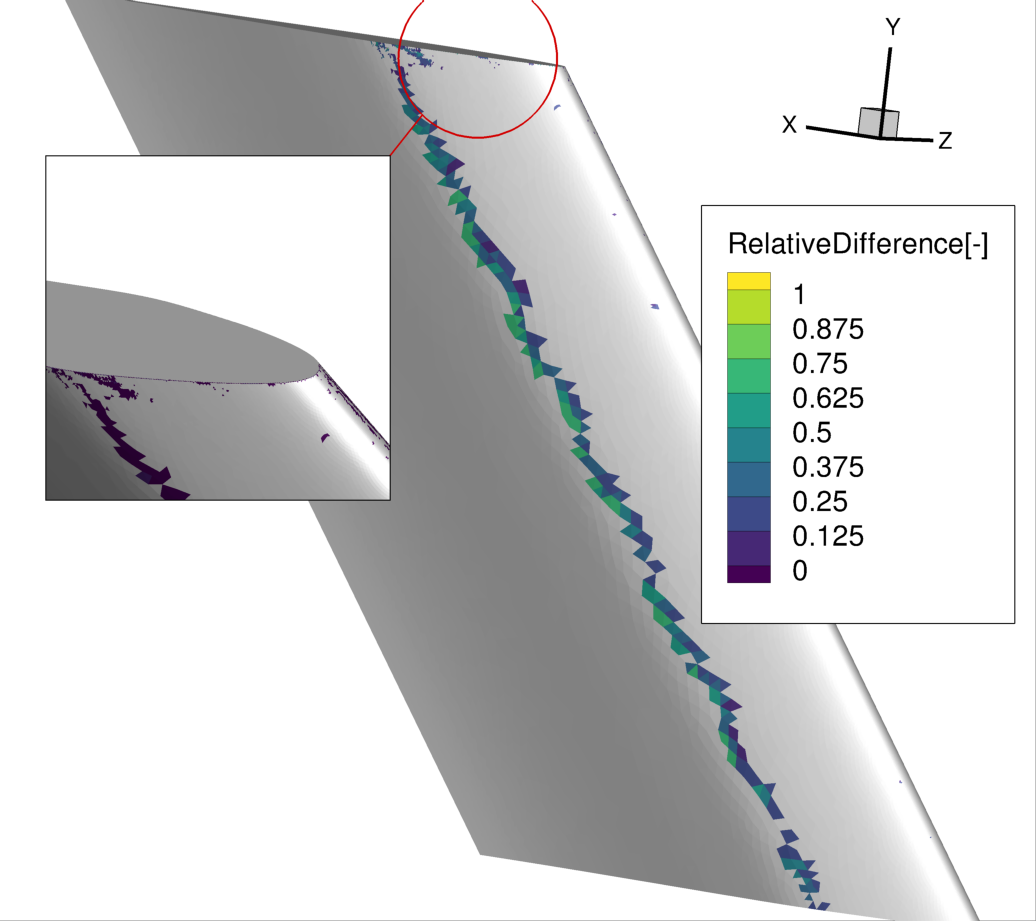
\includegraphics[trim={0cm 0.05cm 0.05cm 0cm}, clip, width=0.49\textwidth]{FIGURES/LAGRANGIAN_ARTICLE/difference.png}
\label{fig:CASE_1p3_Contour}%
}%
\caption{Results for CASE IPW2 - 1.3.}
\label{fig:CASE_1p3}
\end{figure}

\subsection{Case HLPW5 - 2.1 : CRM Wing-Body}
The final case, using the Common Research Model (CRM), assesses the solver’s performance and accuracy on a larger, more complex configuration representative of an industrial aircraft. The impingement results for Case HLPW5 - 2.1 are presented in Fig. \ref{fig:2p1}. These results were extracted using cuts along the wing span and fuselage. The placement of these cuts is detailed in Fig. \ref{fig:cuts}. 

\begin{figure}[htp]
\vspace{-1cm} % Adjust the value as needed
\hspace*{-1cm}
\subfloat[\centering  Impingement results on the Fuselage.]{%
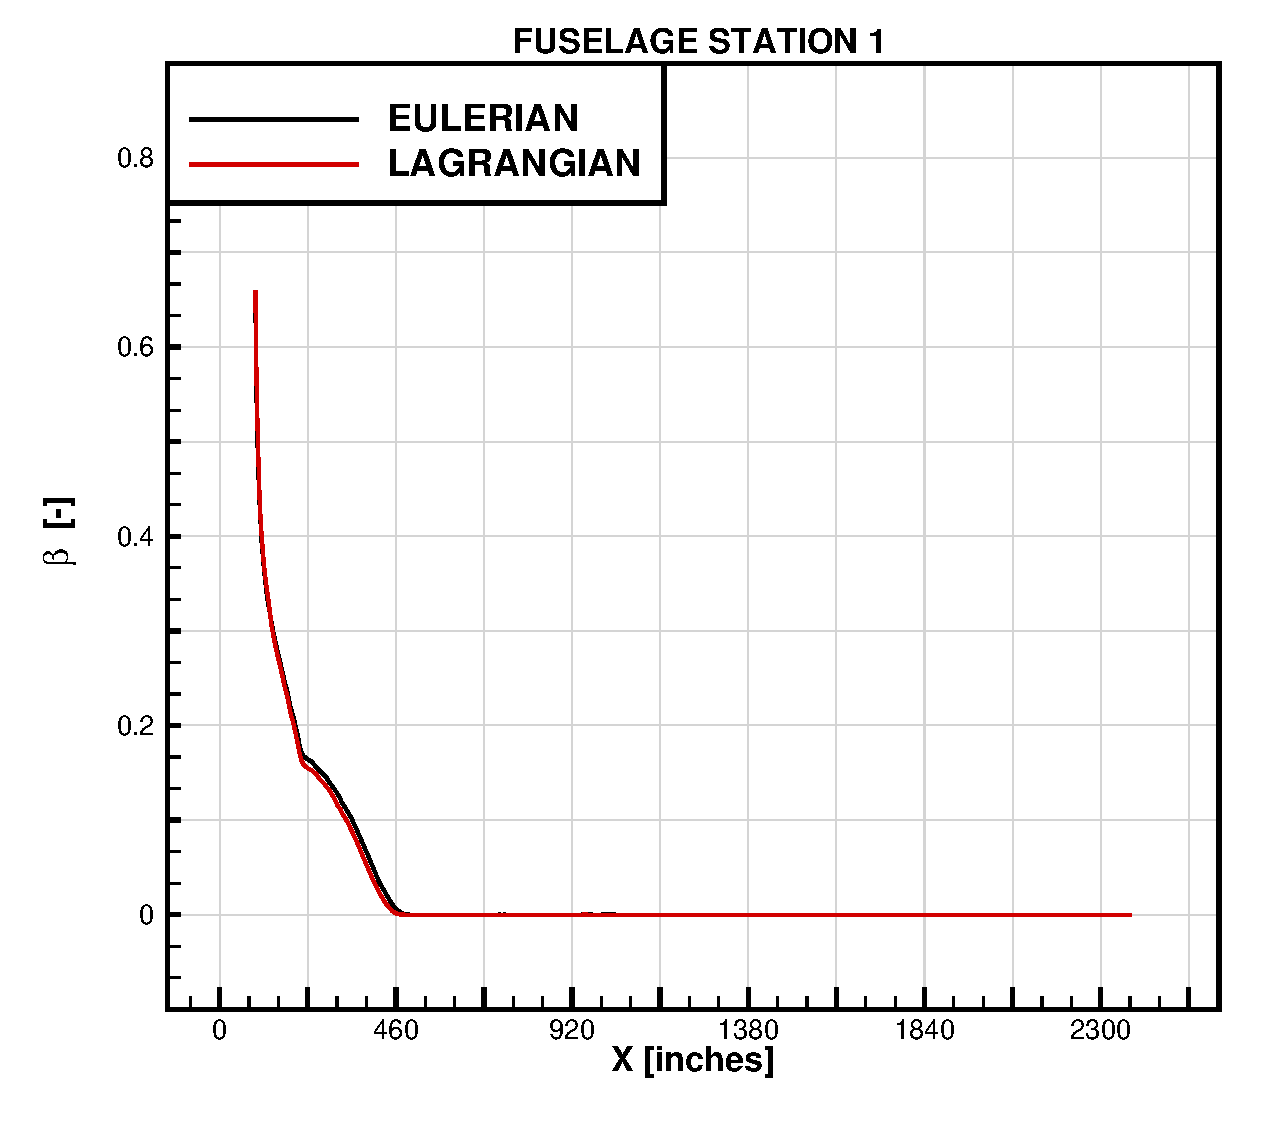
\includegraphics[width=0.325\textwidth]{FIGURES/LAGRANGIAN_ARTICLE/CASE_2p1_FUSELAGE_DISTRIBUTION.eps} \quad
\label{fig:CRM_FUSELAGE}%
}%
\subfloat[\centering Impingement results on the Wing-1.]{%
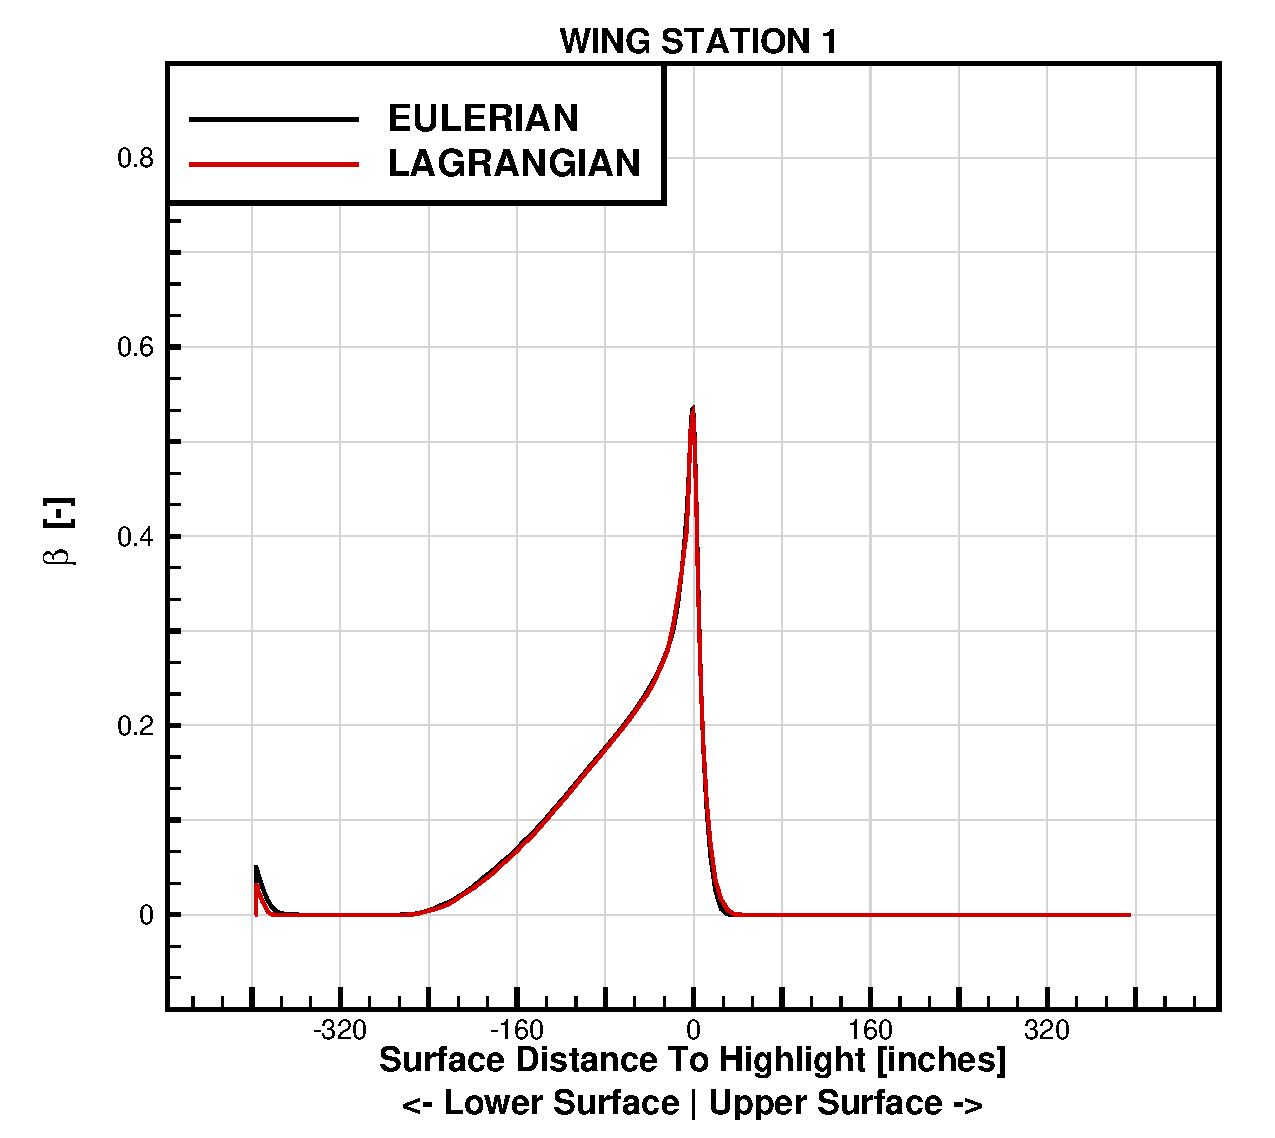
\includegraphics[width=0.325\textwidth]{FIGURES/LAGRANGIAN_ARTICLE/CASE_2p1_WING_1_DISTRIBUTION.eps}
\label{fig:CRM_WING_1}%
}
\subfloat[\centering Impingement results on the Wing-2.]{%
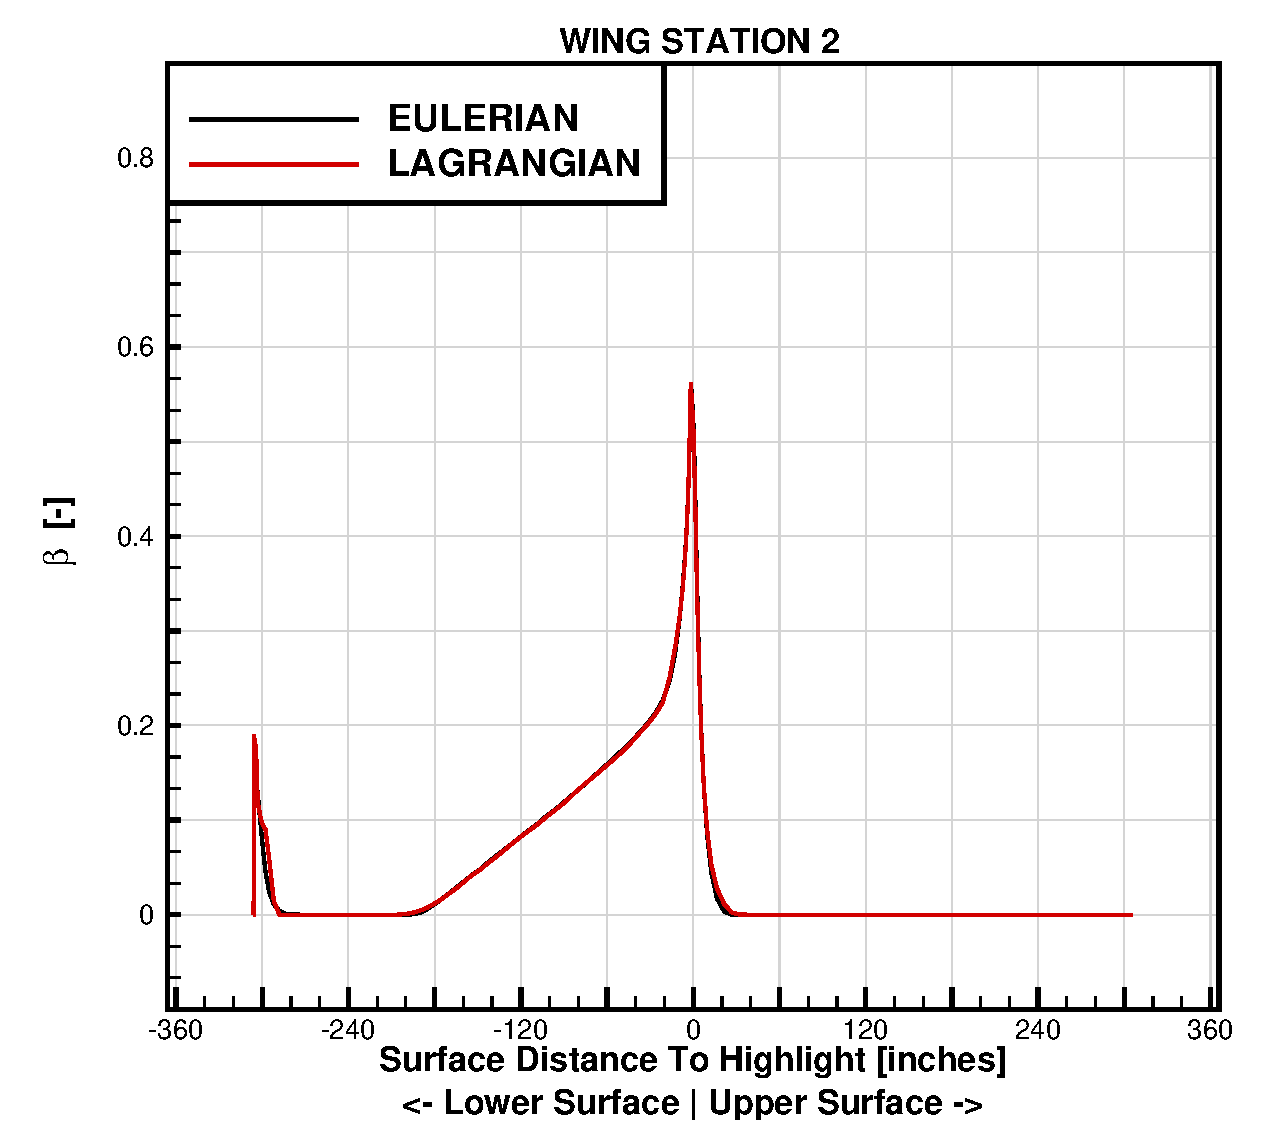
\includegraphics[width=0.325\textwidth]{FIGURES/LAGRANGIAN_ARTICLE/CASE_2p1_WING_2_DISTRIBUTION.eps}
\label{fig:CRM_WING_2}%
}

\hspace*{-1cm}
\subfloat[\centering Impingement results on the Wing-3.]{%
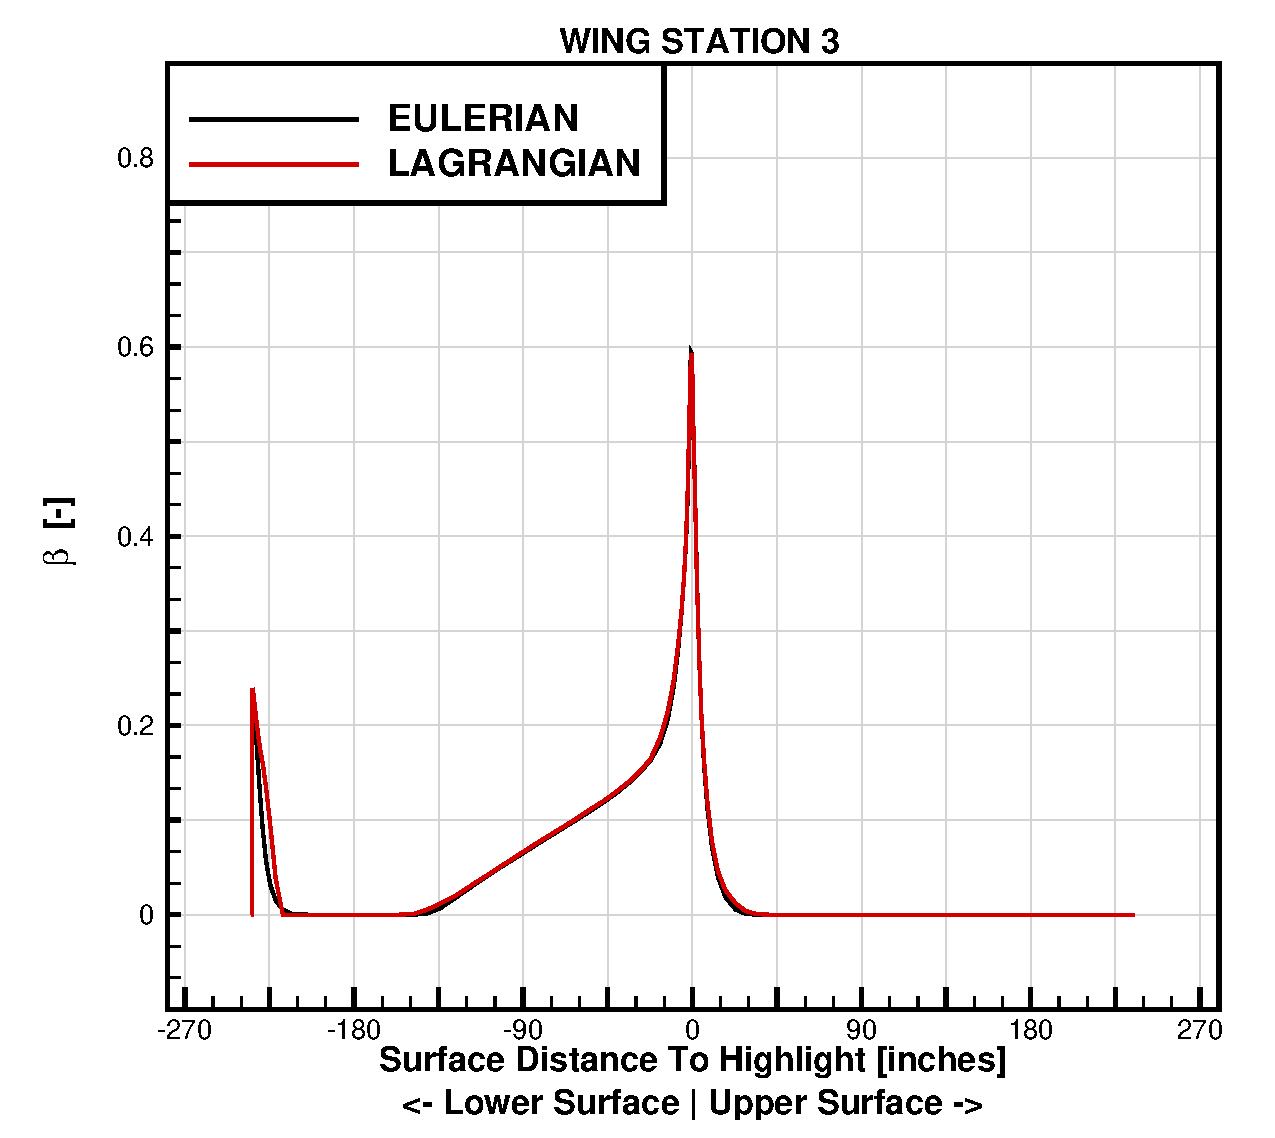
\includegraphics[width=0.325\textwidth]{FIGURES/LAGRANGIAN_ARTICLE/CASE_2p1_WING_3_DISTRIBUTION.eps} \quad
\label{fig:CRM_WING_3}%
}%
\subfloat[\centering Impingement results on the Wing-4.]{%
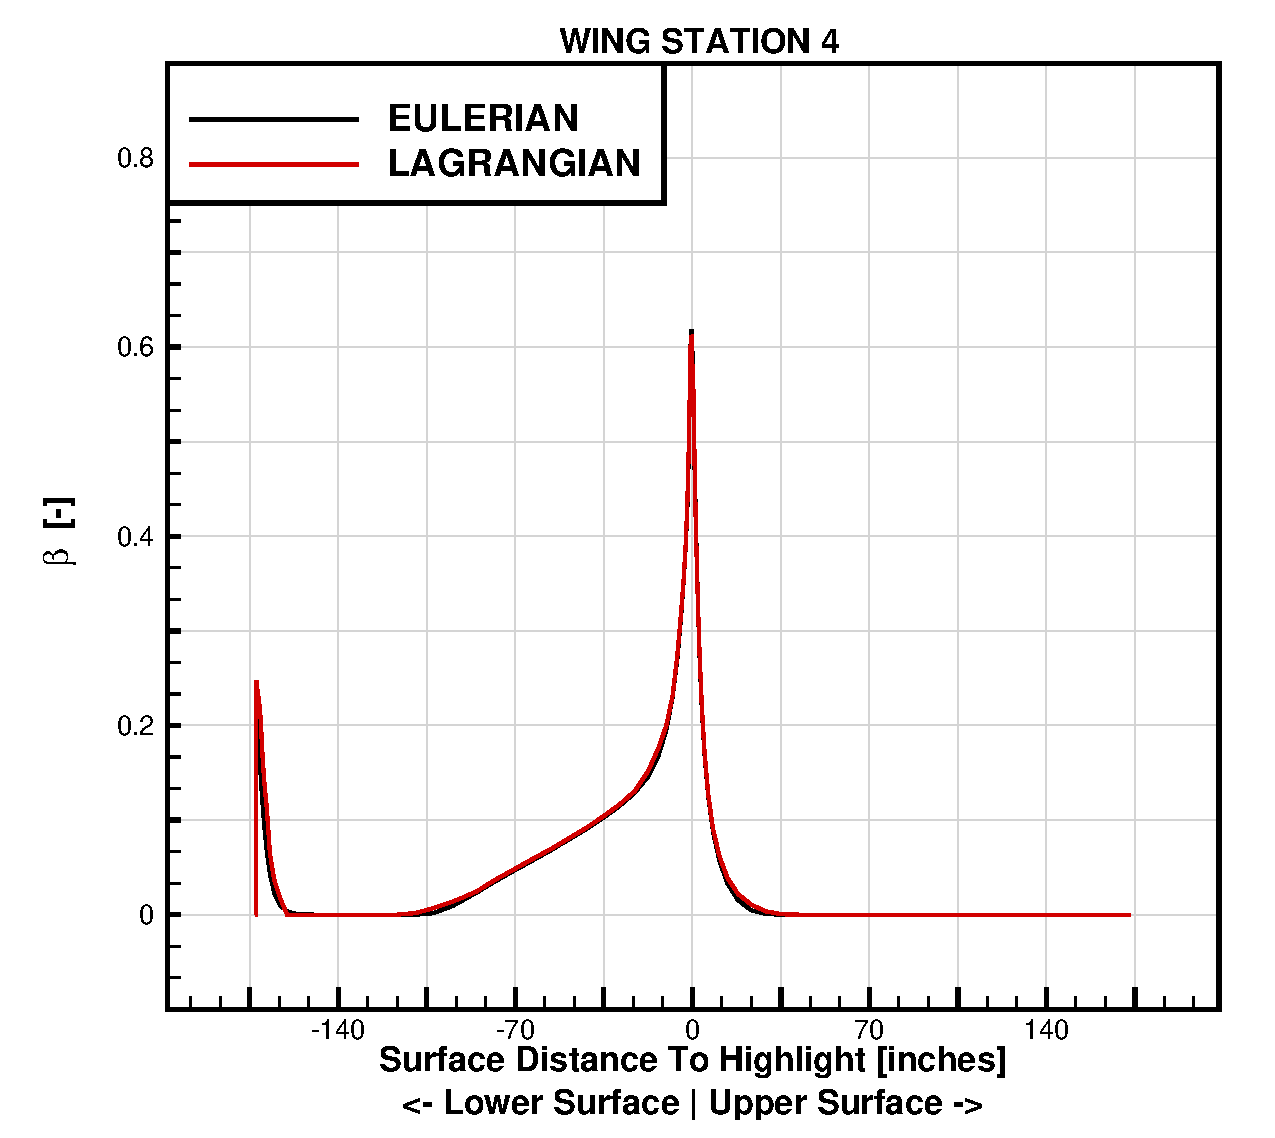
\includegraphics[width=0.325\textwidth]{FIGURES/LAGRANGIAN_ARTICLE/CASE_2p1_WING_4_DISTRIBUTION.eps}
\label{fig:CRM_WING_4}%
}
\subfloat[\centering Impingement results on the Wing-5.]{%
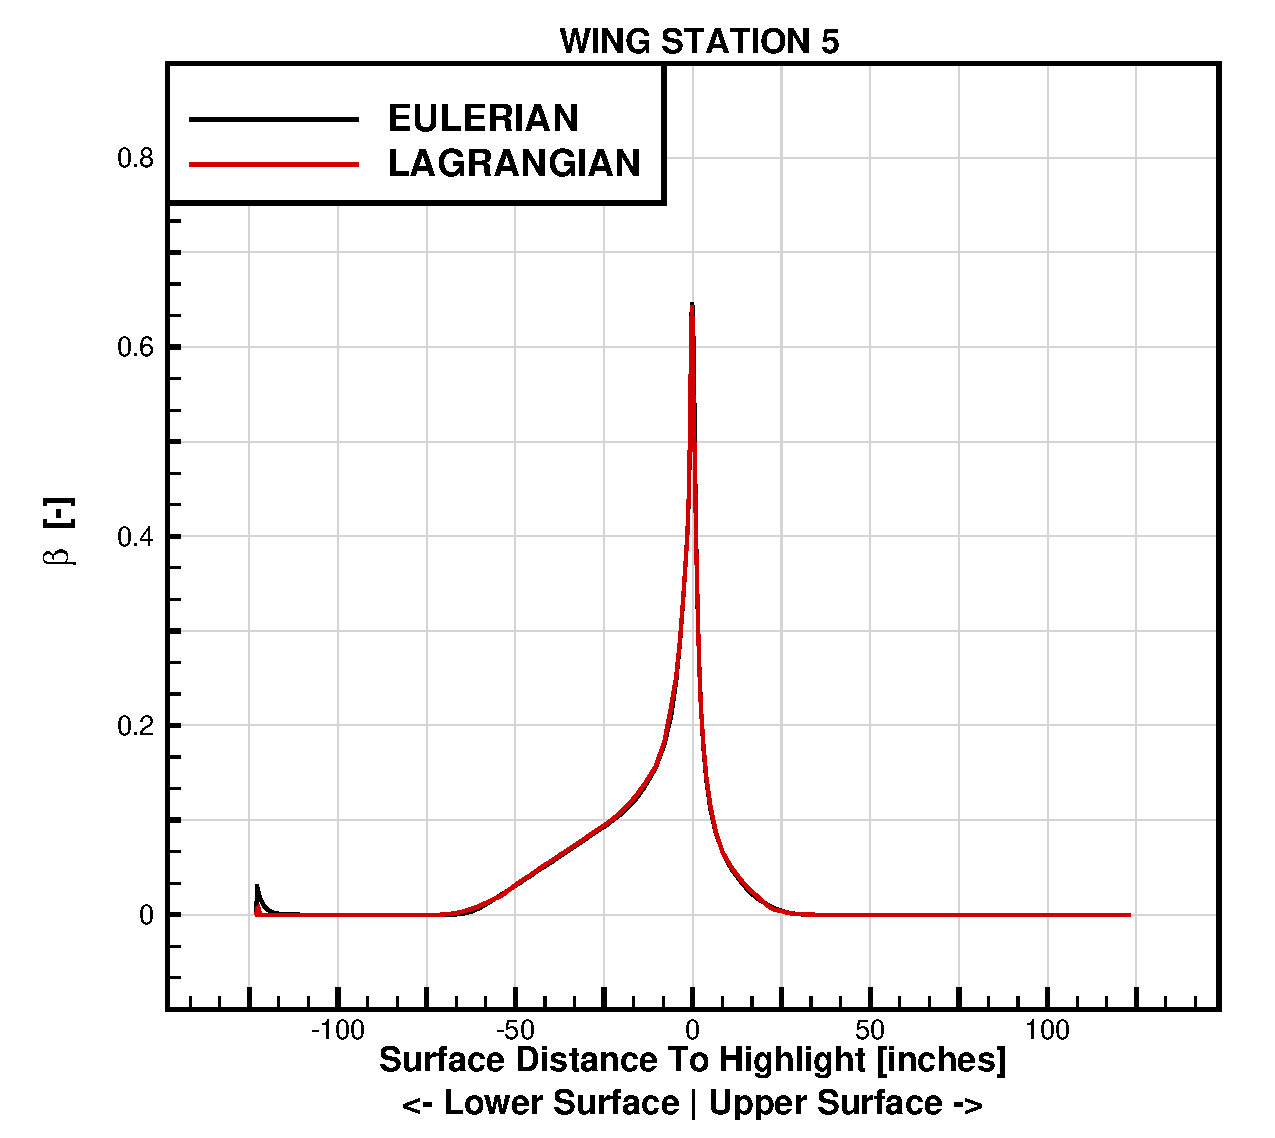
\includegraphics[width=0.325\textwidth]{FIGURES/LAGRANGIAN_ARTICLE/CASE_2p1_WING_5_DISTRIBUTION.eps}
\label{fig:CRM_WING_5}%
}

\hspace*{-1cm}
\subfloat[\centering SLD results on the Fuselage.]{%
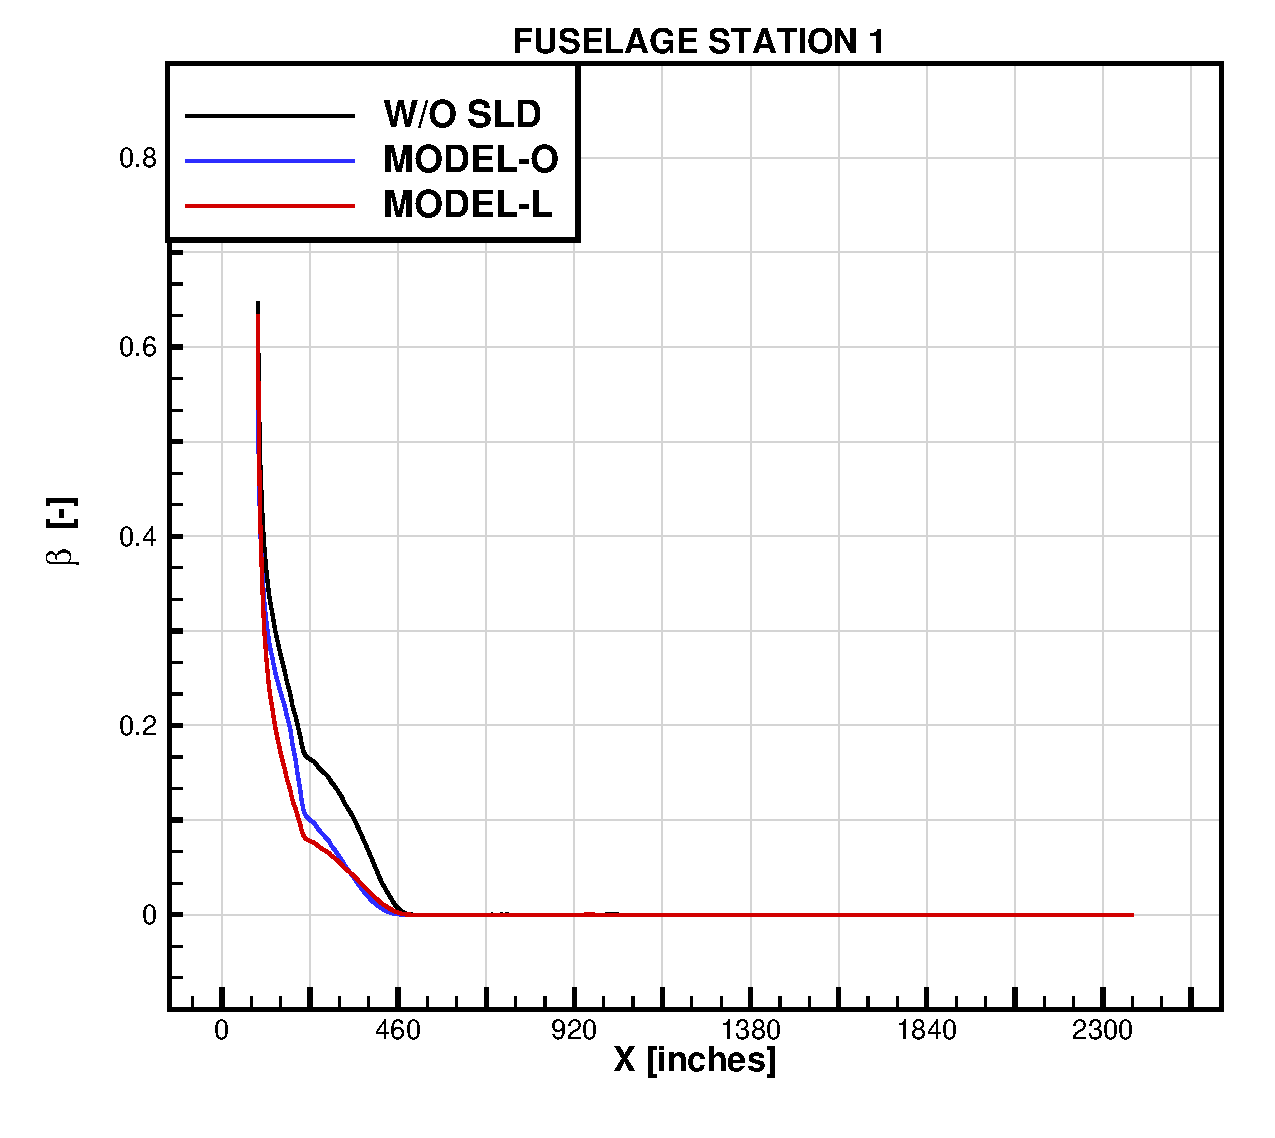
\includegraphics[width=0.325\textwidth]{FIGURES/LAGRANGIAN_ARTICLE/CASE_2p1_FUSELAGE_SLD.eps} \quad
\label{fig:CRM_FUSELAGE_SLD}%   
}%
\subfloat[\centering SLD results on the Wing-1.]{%
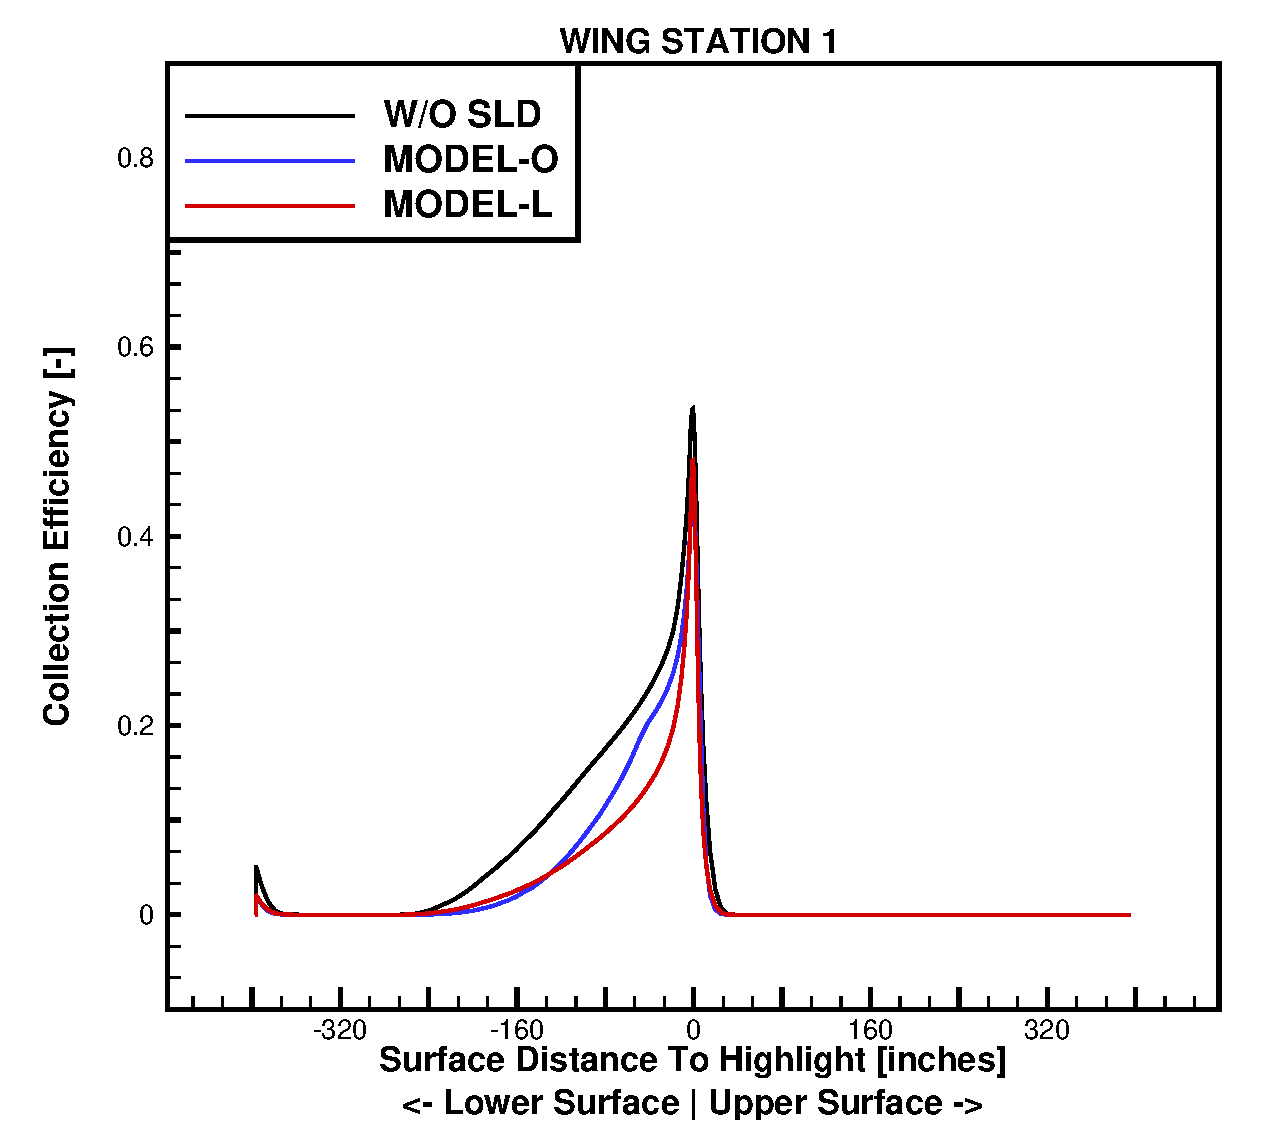
\includegraphics[width=0.325\textwidth]{FIGURES/LAGRANGIAN_ARTICLE/CASE_2p1_WING_1_SLD.eps}
\label{fig:CRM_WING_1_SLD}%
}
\subfloat[\centering SLD results on the Wing-2.]{%
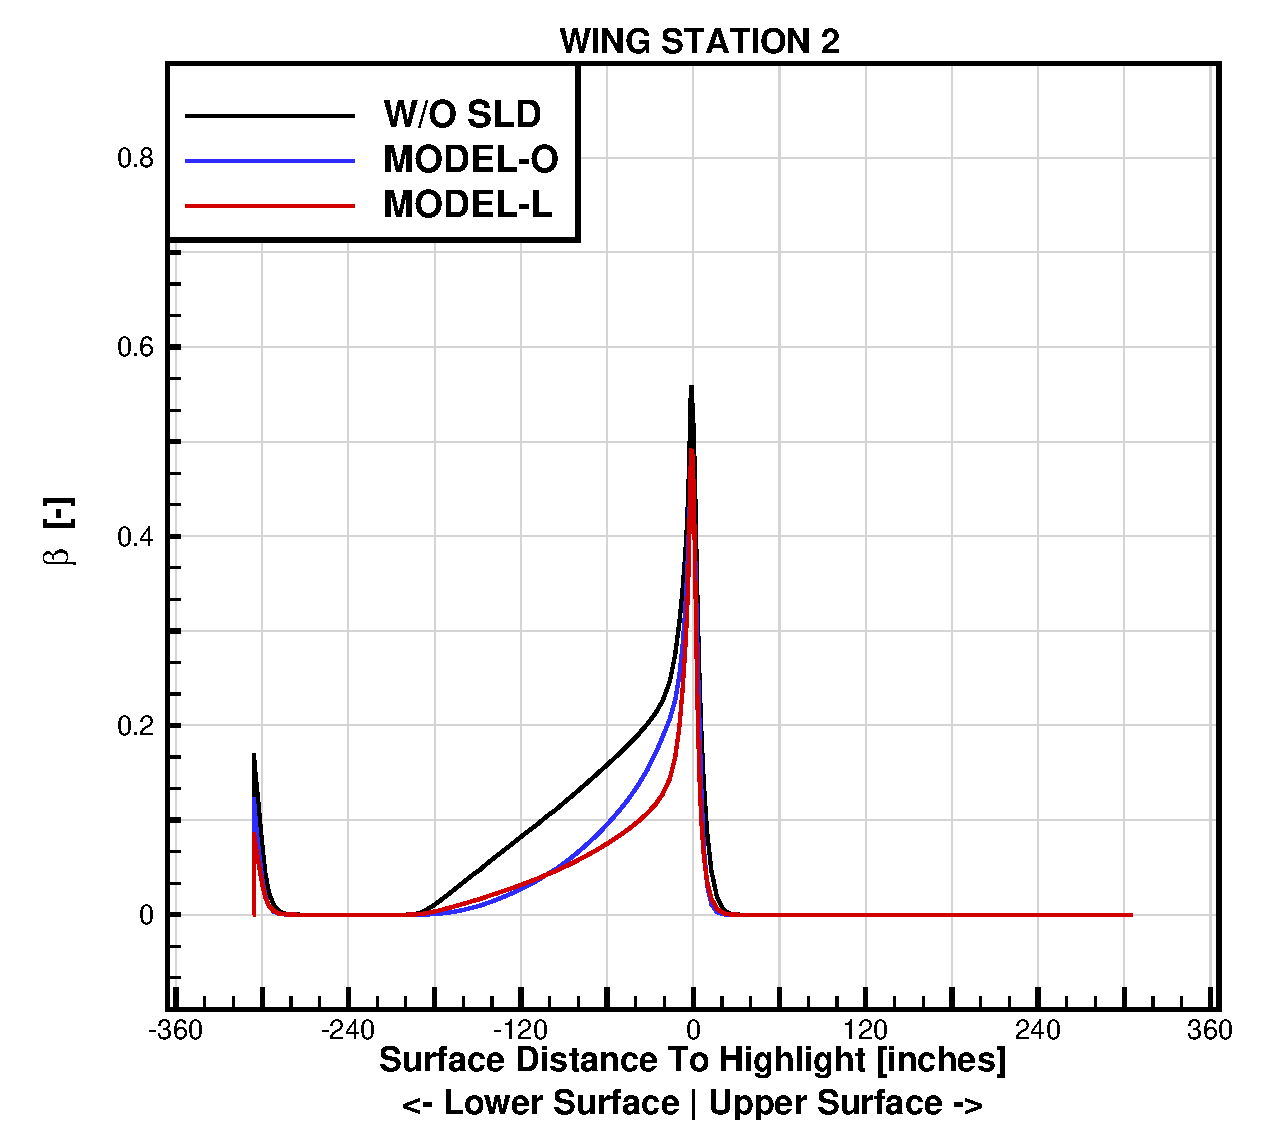
\includegraphics[width=0.325\textwidth]{FIGURES/LAGRANGIAN_ARTICLE/CASE_2p1_WING_2_SLD.eps}
\label{fig:CRM_WING_2_SLD}%
}

\hspace*{-1cm}
\subfloat[\centering SLD results on the Wing-3.]{%
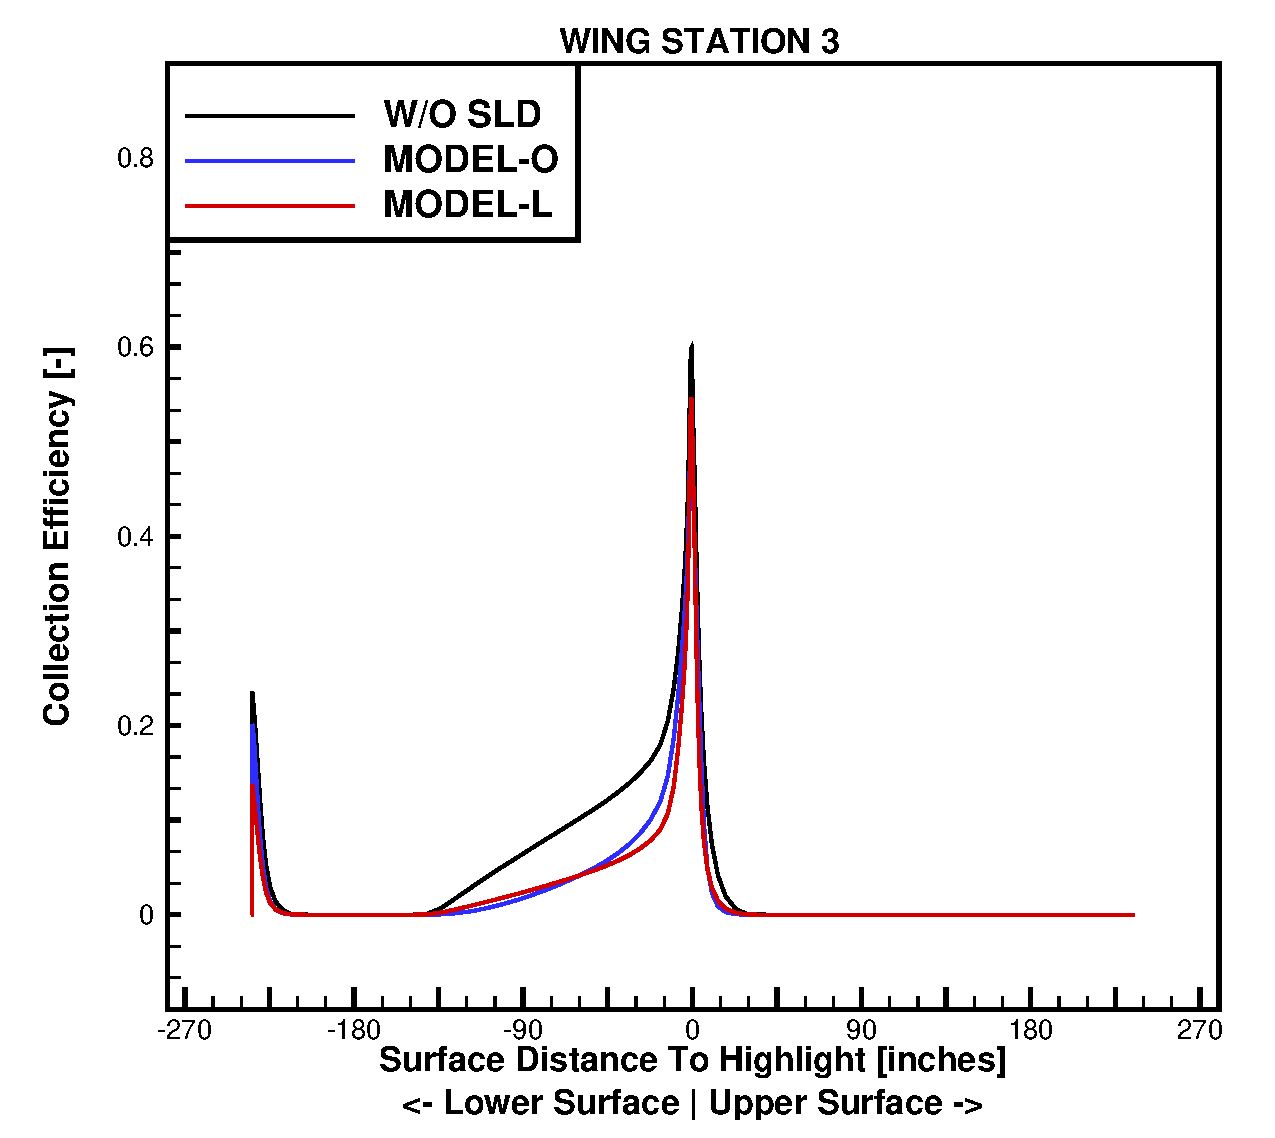
\includegraphics[width=0.325\textwidth]{FIGURES/LAGRANGIAN_ARTICLE/CASE_2p1_WING_3_SLD.eps} \quad
\label{fig:CRM_WING_3_SLD}%
}%
\subfloat[\centering SLD results on the Wing-4.]{%
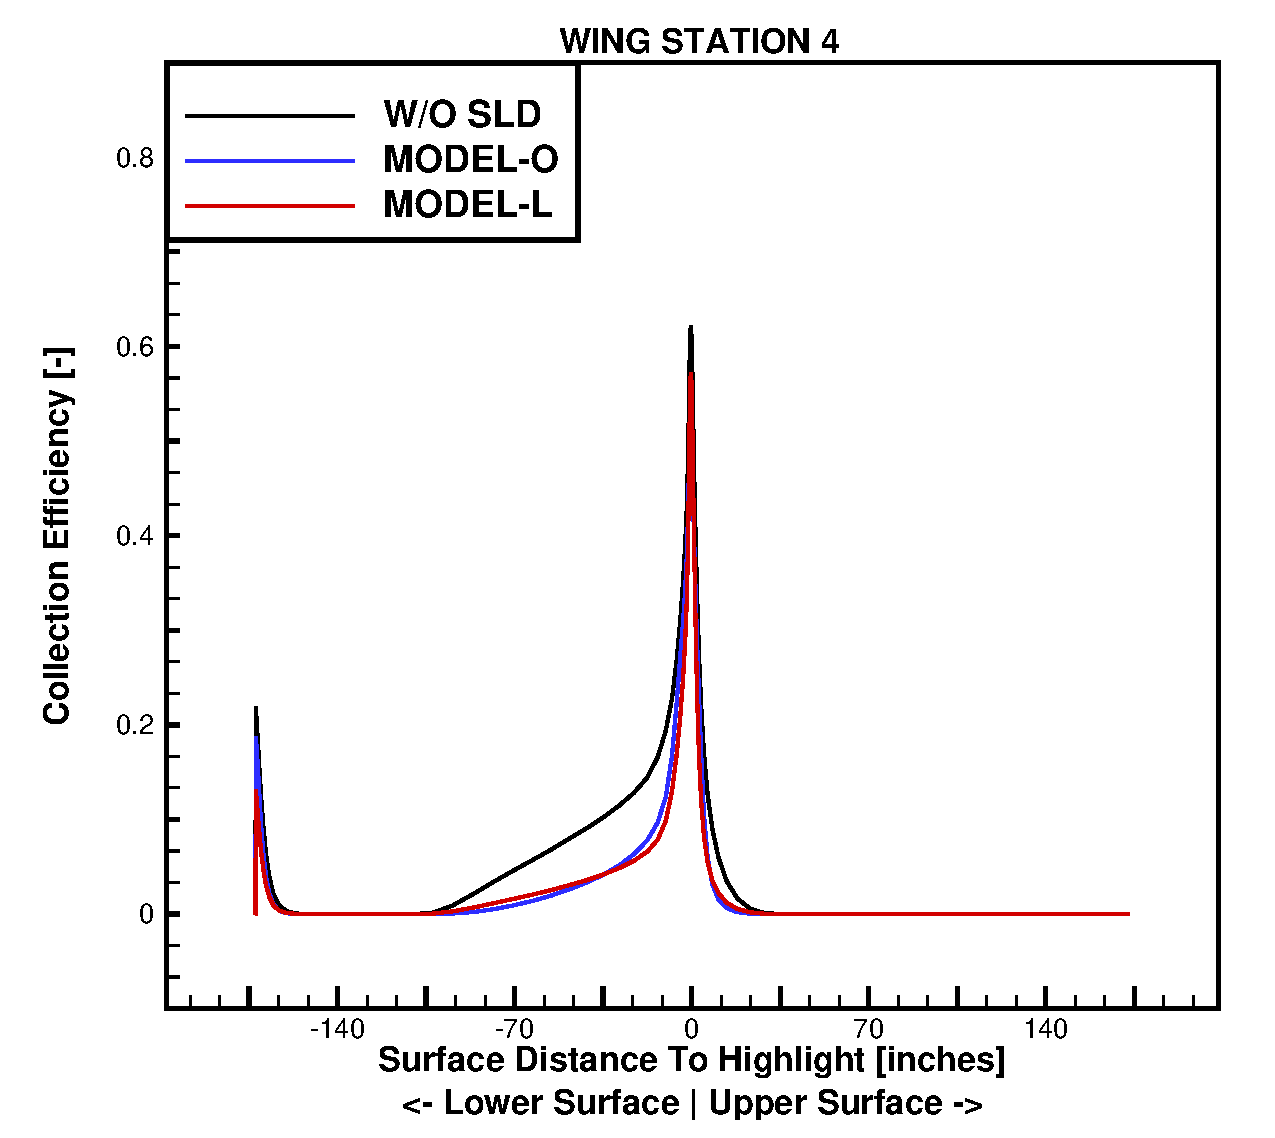
\includegraphics[width=0.325\textwidth]{FIGURES/LAGRANGIAN_ARTICLE/CASE_2p1_WING_4_SLD.eps}
\label{fig:CRM_WING_4_SLD}%
}
\subfloat[\centering SLD results on the Wing-5.]{%
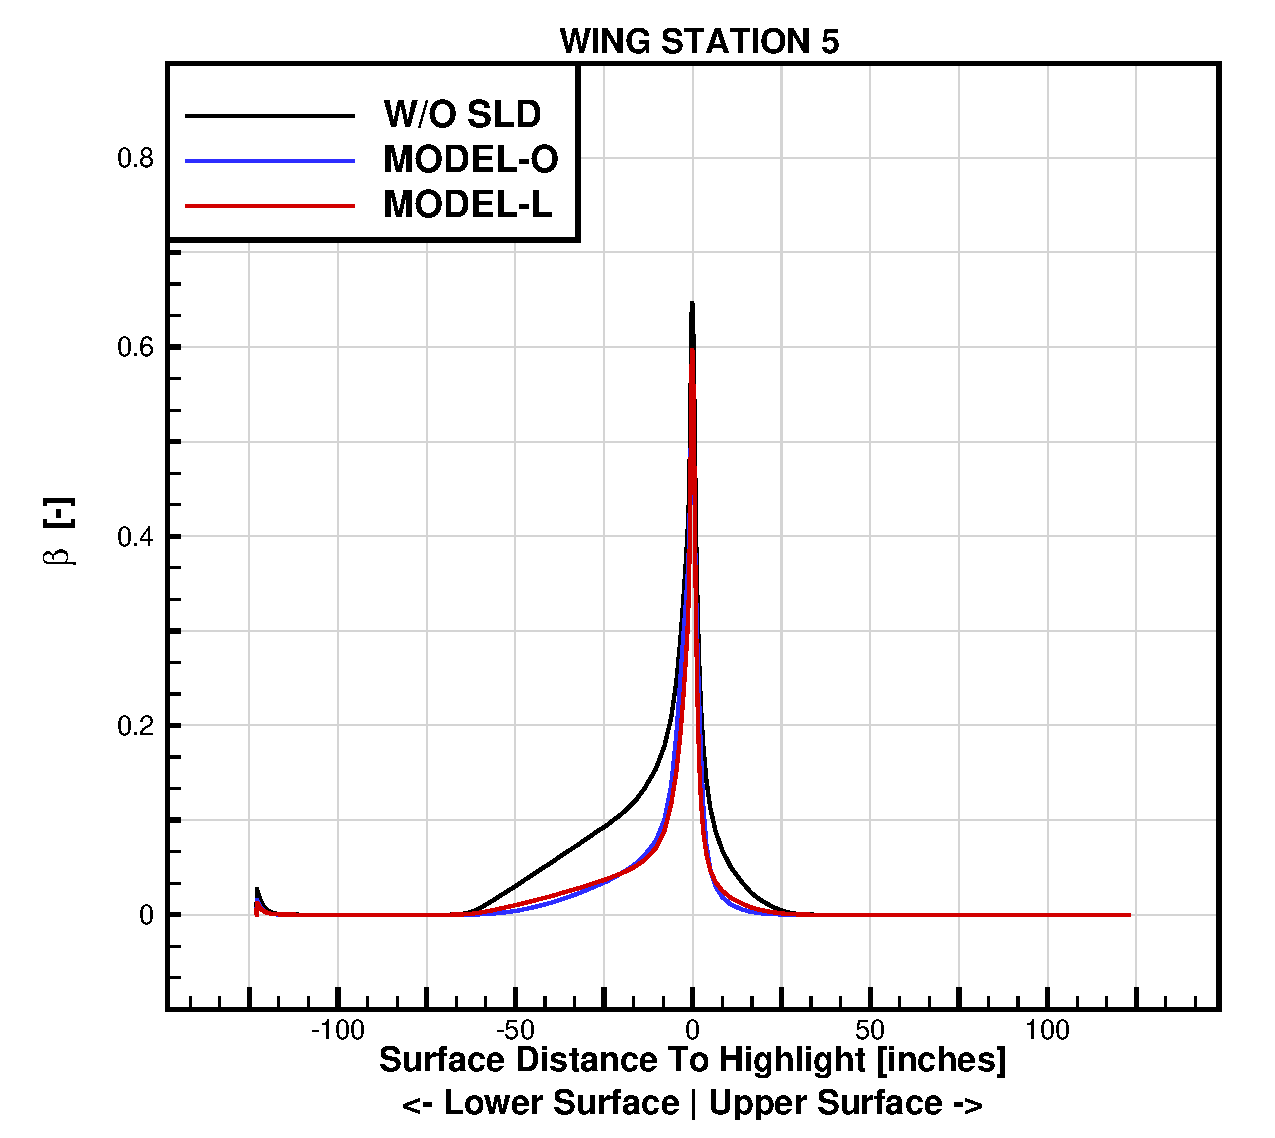
\includegraphics[width=0.325\textwidth]{FIGURES/LAGRANGIAN_ARTICLE/CASE_2p1_WING_5_SLD.eps}
\label{fig:CRM_WING_5_SLD}%
}
\caption{\centering Results for CASE HLPW5 - 2.1.}
\label{fig:2p1}
\end{figure}

For the fuselage, as shown in Fig. \ref{fig:CRM_FUSELAGE}, the peak collection efficiency is observed at the nose, gradually decreasing along the surface. The collection efficiency distribution on the wing, depicted in Fig. \ref{fig:CRM_WING_1} - \ref{fig:CRM_WING_5} exhibits a non-symmetrical shape due to the 6\textdegree $\,$ angle of attack imposed by the simulation conditions. Higher values of $\beta$ can be observed at the junction between the fuselage and the wing indicating higher impingement rate in that region. As in previous cases, more droplets are collected on the pressure side of the wing. However, since the CRM model features a swept wing, the effective angle of attack varies along the wing span. This variation is evident when comparing $\beta$ results on different hingewise cuts along the wing span. Unlike the inboard section (Fig. \ref{fig:CRM_WING_1}), the third cut shows more droplets collected on the suction side of the wing. The Lagrangian results match with the Eulerian results across all the cuts, ensuring consistency and accuracy in the simulation for such a large scale geometry.

\begin{figure}[htp] 
    \centering
    \subfloat[Collection Efficiency cuts along the wing span.]{%
        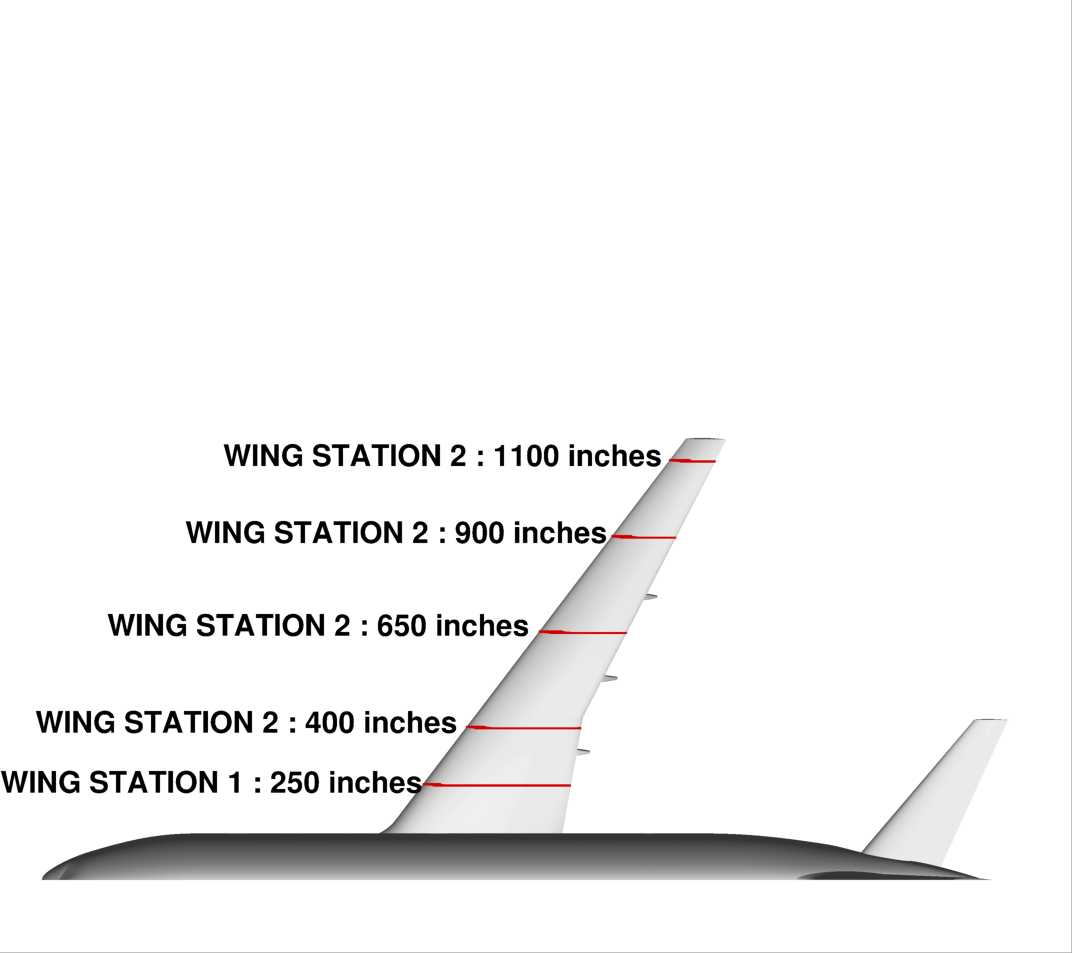
\includegraphics[trim={0.1cm 0.1cm 0.1cm 0.1cm},clip,width=0.5\textwidth]{FIGURES/LAGRANGIAN_ARTICLE/CUTS_WING.png}%
        \label{fig:wingCuts}%
        }%
    \subfloat[Collection Efficiency cut on the fuselage.]{%
        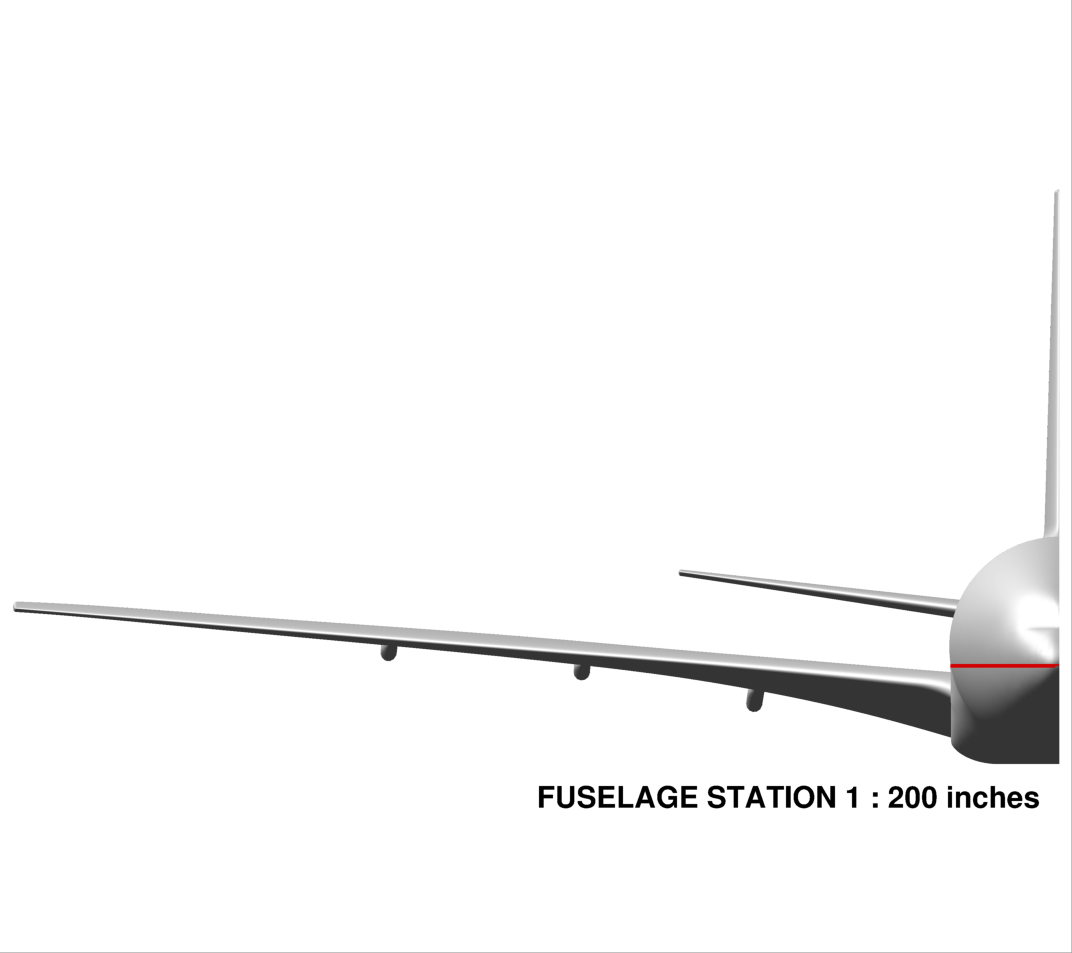
\includegraphics[trim={0.1cm 0.1cm 0.2cm 0.1cm},clip, width=0.5\textwidth]{FIGURES/LAGRANGIAN_ARTICLE/CUTS_FUSELAGE.png}%
        \label{fig:fuselageCuts}%
        }%
    \caption{Collection Efficiency cuts.}
    \label{fig:cuts}
\end{figure}

The SLD models implemented in this study exhibit consistent behavior across the full-scale CRM wing-body configuration presented in Fig. \ref{fig:CRM_FUSELAGE_SLD} - \ref{fig:CRM_WING_5_SLD}. Significant mass loss due to splashing is observed across all the cuts. Although acquiring experimental data for such a configuration is challenging, the current results align well with previous findings, demonstrating the robustness of the computational models. This consistent performance across different scales and configurations underscores the models applicability to real-world aviation scenarios.

\section{Conclusion}
\label{sec:Conclusion}

This work presents a computationally efficient framework for Lagrangian particle tracking, featuring enhancements that increase the robustness, accuracy, and overall efficiency of the solver. The trajectory-tracking algorithm that leverages mesh connectivity precisely determines droplet velocities and positions. It employs a face-to-face approach that dynamically adjusts the droplet time step based on cell size to reduce numerical instabilities, particularly in regions of strong velocity and pressure gradients near walls. A ray-tracing enhanced intersection technique is incorporated to improve the performance of intersection detection and the solver overall scalability. An adaptive seeding strategy is implemented, utilizing Eulerian droplet data to trace trajectories back to a predefined seeding plane, thereby reducing the number of tracked droplets while maintaining accuracy; this is complemented by adaptive mesh refinement of the seeding grid, driven by the accumulated collection efficiency ($\beta$) on the surface. To enhance the accuracy of $\beta$ evaluation, a weighted interpolation based on the squared inverse distance between droplet impact locations and neighboring face centers is adopted, improving droplet coverage and reducing the need for large number of droplets. The solver also incorporates Supercooled Large Droplet (SLD) physics, accounting for mass loss mechanisms such as bouncing, splashing, and rebounding upon impact, which yields a more realistic collection efficiency and closer agreement with experimental data. Finally, a hybrid Eulerian–Lagrangian strategy is discussed, in which Eulerian simulations are used to model the initial deposition while secondary droplets are tracked with the Lagrangian solver, thereby enabling efficient and accurate treatment of SLD effects and complex droplet behavior.

Benchmark cases were selected from the first and second AIAA Ice Prediction Workshops, with a large-scale configuration drawn from the fifth High-Lift Prediction Workshop. The solver achieves $94\%$ parallel efficiency on 16 nodes. Results show strong agreement between the CHAMPS Eulerian solver and the newly developed Lagrangian solver, with SLD simulations aligning more closely with experimental data than other codes reported in the literature. The hybrid Eulerian (for deposition)–Lagrangian(for secondary droplets) approach offers improvements over purely Eulerian predictions, including a slight increase in peak collection efficiency,  by combining the computational efficiency of the Eulerian solver for initial deposition with the enhanced droplet physics of the Lagrangian solver for secondary droplets, providing a promising pathway for future developments.


% \section*{Acknowledgments}
% This work is supported in part by a Bombardier/NSERC/CRIAQ Industrial Chair (first author) and a Canada Research Chair (second author). Calculations were performed on Digital Research Alliance of Canada and Calcul Quebec clusters.

% \newpage

% \section{Appendix}
% \label{sec:appendix}
% \subsection{Mesh Refinement Study}
% \label{sec:VERIF_NACA}
% \begin{table}[h!]
% \centering
% \caption{Simulation Parameters}
% \begin{tabular}{cccccc}
% \hline \hline
% Description & MVD[$\mu m$] & AOA[\textdegree]& Ma[-]& C$_{ref}$[inch] & Re[-]\\
% \hline
% NACA0012 & 30.0 & 5.0 & 0.4 & 1.0 & 8.85 $\cdot 10^6$ \\
% \hline \hline
% \end{tabular}
% \label{tab:naca0012_VERIF}
% \end{table}

% \begin{figure}[h!]
% \centering
% \subfloat[\centering Impingement Results on the 129x129 mesh.]{%
% 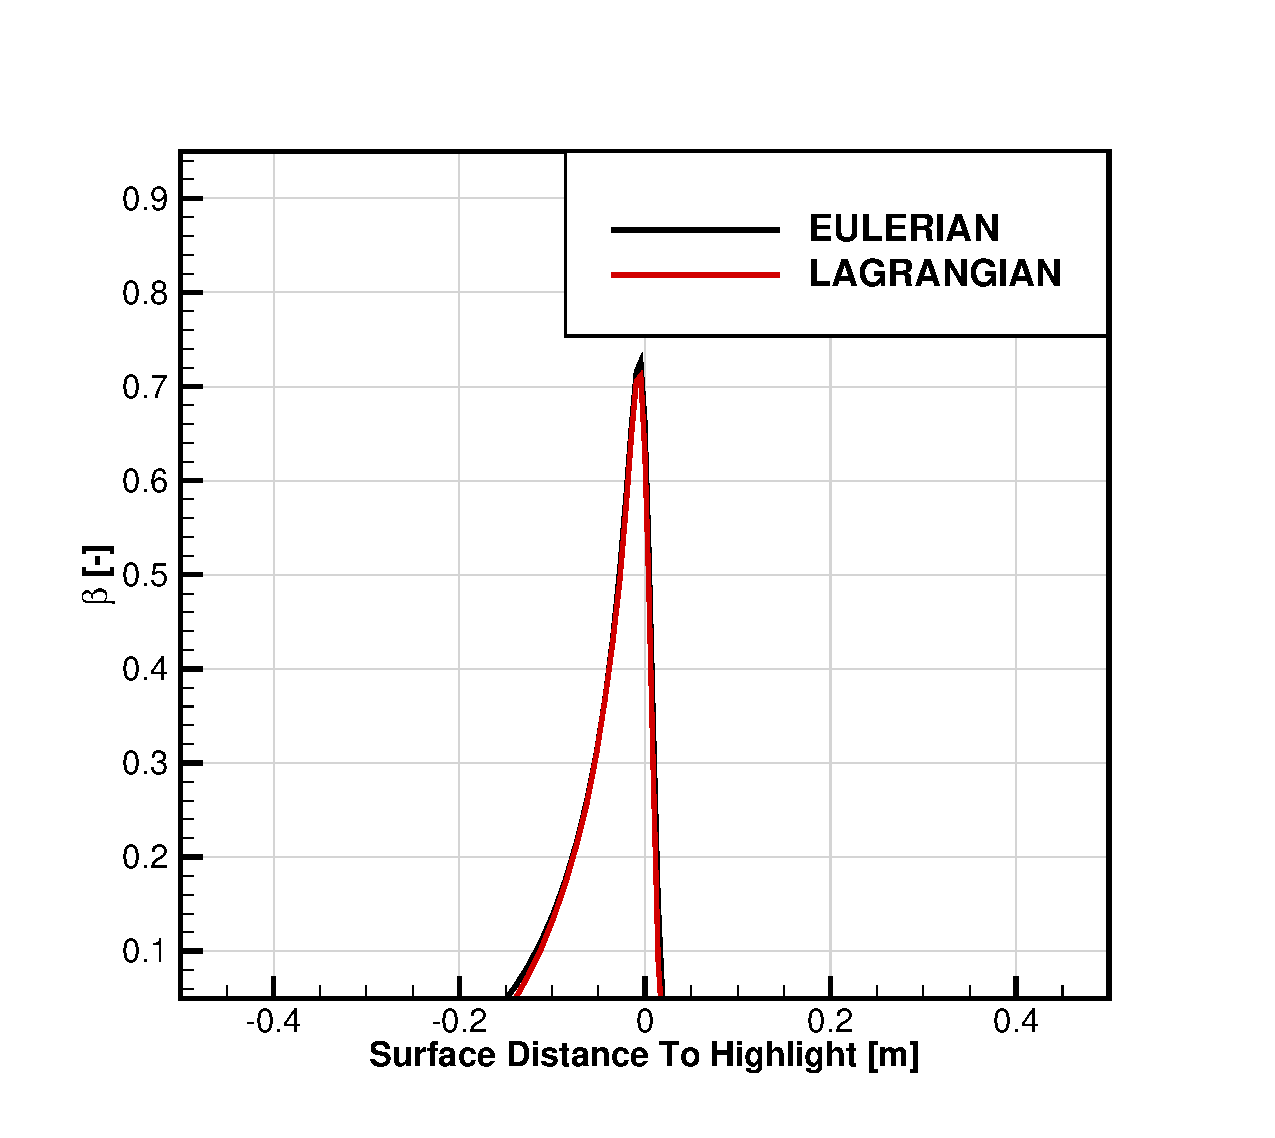
\includegraphics[trim={0cm 0.05cm 0.05cm 0cm}, clip, width=0.4\textwidth]{FIGURES/LAGRANGIAN_ARTICLE/NACA0012_129.eps}
% \label{fig:NACA0012_129}%
% }
% \subfloat[\centering Impingement Results on the 257x257 mesh.]{%
% 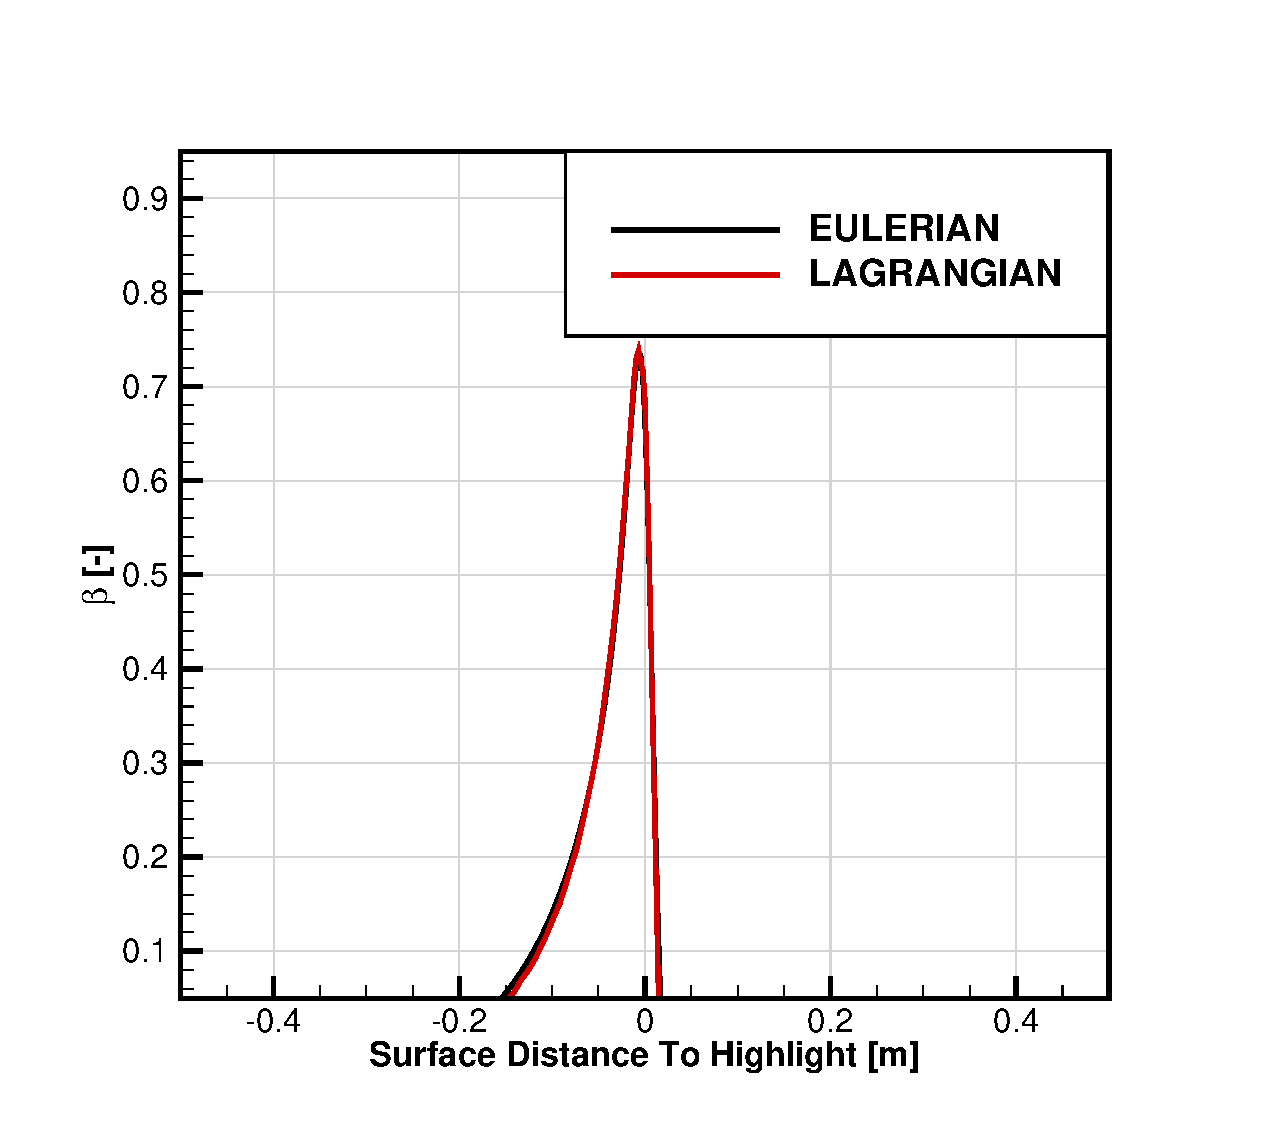
\includegraphics[trim={0cm 0.05cm 0.05cm 0cm}, clip, width=0.4\textwidth]{FIGURES/LAGRANGIAN_ARTICLE/NACA0012_257.eps}
% \label{fig:NACA0012_257}%
% }

% \hspace*{-1cm}

% \centering
% \subfloat[\centering Impingement Results on the 513x513 mesh.]{%
% 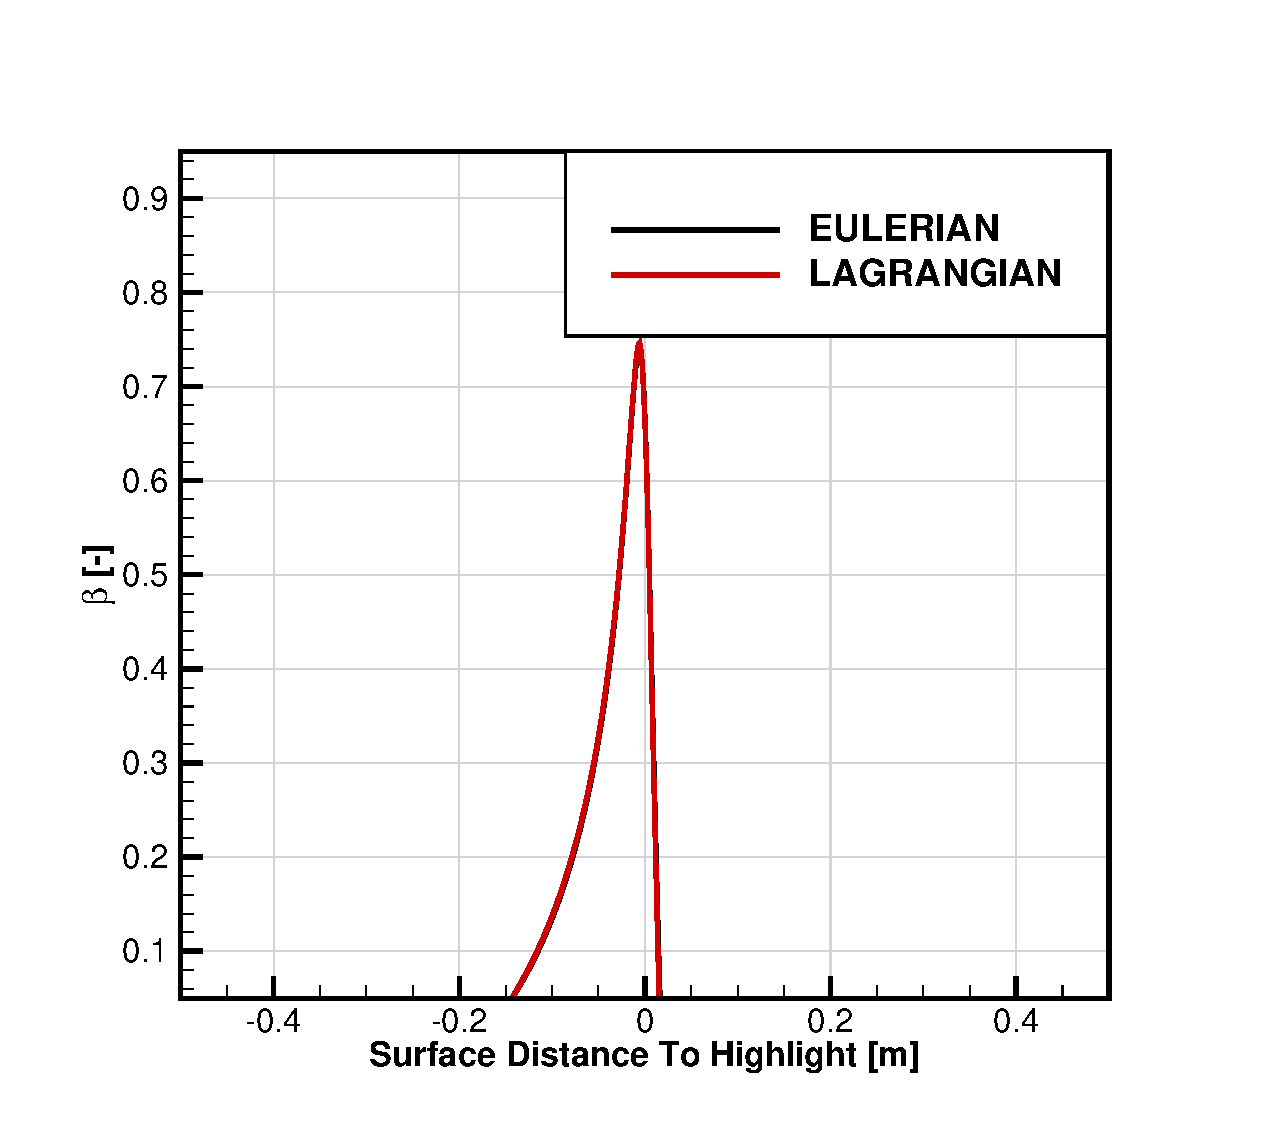
\includegraphics[trim={0cm 0.05cm 0.05cm 0cm}, clip, width=0.4\textwidth]{FIGURES/LAGRANGIAN_ARTICLE/NACA0012_513.eps}
% \label{fig:NACA0012_513}%
% }%
% \subfloat[\centering Impingement Results on the 1025x1025 mesh.]{%
% 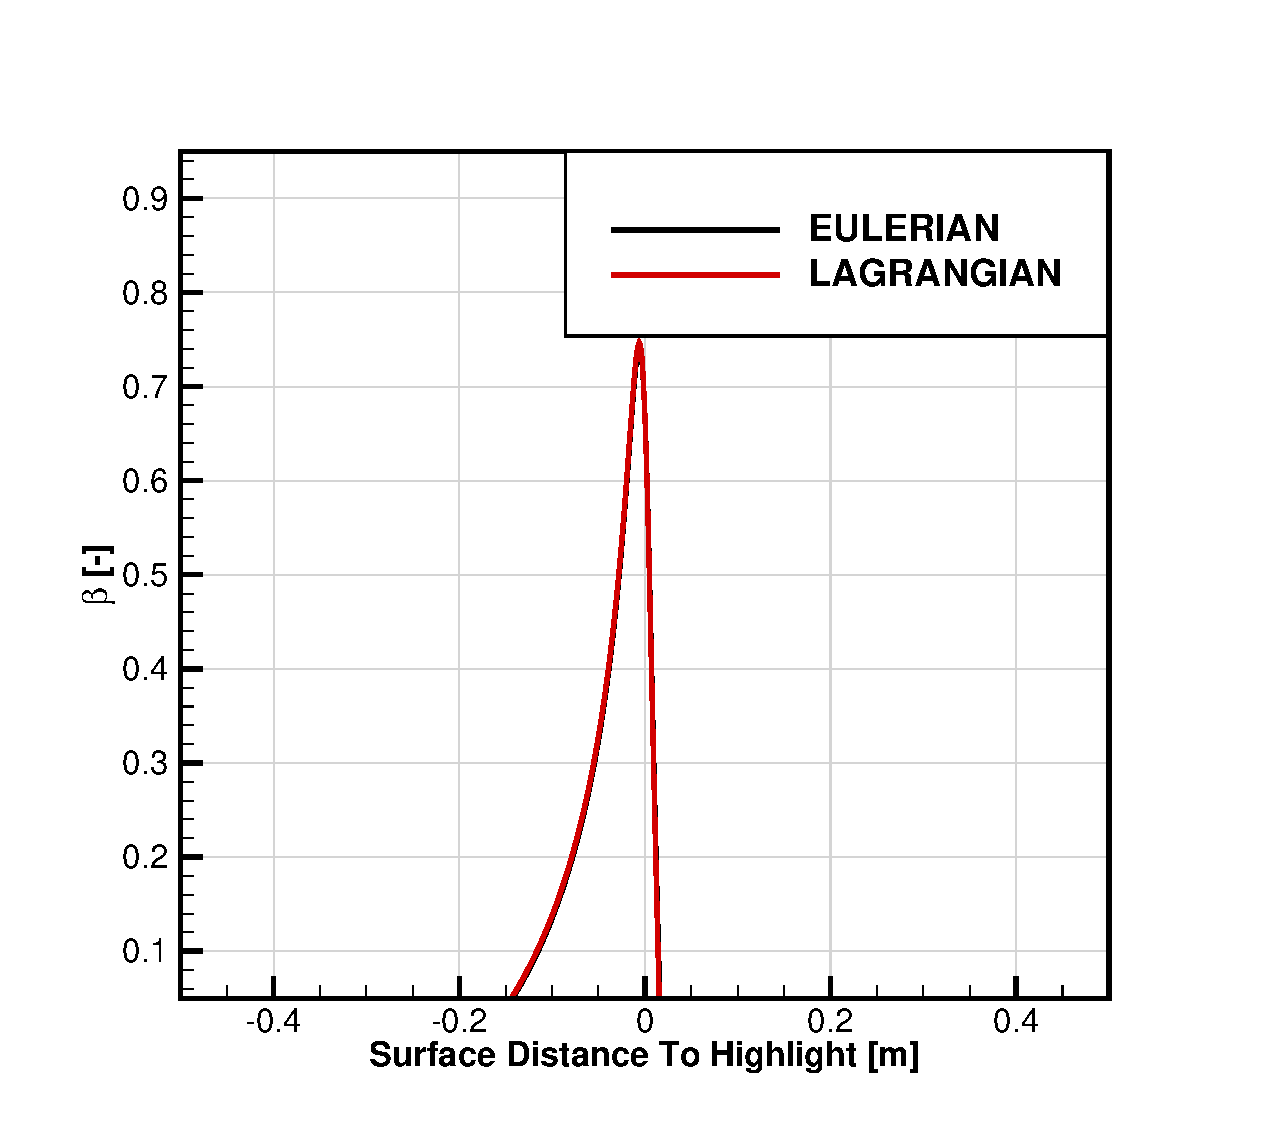
\includegraphics[trim={0cm 0.05cm 0.05cm 0cm}, clip, width=0.4\textwidth]{FIGURES/LAGRANGIAN_ARTICLE/NACA0012_1025.eps}   
% \label{fig:NACA0012_1025}}
% \caption{Mesh refinement effect on the Eulerian vs. Lagrangian results in terms of the collection efficiency.}
% \label{fig:NACA0012_VERIF}
% \end{figure}


% \begin{table}[h!]
% \centering
% \caption{Difference Between Eulerian vs. Lagrangian results in terms of Collection Efficiency.}
% \begin{tabular}{cc}
% \hline \hline
% Mesh & Max Difference $\beta$ [-]\\
% \hline
% 129x129 & $0.069$ \\ \hline
% 257x257 & $0.059$ \\ \hline
% 513x513 & $0.037$ \\ \hline
% 1025x1025 & $0.035$ \\ \hline
% \hline
% \end{tabular}
% \label{tab:naca0012_VERIF_error}
% \end{table}

% \newpage

% \subsection{SLD Models details}
% \label{app:sldModels}
% Table~\ref{tab:splashing_Models_dets} provides the parameters used for the SLD models described in Section~\ref{Sec:SLDEffects}.

% \begin{table}[h!]
% \centering
% \caption{SLD Splashing Models Details}
% \label{tab:splashing_Models_dets}
% \begin{tabular}{ccc}
% \hline \hline
% \multicolumn{3}{c}{Wright et al. \cite{wright2004semi}}\\ 
% \hline
%  $\theta_0$ & Droplet Angle of Impact & -\\
%  $K_{M}$ & Splashing Parameter & $ \frac{0.859 \,  K^{0.5} \, (\frac{\rho_{w}}{LWC})^{0.125}}{sin(\theta_0)^{1.25}} $ \\
%   $K$ & Mundo Parameter & $Oh \, Re_d^{1.25}$ \\
%   $Oh$ & Ohnesorge Number & $\frac{\mu_w}{\sqrt{\sigma_w \, \rho_w \, D}}$ \\
%  \hline
%  \multicolumn{3}{c}{Trontin et al. \cite{trontin2016revisited}}\\ 
%  \hline
%   $\theta_c$ & Characteristic Droplet Angle of Impact & $25.0$\textdegree \\
%   $\theta_c$ & Critical Droplet Angle of Impact &  $\theta_0 \, tanh(Ca^{1.5})$ \\
%   $Ca$ & Capillary Number & $\frac{\mu_{w} \vert \boldsymbol{u_d} \vert}{\sigma_{w}}$ \\
%   $K_C$ & Cossali Number & $We \, Oh^{-0.4}$ \\
%   $We $ & Weber Number & $ \frac{\rho_{w} \vert \boldsymbol{u_d} \vert ^2  d}{\sigma_{w}}$ \\
%   $K_0$ & Critical Cossali Number & $657.0$ \\
%   $g(\frac{\theta}{\theta_c})$ & Angle of Impact Function & $1 \, if \, \theta \, > \, \theta_c \, else \, \frac{\theta}{\theta_c}$ \\
%   $f(\Tilde{K_c})$ & Cossali Number Function & $1 - 0.15 \frac{\Tilde{K_c}^2}{(100+\Tilde{K_c}^2)}$ \\
%   $\Tilde{K_c}$ & - & $max (\frac{K_c - K_0}{K_0},0)$\\
% \hline \hline
% \end{tabular}
% \end{table}

% \newpage

% \subsection{Test-Case Geometries}
% \label{app:geometries}
%   \begin{figure}[htbp] 
%     \centering
%     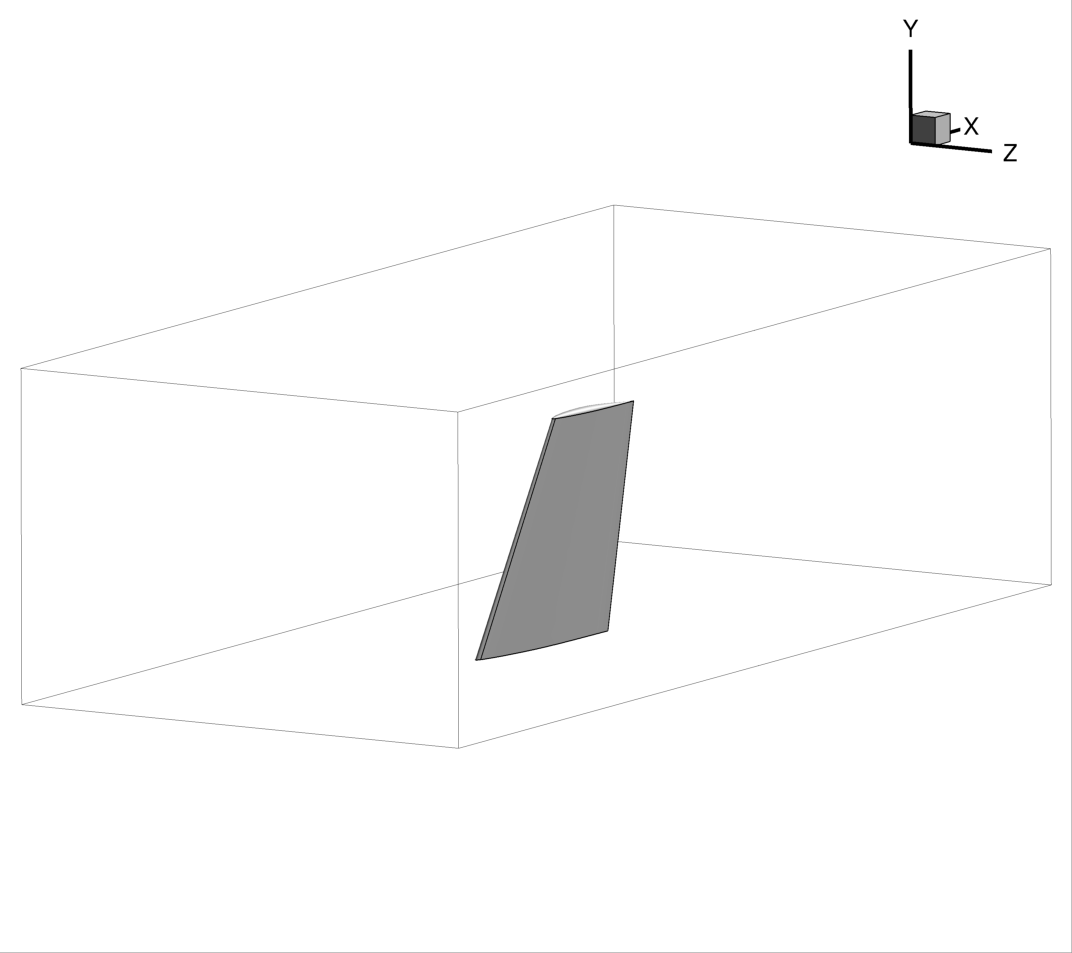
\includegraphics[trim={0cm 0cm 0cm 0cm},clip,width=0.7\textwidth]{FIGURES/LAGRANGIAN_ARTICLE/HTAIL.png}
%     \caption{Description of Case IPW1 - 112.}
%     \label{fig:htailGeo}
% \end{figure}



